\documentclass[12pt, oneside, a4paper, final]{memoir}
%TC:group tabular 1 1
%TC:group table 0 1
%TC:macro \footnote [text]
%TC:ignore
\setlrmarginsandblock{2cm}{2cm}{*}
\setulmarginsandblock{2cm}{2cm}{*}
\checkandfixthelayout
\title{Title Here}
\newcommand{\thesubtitle}{Subtitle Here}
\author{Author Here}
\date{\today}
\newcommand{\tripos}{Tripos \& Part Here}
\newcommand{\degree}{Bachelor of Arts}
\newcommand{\university}{University of Cambridge}
\newcommand{\college}{College Here}
\newcommand{\supervisors}{Supervisor 1, Supervisor 2}
\newcommand{\candidatenumber}{Candidate Number Here}
\newcommand{\submissiondeadline}{MM/YYYY Submission Month Deadline Here}
\newcommand{\projectoriginator}{Project Originator Here}
\usepackage{graphicx}
\usepackage[utf8]{inputenc}
\usepackage[backend=biber, style=ieee]{biblatex}
\usepackage{amsmath}
\usepackage{amssymb}
\usepackage{stmaryrd}

\usepackage{semantic}

\usepackage{minted}
\usemintedstyle{colorful}

\usepackage[font=small,labelfont=bf]{caption}

\usepackage[dvipsnames]{xcolor}
\usepackage[normalem]{ulem}
\makeatletter
\def\uwave{\bgroup \markoverwith{\lower3.5\p@\hbox{\sixly \textcolor{red}{\char58}}}\ULon}
\font\sixly=lasy6 % does not re-load if already loaded, so no memory problem.
\makeatother

\usepackage{soul}


\newcommand{\hlc}[2][yellow]{{%
    \colorlet{foo}{#1}%
    \sethlcolor{foo}\hl{#2}}%
}
\newcommand{\error}[1]{\hlc[pink!50]{#1}}
\newcommand{\hlcmaths}[2][yellow!50]{\colorbox{#1}{$\displaystyle #2$}}

\newcommand{\code}[1]{\text{\mintinline[escapeinside=||]{reason}{#1}}}
\newcommand{\casthl}[4][yellow!50]{\ensuremath{\code{#4}^{\text{\hlc[#1]{${\langle$\code{#2}$ \Rightarrow $\code{#3}$\rangle}$}}}}}
\newcommand{\cast}[3]{\casthl[red!0]{#1}{#2}{#3}}
\newcommand{\casterror}[3]{\casthl[pink!50]{#1}{#2}{#3}}

\newcommand{\hole}[1][]{{\color{red}\llparenthesis} #1 {\color{red}\rrparenthesis}}
\newcommand{\scast}[2]{{\color{blue}\langle} #1 {\color{blue}\Rightarrow} #2 {\color{blue}\rangle}}
\newcommand{\scastfail}[2]{{\color{blue}\langle} #1 {\color{blue}\Rightarrow} ? {\color{blue}\nRightarrow} #2 {\color{blue}\rangle}}
\newcommand{\synthesis}[3][\Gamma]{#1 \vdash #2 {\color{BrickRed}\ \Rightarrow}\ #3}
\newcommand{\analysis}[3][\Gamma]{#1 \vdash #2 {\color{BlueViolet}\ \Leftarrow}\ #3}
\newcommand{\typeassignment}[3][\Delta;\Gamma]{#1 \vdash #2 : #3}
\newcommand{\elaborationSynthesis}[5][\Gamma]{#1 \vdash #2 {\color{BrickRed}\ \Rightarrow\ } #3 \leadsto #4 \dashv #5}
\newcommand{\elaborationAnalysis}[6][\Gamma]{#1 \vdash #2 {\color{BlueViolet}\ \Leftarrow\ } #3 \leadsto #4 : #5 \dashv #6}

\newcommand{\funmatch}{\blacktriangleright_\rightarrow}

\addbibresource{References/refs.bib}
\makeindex


\usepackage{hyperref}
\hypersetup{
    colorlinks=true,
    linkcolor=blue,
    filecolor=magenta,      
    urlcolor=cyan,
    pdftitle={\theauthor: \thetitle},
    pdfpagemode=FullScreen,
    }

\urlstyle{same}

%TC:group tabular 1 1
%TC:group table 0 1
%TC:macro \footnote [text]

\newcommand{\wordcount}{\input{|"texcount -inc -sum -0 \jobname.tex"}}

\setsecnumdepth{subsection}
\usepackage{etoolbox}
\setlrmarginsandblock{2cm}{2cm}{*}
\setulmarginsandblock{2cm}{4cm}{*}
\checkandfixthelayout 

\usepackage{letltxmacro}

\LetLtxMacro\Oldfootnote\footnote

\newcommand{\EnableFootNotes}{%
  \LetLtxMacro\footnote\Oldfootnote%
}

\newcommand{\DisableFootNotes}{%
  \renewcommand{\footnote}[2][]{\relax}
}



\makepagestyle{myruled}
\makeheadrule{myruled}{\textwidth}{\normalrulethickness}
\makeevenhead{myruled}{\bfseries\rightmark}{}{\hspace{1cm}\bfseries\thepage}
\makeoddhead{myruled}{\bfseries\rightmark}{}{\hspace{1cm}\bfseries\thepage}
\makefootrule{myruled}{\textwidth}{0pt}{0pt} % suppress bottom rule
\makeevenfoot{myruled}{}{}{}
\makeoddfoot{myruled}{}{}{}

% Ensure section titles are marked for headers
\makeatletter
\renewcommand{\sectionmark}[1]{\markright{\thesection\quad #1}}
\makeatother
\makeatletter
\renewcommand{\chaptermark}[1]{\markright{\thechapter\quad #1}}
\makeatother


\makechapterstyle{custom}{%
  \chapterstyle{default}
  \renewcommand*{\chapnamefont}{%
    \normalfont\normalsize\raggedright}
  \renewcommand*{\chaptitlefont}{%
    \normalfont\Large\bfseries\raggedright}
  \renewcommand*{\chapternamenum}{}
  \setlength{\chapindent}{0in}
  \setlength\midchapskip{0.5ex}\renewcommand*{\afterchapternum}{}
  \renewcommand*{\printchapternum}{\space\chapnamefont\bfseries\thechapter}
	\setlength{\beforechapskip}{-2\baselineskip}       	\setlength{\afterchapskip}{1.5ex}
  \renewcommand*{\printchaptertitle}[1]{
      \hrulefill\ \thepage\vskip\midchapskip
      \raggedleft \chaptitlefont ##1\par\nobreak}
}

\aliaspagestyle{chapter}{empty}
\begin{document}

\frontmatter

\begin{titlingpage}
\begin{flushright}

        \textbf{\theauthor}
\end{flushright}
\begin{center}


        \vspace*{1cm}
            
        \Huge
        \textbf{\thetitle}
            
        \vspace{0.5cm}
        \LARGE
        \tripos
            
        \vspace{1.5cm}
            
            

        
\includegraphics[width=0.4\textwidth]{Media/Crests/Sidney_Sussex}            
            
        \Large
        \college\ College\\
        \university
        
        \thedate
        \vfill
        
        \normalsize
        \textit{A dissertation submitted to the \university\ in partial fulfilment for a \degree}
            
    \end{center}
\end{titlingpage}
\setlength{\beforechapskip}{10pt}
\pdfbookmark[1]{Declaration}{Declaration of Originality}
\section*{Declaration of Originality}
I, the candidate for Part II of the Computer Science Tripos with Blind Grading Number 2328E, hereby declare that this report and the work described in it are my own work, unaided except as may be specified below, and that the report does not contain material that has already been used to any substantial extent for a comparable purpose. In preparation of this report, I adhered to the Department of Computer Science and Technology AI Policy. I am content for my report to be made available to the students and staff of the University. 
Date 12/05/2025
\pdfbookmark[1]{Proforma}{Proforma}
\chapter*{Proforma}
\begin{tabularx}{\linewidth}{l X}
Candidate Number: & \textbf{\candidatenumber}\\
College: & \textbf{\college}\\
Project Title: & \textbf{\thetitle}\\
Examination: & \textbf{\tripos\ -- \submissiondeadline}\\
Word Count: & \textbf{\wordcount}\footnote{\textit{Calculated by \texttt{texcount}. Including: tables and footnotes. Excluding: the front matter,  bibliography, and appendices}}\\
Code Line Count: & \textbf{Code Count} \footnote{\textit{Calculation method here}}\\
Project Originator: & \textbf{\projectoriginator}\\
Supervisors: & \textbf{\supervisors}
\end{tabularx}

\section*{Original Aims of the Project}
Aims Here. Concise summary of proposal description.

\section*{Work Completed}
Work completed by deadline.

\section*{Special Difficulties}
Any Special Difficulties encountered

\chapterstyle{custom}


\titlespacing*{\section}{0pt}{1.5ex plus .2ex minus .1ex}{1ex}
\titlespacing*{\subsection}{0pt}{1.5ex plus .2ex minus .1ex}{1ex}
\titlespacing*{\subsubsection}{0pt}{1.5ex plus .2ex minus .1ex}{0.5ex}
\titlespacing*{\paragraph}{0pt}{1ex}{1em}

% Section
\titleformat{\section}
  {\normalfont\large\bfseries}
  {{\thesection}.}
  {1em}
  {#1}

% Subsection
\titleformat{\subsection}
  {\normalfont\normalsize\bfseries}
  {\thesubsection.}
  {1em}
  {#1}

% Subsubsection
\titleformat{\subsubsection}
  {\normalfont\normalsize\bfseries}
  {}
  {0pt}
  {#1}

% Paragraph
\titleformat{\paragraph}[runin]
  {\normalfont\bfseries}
  {}
  {0pt}
  {#1}
  [:]

\newpage

\pagestyle{myruled}
\setlrmarginsandblock{2cm}{2cm}{*}
\setulmarginsandblock{2cm}{1.2cm}{*}
\setheaderspaces{*}{4pt}{*}
\checkandfixthelayout[fixed]
%\DisableFootNotes

\setcounter{tocdepth}{2}
\pdfbookmark[1]{Contents}{Contents}
\tableofcontents*

%\DisableFootNotes
%TC:endignore
\setSpacing{0.948}
\mainmatter

\chapter{Introduction}
\label{chap:Introduction}
Software bugs are an inherent part of programming, often leading to unexpected behaviour and system failures. Debugging these errors is a \textit{time-consuming process} taking between 20-60\% of active work time \cite{DebugTimeSelfReport}, with programmers spending a \textit{highly skewed} proportion of their time identifying and resolving a small proportion of \textit{difficult} bugs \cite{DebugSkew}.

Type systems aim to alleviate some of this burden by classifying expressions and operations that are allowed to work on them. This may be done \textit{statically} at compile time or \textit{dynamically} during runtime. The expressions not conforming to the type system manifest themselves as \textit{type errors}.

In static typing, blame for type errors are typically localised to a \textit{single} location in the code. However, this localisation may be misleading, as the actual cause of the error might be rooted in a broader context, for example in OCaml 65\% of type errors related to \textit{multiple} locations \cite{StudentTypeErrorFixes}. This is a particularly prevalent issue in \textit{type inferred} languages.

In dynamic typing, type errors are often missed as they only appear during runtime with specific inputs.
Additionally, they don't generally specify any source code context which caused them. Instead, a dynamic type error is accompanied by an \textit{evaluation trace}, which can be \textit{more intuitive} \cite{TraceVisualisation} by demonstrating concretely why values are \textit{not} consistent with their expected type as required by a \textit{runtime cast}.

This project seeks to improve user understanding of type errors by localising static type errors \textit{more completely}, and \textit{combining} the benefits of static and dynamic type errors.

I consider three research problems and implement three features to solve them in the Hazel language \cite{Hazel}:\footnote{The answers may differ greatly for other languages. Hazel provides a good balance between complexity and usefulness.}
\begin{enumerate}
\item Can we statically highlight code which explains \textit{static type errors} more \textit{completely}, including all code that \textit{contributes} to the error? 

This would alleviate the issue of static errors being \textit{incorrectly localised}, and help give a \textit{greater context} to static type errors.

\textbf{Solution:} I devise a \textit{novel} method of \textbf{type slicing} including formal mathematical foundations built upon the formal \textit{Hazel calculus} \cite{HazelLivePaper}. Additionally, it generalises to highlight all code relevant to typing \textit{any} expressions (not just erroneous expressions).

\item Can we dynamically highlight source code which contributes to a \textit{dynamic type error}?

This would provide missing source code context to understand how types involved in a dynamic type error originate from the source code.

\textbf{Solution:} I devise a \textit{novel} method of \textbf{cast slicing}, also with formal mathematical foundations. Additionally, it generalises to highlight source code relevant to requiring any specific \textit{runtime casts}.

\item Can we provide dynamic \textit{evaluation traces} to explain \textit{static type errors}?

This would provide an \textit{intuitive} concrete explanation for static type errors.

\textbf{Solution:} I implement a \textbf{type error witness search procedure}, which discovers inputs (witnesses) to expressions which cause a \textit{dynamic type error}. This is based on research by Seidel et al. \cite{SearchProc} which devised a similar procedure for a subset of OCaml.
\end{enumerate}

Hazel \cite{Hazel} is a functional locally inferred and gradually typed research language allowing the writing of \textit{incomplete programs} under active development at the University of Michigan. Being gradually typed, allowing both static and dynamic code to coexist, this project successfully demonstrates the utility of these three features in improving understanding of \textit{both} static and dynamic errors. Both, to a \textit{greater extent} than in any existing languages, with the explanations being \textit{useful} in debugging type errors, and is expected to reduce debugging times and aid in students understanding type systems.\footnote{Proving this would require a user study.}

\prargraph{Example:} \textit{A basic well-formatted \textbf{graphical} walk-through for how a static type error could be diagnosed using the three features. Take simplest example from the evaluation.}

\begin{figure}

\caption{A Static Type Error}
\label{fig:ErrorExample}
\end{figure}

\section{Related Work}
\label{sec:RelatedWork}
There has been extensive research into attempting to understand \textit{what} is needed \cite{DebugNeeds}, \textit{how} developers fix bugs \cite{HowFixBugs}, and a plethora of compiler \textit{improvements} and \textit{tools} \textbf{add citations here, primarily functional language tools}. This project builds upon this body of research in new ways focusing on the Hazel language, which is itself a research project being taken in various directions (\textbf{cite the directions}) but generally as a \textit{teaching language} (\textbf{cite the explainthis paper}) for students. 

To my knowledge the ideas of \textit{type slicing} and \textit{cast slicing} are novel. However, they do output \textit{program slices} which were originally explored by Weiser \cite{ProgSlice}, though my definition of program slices matches more with functional program slices \cite{FunctionalProgExplain}.  The properties I explore are more similar to \textit{dynamic program slicing} \cite{DynProgSlice} but with type characteristics rather than evaluation characteristics, in a sense similar \textit{type error slicing} \cite{ErrSlice}.

The \textit{type witness search procedure} is	 based upon Seidel et al. \cite{SearchProc}, though there are significant differences in workings due to my use of Hazel and various extensions as compared to the subset of OCaml used by Seidel et al.

\section{Dissertation Outline}
\label{sec:Outline}
\Cref{chap:Preparation} introduces the \textit{type theories} (\cref{sec:TypeSystems}) underpinning the \textit{Hazel core calculus} (\cref{sec:CoreHazel}), followed by basic background on the \textit{Hazel implementation} (\cref{sec:HazelImplementation}). Additionally, methods of non-deterministic programming are introduced (\cref{sec:Nondeterminism}).

\Cref{sec:TypeSlicingTheory} and \cref{sec:CastSlicingTheory} formalise and prove\footnote{TODO} the ideas of \textit{type slices} and \textit{cast slices} in the Hazel core calculus. 
 
 An implementation (\cref{sec:TypeSlicingImplementation}-\ref{sec:CastSlicingImplementation}) of these has been created covering \textit{most}\footnote{Except for type substitution.} of the Hazel language, including a user interface. 
 
 A \textit{type witness search procedure} was successfully implemented. This involved creating a \textit{hole instantiation} and a simplified \textit{hole substitution} method (\cref{sec:HoleInstantiation}); there is currently no full hole substitution feature in Hazel despite it's presence in the core calculus (\cref{sec:HoleSubstitution}). Additionally, a customisable instantiation method was implemented (\cref{sec:Stepper}) controllable via a UI.\footnote{TODO}

The slicing features and search procedure met all goals, \textbf{list eval goals briefly}, showing \textit{effectiveness} (\cref{sec:EffectivenessAnalysis}) and being reasonably \textit{performant} (\cref{sec:PerformanceAnalysis}) over a corpus of \textit{well-typed} and \textit{ill-typed} Hazel programs respectively (\cref{sec:CorpusCollection}). Further, considered deviations from the slicing theories and strengths and weaknesses of the search procedure were evaluated in detail (\cref{sec:CriticalAnalysis}). A cognitive walk-through is performed in \cref{sec:CognitiveWalkthrough} considering the use of all the features in debugging the static type error presented in the introduction in \cref{fig:StaticError}.

Finally, further directions and improvements have been presented along with discussion on the applicability of these features, slicing in particular, to real world debugging situations in \cref{chap:Conclusions}.
\chapter{Preparation}
\label{chap:Preparation}
In this chapter I present the technical background knowledge for this project: an introduction to the type theory for understanding Hazel's core semantics, an overview of Hazel implementation, and notes on non-determinism (as the type witness search procedure is non-deterministic). Following this, I present my software engineering methodology.

\section{Background Knowledge}\label{sec:BackgroundKnowledge}
\subsection{Static Type Systems}\label{sec:TypeSystems}
A \textit{type system} is a lightweight formal mathematical method which categorises values into \textit{types} and expressions into types that evaluate to values of the same type. It is effectively a static \textit{approximation} to the runtime behaviour of a language. 

\subsubsection{Syntax}
Trivial, probably not needed? Cite BNF grammars etc. All Ib stuff.
Maybe briefly show examples of Lambda calculus-like syntax?
\subsubsection{Judgements \& Inference Rules}\label{sec:Judgements}
A \textit{judgement}, $J$, is an assertion about \textit{expressions} in a language \cite{PracticalFoundations}. For example: \begin{itemize}
\item $\mathrm{Exp\ e}$ -- $e$ is an \textit{expression} 
\item $n : \code{int}$ -- $n$ has type \code{int}
\item $e \Downarrow v$ -- $e$ evaluates to \textit{value} $v$ 
\end{itemize}
While an \textit{inference rule} is a collection of judgements $J, J_1, \dots, J_n$:
\[\inference{J_1 & J_2 & \dots & J_n}{J}\]
Representing the \textit{rule} that if the \textit{premises}, $J_1, \dots, J_n$ are true then the conclusion, $J$, is true. When the collection of premises is empty, it is an \textit{axiom} stating that the judgement is \textit{always} true. Truth of a judgement $J$ can be assessed by constructing a \textit{derivation}, a tree of rules where it's leaves are axioms. It is then possible to define a judgement as the largest judgement that is \textit{closed} under a collection of rules. This gives the result that a judgement $J$ is true \textit{if and only if} it has a derivation.

Properties on expressions can be proved using \textit{rule induction}, if a property is \textit{preserved} by every rule for a judgement, and true for it's axioms, then the property holds whenever the judgement is derivable.

A \textit{hypothetical judgement} is a judgement written as: 
\[J_1, \dots, J_n \vdash J\]
is true if $J$ is derivable when additionally assuming each $J_i$ are axioms. Often written $\Gamma \vdash J$ and read \textit{$J$ holds under context $\Gamma$}. Hypothetical judgements can be similarly defined inductively via \textit{rules}.

\subsubsection{Defining a Type System}\label{sec:TypingJudgements}
A typical type system can be expressed by defining the following hypothetical judgement form $\Gamma \vdash e : \tau$ read as \textit{the expression $e$ has type $\tau$ under typing context $\Gamma$} and referred as a \textit{typing judgement}. Here, $e : \tau$ means that expression $e$ has type $\tau$.  A \textit{typing context}, $\Gamma$, is a list of types for variables $x_1 : \tau_1, \dots, x_n : \tau_2$. For example the SLTC\footnote{Simply typed lambda calculus.} \cite[ch. 9]{TAPL} has a typing rule for lambda expression and application as follows:
\[\inference{\Gamma, x : \tau_1 \vdash e : \tau_2}{\Gamma \vdash \lambda x.\ e : \tau_1 \to \tau_2} \qquad \inference{\Gamma \vdash e_1 : \tau_1 \to \tau_2\\ \Gamma \vdash e_2 : \tau_1}{\Gamma \vdash e_1(e_2) : \tau_2}\]
Meaning, $\lambda x. e$ has type $\tau_1 \to \tau_2$ if $e$ has type $\tau_2$ under the extended context additionally assuming that $x$ has type $\tau_1$.
And, $e_1(e_2)$ has type $\tau_2$ if $e_1$ is a function of type $\tau_1 \to \tau_2$ and it's argument $e_2$ has type $\tau_1$.

\subsubsection{Product \& Labelled Sum Types}\label{sec:ADTs}
Briefly demonstrate. Link to TAPL \textit{Variants} and products

\subsubsection{Dynamic Type Systems}\label{sec:DynamicTypeSystem}
\textit{Dynamic Typing} has purported strengths allowing rapid development and flexibility, evidenced by their popularity \cite{DynamicLangShift, TIOBE}. Of particular relevance to this project, execution traces are known to help provide insight to errors \cite{TraceVisualisation}, yet statically typed languages remove the ability to execute programs with type errors, whereas dynamically typed languages do not.\par 

A \textit{dynamically typed system} can be implemented and represented semantically by use of dynamic \textit{type tags} and a \textit{dynamic type}\footnote{Not necessarily needed for implementation, but is useful when reasoning about dynamic types within a formal type system or when considering types within a \textit{static} context.} \cite{DynamicTyping}. Then, runtime values can have their type checked at runtime and \textit{cast} between types. This suggests a way to encode dynamic typing via \textit{first-class}\footnote{Directly represented in the language syntax as expressions.} cast expressions which maintain and enforce runtime type constraints alongside a dynamic type written \dyn.

Cast expressions can be represented in the syntax of expression by $e\scast{\tau_1}{\tau_2}$ for expression $e$ and types $\tau_1, \tau_2$, encoding that $e$ has type $\tau_1$ and is cast to new type $\tau_2$. An intuitive way to think about these is to consider two classes of casts:
\begin{itemize}
\item \textit{Injections} -- Casts \textit{to} the dynamic type $e\scast{\tau}{?}$. These are effectively equivalent to type tags, they say that $e$ has type $\tau$ but that it should be treat dynamically.
\item \textit{Projections} -- Casts \textit{from} the dynamic type $e\scast{?}{\tau}$. These are type requirements, for example the add operator could require inputs to be of type \code{int}, and such a projection would force any dynamic value input to be cast to \code{int}. 
\end{itemize}
Then when \textit{injections} meet \textit{projections} meet, $v\scastcast{\tau_1}{\dyn}{\tau_2}$, representing an attempt to perform a cast $\scast{\tau_1}{\tau_2}$ on $v$. We check the cast is valid and perform if so:
\[\inference{\tau_1 \text{ is castable to } \tau_2}{v\scastcast{\tau_1}{\dyn}{\tau_2} \mapsto v'} \qquad \inference{\tau_1  \text{ is {\color{red} not }castable to }  \tau_2}{v\scastcast{\tau_1}{\dyn}{\tau_2} \mapsto v\scasterror{\tau_1}{\tau_2}}\]


Compound type casts can be broken down during evaluation upon usage of such constructs. For example, applying $v$ to a \textit{wrapped}\footnote{Wrapped in a cast between function types.} functions could decompose the cast to separately cast the applied argument and then the result. Inspired by, \textit{semantic casts} \cite{SemanticCasts} in \textit{contract} systems \cite{Contracts}:
\[(f\scast{\tau_1 \to \tau_2}{\tau_1' \to \tau_2'})(v) \mapsto (f(v \scast{\tau_1'}{\tau_1})\scast{\tau_2}{\tau_2'})\]
Or if $f$ has the dynamic type:
\[(f\scast{\dyn}{\tau_1' \to \tau_2'})(v) \mapsto (f(v \scast{\tau_1'}{\dyn})\scast{\dyn}{\tau_2'})\]
Then direction of the casts reflects the \textit{contravariance} \cite[ch. 2]{BasicCatTheory} of functions\footnote{A bifunctor.} in their argument.
See that the cast $\scast{\tau_1'}{\tau_1}$ on the argument is \textit{reversed} with respect to the original cast on $f$. This makes sense as we must first cast the applied input to match the actual input type of the function $f$.

Hence, casts around functions (type information) will be moved to the actual arguments at runtime, meeting with casts casts on the argument, resulting in a cast error or a successful casts.

\subsubsection{Gradual Type Systems}\label{sec:GradualTypeSystem}

A \textit{gradual type system} \cite{GradualRefined, GradualFunctional} combines static and dynamic typing. Terms may be annotated as dynamic, marking regions of code omitted from type-checking but still \textit{interoperable} with static code. For example, the following type checks:
\begin{minted}[escapeinside=||]{reason}
let x : |\dyn| = 10;  // Dynamically typed
x ++ "str"       // Statically typed
\end{minted}
Where \code{++} is string concatenation expecting inputs to be \code{string}. But would then cause a runtime \textit{cast error} when attempting to calculate \code{10 ++ "str"}.

It does this by representing casts as expressed previously. The language is split into two parts:
\begin{itemize}
\item The \textit{external language} -- where static type checking is performed which allows annotating expressions with the dynamic type.
\item The \textit{internal language} -- where evaluation and runtime type checking is performed via cast expressions.\footnote{i.e. the proposed \textit{dynamic type system} above.} The example above would reduce to a \textit{cast error}\footnote{Cast errors now represented with a strike-through and in red. From here-on they are considered as first-class constructs.}: \[10\scasterror{\code{int}}{\code{string}}\code{ ++ "str"}\]
\end{itemize}
For type checking, a \textit{consistency} relation $\tau_1 \sim \tau_2$ is introduced meaning \textit{types $\tau_1, \tau_2$ are consistent}. This is a weakening of the type equality requirements in normal static type checking, allowing consistent types to be used additionally.

Consistency must satisfy a few properties: that the dynamic type is consistent with every type, $\tau \sim \dyn$ for all types $\tau$, that $\sim$ is reflexive and symmetric, and two concrete types\footnote{No sub-parts are dynamic.} are consistent iff they are equal\footnote{e.g. $\tau_1 \to \tau_2 \sim \tau_1' \to \tau_2'$ iff $\tau_1 = \tau_1'$ and $\tau_2 = \tau_2'$ when $\tau_1, \tau_1', \tau_2, \tau_2'$ don't contain $\dyn$.}. A typical definition would be like:
\[\inference{}{\tau \sim \dyn} \quad \inference{}{\tau \sim \tau} \quad \inference{\tau_1 \sim \tau_2}{\tau_2 \sim \tau_1} \quad \inference{\tau_1 \sim \tau_1' & \tau_2 \sim \tau_2}{\tau_1 \to \tau_2 \sim \tau_1' \to \tau_2'}\]
This is very similar to the notion of \textit{subtyping} \cite[ch. 15]{TAPL} with a \textit{top} type $\top$, but with symmetry instead of transitivity.

Then typing rules can be written to use consistency instead of equality. For example, application typing:
\[\inference{\Gamma \vdash e_1 : \tau_1 & \Gamma \vdash e_2 : \tau_2'\\ \tau_1 \funmatch \tau_2 \to \tau & \tau_2 \sim \tau_2'}{\Gamma \vdash e_1(e_2) : \tau_2'}\]
Where $\funmatch$ is a pattern matching function to extract the argument and return types from a function type.\footnote{This makes explicit the implicit pattern matching used normally.}
Intuitively, $e_1(e_2)$ has type $\tau_2'$ if $e_1$ has type $\tau_1' \to \tau_2'$ or $\dyn$ and $e_2$ has type $\tau_1$ which is consistent with $\tau_1'$ and hence is assumed that it can be passed into the function.

But, for evaluation to work the static type information needs to be encoded into casts to be used in the dynamic internal language, for which the evaluation semantics are defined. This is done via \textit{elaboration}, similarly to Harper and Stone's approach to defining (globally inferred) Standard ML \cite{StandardMLTypeTheory} by elaboration to an explicitly typed internal language XML \cite{CoreXML}. The \textit{elaboration judgement} $\Gamma \vdash e \leadsto e' : \tau$ read as: external expression $e$ is elaborated to internal expression $d$ with type $\tau$ under typing context $\Gamma$. For example we need to insert casts around function applications:
\[\inference{\Gamma \vdash e_1 \leadsto d_1 : \tau_1 & \Gamma \vdash e_2 \leadsto d_2 : \tau_2' \\ \tau_1 \funmatch \tau_2 \to \tau  & \tau_2 \sim \tau_2'}{\Gamma \vdash e_1(e_2) : \tau \leadsto (d_1\scast{\tau_1}{\tau_2 \to \tau})(d_2\scast{\tau_2'}{\tau_2}) : \tau}\]
If, $e_1$ elaborates to $d_1$ with type $\tau_1 \sim \tau_2 \to \tau$ and $e_2$ elaborates to $\tau_2'$ with $\tau_2 \sim \tau_2$ then we place a cast\footnote{This cast is required, as if $\tau_1 = \dyn$ then we need a cast to realise that it is even a function. Otherwise $\tau_1 = \tau_2 \to \tau$ and the cast is redundant.} on the function $d_1$ to $\tau_2 \to \tau$ and on the argument $d_2$ to the function's expected argument type $\tau_2$ to perform runtime type checking of arguments.
Intuitively, casts must be inserted whenever type consistency is used, though the casts to insert are non-trivial \cite{Gradualizer}.

The runtime semantics of the internal expression is that of the \textit{dynamic type system} discussed above (\ref{sec:DynamicTypeSystem}). A cast is determined to succeed iff the types are \textit{consistent}.

The \textit{refined criteria} for gradual typing \cite{GradualRefined} also provides an additional property for such systems to satisfy, the \textit{gradual guarantee}, formalising the intuition that adding and removing annotations should \textit{not} change the \textit{behaviour} of the program except for catching errors either dynamically or statically.

\subsubsection{Bidirectional Type Systems}\label{sec:BidirectionalTypeSystem}
A \textit{bidirectional type system} \cite{BidirectionalTypes} takes on a more algorithmic definition of typing judgements, being more intuitive to implement. They also allow some amount of local type inference \cite{LocalInference}, allowing programmers to omit \textit{type annotations}, instead type information. Global type inference systems \cite[ch. 22]{TAPL} can be \textit{difficult to implement}, often via constraint solving \cite[ch. 10]{ATTAPL}, and difficult or impossible to \textit{balance} with complex language features, for example global inference in System F (\ref{sec:System F}) is undecidable \cite{SystemFUndecidable}.

This is done in a similar way to annotating logic programming  \cite[123]{LogicProg}, by specifying the \textit{mode} of the type parameter in a typing judgement, distinguishing when it is an \textit{input} (type checking) and when it is an \textit{output} (type synthesis).

We express this with two judgements:
\[\synthesis{e}{\tau}\]
Read as: \textit{$e$ synthesises a type $\tau$ under typing context $\Gamma$}. Type $\tau$ is an \textit{output}.
\[\analysis{e}{\tau}\]
Read as: \textit{$e$ analyses against a type $\tau$ under typing context $\Gamma$}. Type $\tau$ is an \textit{input}

When designing such a system care must be taken to ensure \textit{mode correctness} \cite{ModeCorrectness}. Mode correctness ensures that input-output dataflow is consistent such that an input never needs to be \textit{guessed}. For example the following function application rule is \textit{not} mode correct:
\[\inference{\analysis{e_1}{{\color{red}\tau_1} \to \tau_2} & \analysis{e_2}{{\color{red}\tau_1}}}{\analysis{e_1(e_2)}{\tau_2}}\]
We try to \textit{check} $e_2$ with input ${\color{red}\tau_1}$\footnote{Highlighted in red as an error.} which is \textit{not known} from either an \textit{output} of any premise nor from the \textit{input} to the conclusion, $\tau_2$. On the other hand, the following \textit{is} mode correct:
\[\inference{\synthesis{e_1}{\tau_1 \to \tau_2} & \analysis{e_2}{\tau_1}}{\analysis{e_1(e_2)}{\tau_2}}\]
Where $\tau_1$ is now known, being \textit{synthesised} from the premise $\synthesis{e_1}{\tau_1 \to \tau_2}$. As before, $\tau_2$ is known as it is an input in the conclusion $\analysis{e_1(e_2)}{\tau_2}$.

Such languages will typically have three obvious rules. First, we should have that variables can synthesise their type, after all it is accessible from the typing context $\Gamma$:
\[\inference[Var]{x : \tau \in \Gamma}{\synthesis{x}{\tau}}\]
And annotated terms can synthesise their type by just looking at the annotation $e : \tau$ and checking the annotation is valid:
\[\inference[Annot]{\analysis{e}{\tau}}{\synthesis{e : \tau}{\tau}}\]

Finally, when we check against a type that we can synthesise a type for, variables for example.
It would make sense to be able to \textit{check} $e$ against this same type $\tau$; we can synthesise it, so must be able to check it. This leads to the subsumption rule:
\[\inference[Subsumption]{\synthesis{e}{\tau'} & \tau = \tau'}{\analysis{e}{\tau}}\]

\subsubsection{Contextual Modal Type Theory}\label{sec:CMTT}
Not \textit{hugely} relevant really...

\subsubsection{System F}\label{sec:System F}
\textit{Very brief explanation with less/no maths}

\subsubsection{Recursive Types}\label{sec:Recursive Types}
\textit{Very brief explanation with less/no maths}

\subsection{The Hazel Calculus}\label{sec:CoreHazel}
\index{Hazel}
Hazel is a language that allows the writing of incomplete programs, evaluating them, and evaluating around static \& dynamic errors.\footnote{Among other features, like an structure editor with syntactically meaningless states, and various learning aids.}

It does this via adding \textit{expression holes}, which can both be typed and have evaluation proceed around them seamlessly. This allows the evaluation around errors by placing them in holes.

The core calculus \cite{HazelLivePaper} is a gradually and bidirectionally typed lambda calculus. Therefore it has a locally inferred bidirectional \textit{external language} with the dynamic type $\dyn$ elaborated to an explicitly typed \textit{internal language} including cast expressions. 

The full semantics are documented in the Hazel Formal Semantics appendix \ref{sec:HazelSemantics}, but only rules relevant to addition of \textit{holes} are  discussed in this section. The combination of gradual and bidirectional typing system is itself non-trivial, but only particularly notable consequences are mentioned here. The intuition should be clear from the previous gradual and bidirectional typing sections.\footnote{The difficulties combining gradual and bidirectional typing are largely orthogonal to adding holes.}

\subsubsection{Syntax}\label{sec:HazelSyntax}
\index{\textbf{Core Hazel} syntax}
\par The syntax, in Fig. \ref{fig:syntax}, consists of \textit{types} $\tau$ including the dynamic type $\dyn$, \textit{external expressions} $e$ including (optional) annotations, \textit{internal expressions} $d$ including cast expressions. The external language is \textit{bidirectionally typed}, and therefore is a locally inferred surface syntax for the language, and is statically elaborated to (explicitly typed) \textit{internal expressions}.

Notating $\hole{}^u$ or $\hole[e]^u$ for empty and non-empty holes respectively, where $u$ is the \textit{metavariable} or name for a hole. Internal expression holes, $\hole{}^u_\sigma$ or $\hole[e]^u_\sigma$, also maintain an environment $\sigma$ mapping variables $x$ to internal expressions $d$. These internal holes act as \textit{closures}, recording which variables have been substituted during evaluation.\footnote{This is required, as holes may later be substituted, with variables then receiving their values from the closure environment.}
\begin{figure}[h]
\begin{align*}
\tau &::= b \mid \tau \to \tau \mid\  ?\\
e &::= c \mid x \mid \lambda x : \tau.e \mid \lambda x. e \mid e(e) \mid \hole^u \mid \hole[e]^u \mid e : \tau\\
d &::= c \mid x \mid \lambda x : \tau d \mid d(d) \mid \hole^u_\sigma \mid \hole[d]^u_\sigma \mid d\scast{\tau}{\tau} \mid d\scasterror{\tau}{\tau}
\end{align*}
\caption{Syntax: \textit{types} $\tau$, \textit{external expressions} $e$, \textit{internal expressions} $d$. With $x$ ranging over variables, $u$ over hole names, $\sigma$ over $x \to d$ \textit{internal language} substitutions/environments, $b$ over base types and $c$ over constants.}
\label{fig:syntax}
\end{figure}

\subsubsection{External Language}\label{sec:HazelExternalLang}
\index{External language type system}
We have a bidirectionally static semantics for the \textit{external language}, giving the bidirectional typing judgements: $\synthesis{e}{\tau}$ and $\analysis{e}{\tau}$. Holes synthesise the \textit{dynamic type}, a natural choice made possible by the use of gradual types:
\[\inference[\tiny SNEHole]{\synthesis{e}{\tau}}{\synthesis{\hole[e]^u}{\dyn}} \qquad \inference[\tiny SEHole]{}{\synthesis{\hole^u}{\dyn}}\] 
One notable consequence of combining gradual and bidirectional typing is that the \textit{subsumption rule} in bidirectional typing is naturally extended to allow subsuming any terms of \textit{consistent} types:
\[\inference[\tiny ASubsume]{\synthesis{e}{\tau'}& \tau \sim \tau'}{\analysis{e}{\tau}}\]
Of course $e$ should type check against $\tau$ if it can synthesise a consistent type as the goal of type consistency is that we may type check terms as if they were of the consistent type.

The remaining rules are detailed in Fig. \ref{fig:typing}, with \textit{consistency} relation $\sim$ in Fig. \ref{fig:consistency} and (fun) type matching relation, $\funmatch$ in Fig. \ref{fig:typematching}. 
\subsubsection{Internal Language}\label{sec:HazelInternalLang}
The internal language is non-bidirectionally typed and requires an extra \textit{hole context} $\Delta$ mapping each hole \textit{metavariables} $u$ to it's \textit{checked type} $\tau$ \footnote{Originally required when typing the external language expression. See Elaboration section.} and the type context $\Gamma$ under which the hole was typed. Each metavariable context notated as $u :: \tau[\Gamma]$, notation borrowed from contextual modal type theory (CMTT) \cite{CMTT}.\footnote{Hole contexts corresponding to \textit{modal contexts}, hole names with \textit{metavariables}, and holes with \textit{metavariable closures} (on environments $\sigma$).} 

The type assignment judgement $\typeassignment{d}{\tau}$ means that $d$ has type $\tau$ under typing and hole contexts $\Gamma, \Delta$. The rules for holes take their types from the hole context and ensure that the hole environment substitutions $\sigma$ are well-typed\footnote{With respect to the original typing context captured by the hole.}:
\[\inference[\tiny TAEHole]{u :: \tau[\Gamma'] \in \Delta & \typeassignment{\sigma}{\Gamma'}}{\typeassignment{\hole^u_\sigma}{\tau}}\]

Hazel is proven to preserve typing; a well-typed external expression will elaborate to a well-typed internal expression which is consistent to the external type. Hence, there is no need for an algorithmic definition of the internal language typing.

Full rules in Fig. \ref{fig:typeassignment}. Formally speaking these define categorical judgements \cite{ModalJudgements}. Additionally, ground types and a matching function are defined in Figs. \ref{fig:groundtypes} \& \ref{fig:groundmatch}, and typing of hole environments/substitution in Fig. \ref{fig:substitutiontyping}
\subsubsection{Elaboration}\label{sec:HazelElaboration}
Cast insertion requires an elaboration to the \textit{internal language}, so must output an additional context for holes $\Delta$. The judgements are notated: \[\elaborationSynthesis{e}{\tau}{d}{\Delta}\]\textit{
external expression $e$ which synthesises type $\tau$ under type context $\Gamma$ is elaborated to internal expression $d$ producing hole context $\Delta$. }
\[\elaborationAnalysis{e}{\tau}{d}{\tau'}{\Delta}\]\textit{
external expression $e$ which type checks against type $\tau$ under type context $\Gamma$ is elaborated to internal expression $d$ of consistent type $\tau'$ producing hole context $\Delta$.}

The elaboration judgements for holes must add the hole to the output hole context. And they will elaborate to holes with the default empty environment $\sigma = \\mathrm{id}(\Gamma)$, i.e. no substitutions.
\[\inference[\tiny ESEHole]{}{\elaborationSynthesis{\hole^u}{\dyn}{\hole^u_{\mathrm{id}(\Gamma)}}{u :: \hole[] [\Gamma]}}\]
\[\inference[\tiny EAEHole]{}{\elaborationAnalysis{\hole^u}{\tau}{\hole^u_{\mathrm{id}(\Gamma)}}{\tau}{u::\tau[\Gamma]}}\]
When elaborating a \textit{type checked} hole, this checked type is used. Typing them instead as {\dyn} would imply type information being lost.\footnote{Potentially leading to incorrect cast insertion.}

The remaining elaboration rules are stated in Fig. \ref{fig:elaboration}.

\subsubsection{Final Forms}\label{sec:HazelFinalForms}
The primary addition of Hazel is the addition of a new kind of \textit{final forms} and \textit{values}. This is what allows evaluation to proceed around holes and errors. There are three types of final forms:
\begin{itemize}
\item \textit{Values} -- Constants and functions.
\item \textit{Boxed Values} -- Values wrapped in \textit{injection} casts, or \textit{function}\footnote{Between function types} casts.
\item \textit{Indeterminate Final Forms} -- Terms containing holes that cannot be directly evaluated, e.g. holes or function applications where the function is indeterminate, e.g. $\hole^u(1)$.
\end{itemize}
 Importantly, \textit{any} final form can be treated as a value (in a \textit{call-by-value} context). For example, they can be passed inside a (determinate) function: $(\lambda x. x)(\hole^u)$ can evaluate to $\hole^u$.

Full rules are present in Fig. \ref{fig:finalforms}.

\subsubsection{Dynamics}\label{sec:HazelDynamics}
A small-step contextual dynamics \cite[ch. 5]{PracticalFoundations} is defined on the internal expressions to define a \textit{call-by-value}\footnote{Values in this sense are \textit{final forms}.} \textbf{ENSURE THIS} evaluation order. 

Like the \textit{refined criteria}  \cite{GradualRefined}, Hazel presents a rather different cast semantics designed around \textit{ground types}, that is \textit{base types}\footnote{Like \code{int} or \code{bool}.} and least specific\footnote{In the sense that $\dyn$ is more general than any concrete type.} compound types associated via a ground matching relation mapping compound types to their corresponding ground type, e.g. $\code{int} \to \code{int} \groundmatch \dyn \to \dyn$. This formalisation more closely represents common dynamically typed language implementations which only use generic type tags like \textit{fun}, corresponding to the ground type $\dyn \to \dyn$. However, the idea of type consistency checking when \textit{injections} meet \textit{projections} remains the same.\footnote{With projections/injections now being to/fro \textit{ground types}.}


The cast calculus is more complex as discussed previously, due to being based around \textit{ground types}. However, the fundamental logic is similar to the dynamic type system described previously in \cref{sec:DynamicTypeSystem}.


Evaluation proceeds by \textit{capture avoiding variable substitution} $[d'/x]d$ (substitute $d'$ for $x$ in $d$). Additionally, substitutions are recorded in each hole's environment $\sigma$ by substituting all occurences of $x$ for $d$ in each $\sigma$ \textbf{Add figure for this}. 

The instruction transitions are in Fig. \ref{fig:instructions} and the contextual dynamics defining a small-step semantics in \ref{fig:dynamics}. \textbf{SWAP DYNAMICS BACK TO DETERMINISTIC}

A contextual dynamics is defined via an Evaluation context... \textit{(TODO, explain evaluation contexts as will be relevant to the Stepper EV\_MODE explanation)}

\subsubsection{Hole Substitutions}\label{sec:HoleSubstitution}
Holes are indexed by \textit{metavariables} $u$, and can hence also be substituted. Hole substitution is a \textit{meta} action $\contextualsub d'$ meaning substituting each hole named $u$ for expression $d$ in some term $d'$ with the holes environment. Importantly, the substitutions $d$ can contain variables, whose values are found by checking the holes \textit{environment}, effectively making a \textit{delayed substitution}. See the following rule:
 \[\contextualsub \hole^u_\sigma = [\contextualsub \sigma]d\]
When substituting a matching hole $u$, we replace it with $d$ and \textit{apply substitutions from the environment $\sigma$ of $u$} to $d$.\footnote{After first substituting any occurrences of $u$ in the environment $\sigma$} This corresponds to \textit{contextual substitution} in CMTT. The remaining rules can be found in \ref{fig:holesubstitution}
 
 This can be thought of as a \textit{fill-and-resume} functionality, allowing incomplete program parts to be filled \textit{during evaluation} rather than only before evaluation.

As Hazel is a \textit{pure language}\footnote{Having no side effects.} and as holes act as closures, then performing hole substitution is \textit{commutative} with respect to evaluation. That is, filling incomplete parts of a program \textit{before} evaluation gives the same result as filling \textit{after} evaluation then resuming evaluation. Formalised in \textbf{ref theorems}.

\subsection{The Hazel Implementation}\label{sec:HazelImplementation}
The Hazel implementation \cite{HazelCode} is written primarily in ReasonML and OCaml with approx. 65,000 lines of code. It implements the Hazel core calculus along with many additional features. Relevant features and important abstractions are discussed here.

\textbf{Discuss why the main branch was chosen over THI, hole substitution one etc. (main point being better documentation, sum types, though still very lacking}

\subsubsection{Language Features}\label{sec:HazelAdditionalFeatures}
\begin{itemize}
\item \textbf{Lists} -- 
\item \textbf{Tuples} -- 
\item \textbf{Labelled Sums} -- 
\item \textbf{Type Aliases} -- 
\item \textbf{Pattern Matching} -- 
\item \textbf{Explicit Polymorphism} -- System F style
\item \textbf{Recursive Types} -- 
\end{itemize}

\subsubsection{Monadic Evaluator}\label{sec:HazelEvaluator}
\textbf{This is extremely hard to explain concisely!! or at all... Ask on Slack?}

\textbf{Move most of this to implementation, give vague description/motivation and emphasise it's complexity}

The transition semantics are defined on an intricate \textit{monadic} \textbf{is this is actually a monad...?} evaluator which is discussed in depth in the Implementation section \textbf{REF}. It is equipped with custom \code{let.} and \code{and.} binding operators\footnote{Which allow a convenient for writing code with binding functions.} \cite{OCamlManual}, and a \code{otherwise} and \code{req_final} function. Allowing transition rules to be simply written (simplified):
\begin{minted}[fontsize=\footnotesize]{reason}
...
| Seq(d1, d2) =>
        let. _ = otherwise(d1 => Seq(d1, d2))
        and. d1' = 
          req_final(req(state, env), d1 => Seq1(d1, d2), d1);
        Step({expr: d2, state});
...
| Int(i) =>
      let. _ = otherwise(env, Int(i));
      Value;
...
 | EmptyHole =>
      let. _ = otherwise(env, EmptyHole);
      Indet;
...
\end{minted}
Representing rules by a \code{let. _ = otherwise(env, r)} determining how to rewrap an expression if it is unevaluable. A term may be unevaluable if it requires some subterms to be \textit{final}, but that this is not the case. 

The \code{req_final(req(state, env), _, d)} function will pass a reference the recursive evaluation abstraction \code{req}, which the abstraction may choose to recursively evaluate, and bind a resulting value for use in calculating the next step.

\textbf{Explain the middle EvalCtx arg to \code{req_final}...}

Each transition returns either a possible step \code{Step({expr})}, or states that the term is indeterminate \code{Indet}, or a value \code{Value}.\footnote{Or a constructor, discussed more in the Implementation section.}

The results that these `evaluate' to are abstract, they do not necessarily have to be terms, as demonstrated by the following implementations:
\begin{itemize}
\item \textbf{Final Form Checker} -- Returns whether a term is one of each of the final form. Using the evaluator abstraction with this means there is no need to maintain a separate syntactic value checker, instead it is derived directly from the evaluation transitions. Yet, it is still syntactic since the abstraction does not actually perform evaluation steps and continue evaluation, instead it just makes the step accessible\footnote{And the final form checker will just classify such an expression immediately as non-final.} to the implementation.
\item \textbf{Evaluator} -- Maintains a stack machine and actually performs the reduction steps.
\item \textbf{Stepper} -- Returns a list of possible evaluation steps in terms of \textit{evaluation contexts} under a non-deterministic evaluation method \textbf{Explain how \code{EvalCtx.t => EvalCtx.t} in \code{req_final} allows this}. The evaluation order can then be user-controlled. 
\end{itemize}
Each evaluation method module is transformed into an evaluator module by being passed into an OCaml \textit{functor}. The resulting module produces a \code{transition} method that takes terms to evaluation results in an environment\footnote{Mapping variable bindings.}.

\subsubsection{UI Architecture}\label{sec:HazelUIArchitecture}
Model View Update model.

\subsection{Non-Determinism}\label{sec:Nondeterminism}
Various options considered: Effect handlers (requires multiple continuations but JSOO doesn't support this), continuations and call/cc, delimited continuations, lazy lists/sequences. Sequences were chosen, using Jane Street Base (reasons being that it is industrial standard and very flexible).

Detail the Base.Sequence module type (i.e. unfold, interleave, init).

\section{Starting Point}\label{sec:StartingPoint}
\subsubsection{Concepts}
The foundations of most concepts in understanding Hazel from Part IB Semantics of Programming (and Part II Types later). The concept of gradual typing briefly appeared in Part IB Concepts of Programming Languages, but was not formalised. Dynamic typing, gradual typing, holes, and contextual modal type theory were not covered in Part IB, so were partially researched leading up to the project, then researched further in greater depth during the early stages. Similarly, Part IB Artificial Integlligence provided some context for search procedures. Primarily, the OCaml search procedure for ill-typed witnesses Seidel et al. \cite{SearchProc} and the Hazel core language \cite{HazelLivePaper} were researched over the preceding summer.

\subsubsection{Tools and Source Code}
My only experience in OCaml was from the Part IA Foundations of Computer Science course. The Hazel source code had not been inspected in any detail until after starting the project.

\section{Requirement Analysis}\label{sec:RequirementAnalysis}

\section{Software Engineering Methodology}\label{sec:EngineeringMethodology}
Do the theory first. 

Git. Merging from dev frequently (many of which were very difficult, as my code touches all of type checking and much of dynamics; and some massive changes, i.e. UI update). 

Using existing unit tests & tests in web documentation to ensure typing is not broken.

\section{Legality}\label{sec:Legality}
MIT licence for Hazel.
\chapter{Implementation}\label{chap:Implementation}
This project was conducted in two major phases:

First, I constructed a core mathematical theory for \textit{type slicing} and \textit{cast slicing} formalising what these ideas actually were and considered the changes to the system presented by Seidel et al. for the \textit{type error witnesses search procedure} to work in Hazel.  

Then, I implemented the theories, making it suitable for implementation and extending it to the majority of the Hazel language. Further, suitable deviations from the theory were made upon critical evaluation and are detailed throughout.

\textbf{Annotate the above with the relevant section links!}
\section{Type Slicing Theory}\label{sec:TypeSlicingTheory}
\textbf{Replace all occurrences of `typing context' with `typing assumptions' to avoid name clash with expression/program contexts.}

I develop a novel method I term \textit{type slicing} as a mechanism to aid programmers in understanding \textit{why} a term has a given type via static means. Three slicing mechanism have been devised with differing characteristics, all of which associate terms with their typing derivation to produce a \textit{typing slices}. 

The first two criteria attempt to give insight on the structure of the typing derivations, and hence how types are decided. While the third criterion gives a complete picture of the regions of code which contribute to the a term's type.

I would like to stress that the second and third criterion were \textiwt{very challenging} to formalise, requiring extensive mathematical machinery: \textit{context slices} (\cref{sec:ContextTypingSlices}), \textit{type flows} (\textbf{ref appendix}), \textit{checking context} (\cref{def:CheckingContext}), \textit{type-indexed slices} (\cref{sec:TypeIndexedSlices}).

\textbf{Clarify on and ensure terminology is consistent (typing vs checking/analysis vs synthesis)}

\textbf{Make some brief arguments into why the first two criteria are still useful.}

\textbf{PLACE ALL IMPORTANT DEFINITIONS INSIDE DEFINITION ENVIRONMENTS}

\subsection{Expression Typing slices}\label{sec:ExpressionTypingSlices}
A \textit{expression typing slice} $\rho$, is a pair $\varsigma^\gamma$, consisting of an \textit{expression slice} $\varsigma$ and \textit{typing context slice} $\gamma$ which are calculated based on some typing \textit{criterion}\footnote{One of the three slicing mechanisms.} based on the typability of the slice $\varsigma$ under context $\gamma$. 

Intuitively, an expression slice is a Hazel external expression highlighting the sub-terms of relevance to the \textit{typing criterion}. For example if my criterion is to \textit{omit terms which are typed as} \code{Int}, then the following expressions highlights as:

\[\hlcmaths[yellow!30]{(\lambda x: \code{Int}.\ \lambda y : \code{Bool}.}\ x\hlcmaths[yellow!30]{)(}1\hlcmaths[yellow!30]{)}\]

Formally, I represent this by specifying which sub-terms are omitted in the highlighted expression. So, Replace each omitted sub-term with a \textit{gap}, notated $\gap$. This is the same definition of a slice as presented in \cite{FunctionalProgExplain}.\footnote{With their `holes' equating with my `gaps'. Different terminology used to distinguish with Hazel's holes} i.e. representing the above highlighting we get slice:
\[(\lambda x : \code{Int}.\ \lambda y : \code{Bool}.\ \gap)(\gap)\]


Additionally, it is useful to omit variable names. For this I introduce \textit{patterns} $p$ for variable bindings: 
\[p ::= \gap \mid x\]

This gives the following extended syntax of expression slices, $\varsigma$, extending \cref{fig:syntax}:
\[\varsigma ::= \gap \mid  c \mid x \mid \lambda p : \upsilon.\ \varsigma \mid \lambda x.\ \varsigma \mid \varsigma(\varsigma) \mid \hole^u \mid \hole[\varsigma]^u \mid \varsigma : \upsilon\]
Where $\upsilon$ are types, similarly with potential omitted sub-term gaps:
\[\upsilon ::= \gap \mid \dyn \mid b \mid \upsilon \to \upsilon\]
These slices are then allowed to be \textit{typed} by representing gaps $\gap$ by holes of fresh metavariables $\hole^u$ in \textit{expressions}, fresh variables in \textit{patterns}, and the dynamic type in \textit{types}, see \textbf{(fig APPENDIX)}. From here-on consider $\gap$ as interchangeable with a hole $\hole^u$ of fresh metavariable $u$ or the dynamic type.

We then have a \textit{precision} relation on expression slices, $\varsigma_1 \sqsubseteq \varsigma_2$ meaning $\varsigma_1$ is less or equally precise than $\varsigma_2$, that is $\varsigma_1$ matches $\varsigma_2$ structurally except that some subterms may be gaps, see \textbf{ref appendix}. For example, see this precision chain:
\[\gap \sqsubseteq\gap + \gap\sqsubseteq 1 + \gap \sqsubseteq 1 + 2\]
We have that $\sqsubseteq$ is a partial order (\textbf{cite}), that is, satisfies relexivity, antisymmetry, and transitivity. Respectively:
\[\inference{}{\varsigma \sqsubseteq \varsigma} \quad \inference{\varsigma_1 \sqsubseteq \varsigma_2 & \varsigma_2 \sqsubseteq \varsigma_1}{\varsigma_1 = \varsigma_2} \quad \inference{\varsigma_1 \sqsubseteq \varsigma_2 & \varsigma_2 \sqsubseteq \varsigma_3}{\varsigma_1 \sqsubseteq \varsigma_3}\]
We also have a \textit{bottom} (least) element, $\gap \sqsubseteq \varsigma$ (for all $\varsigma$). This relation is trivially extended to include complete expressions $e$ which satisfy that: if $e \sqsubseteq \varsigma$ then $e = \varsigma$, i.e. complete terms are always upper bounds of precision chains.

An expression slice $\varsigma$ \textit{of} $e$ is a slice such that $e \sqsubseteq e$.

\textit{Typing context slices} are simply a typing context $\Gamma$, which is used to represent the notion of \textit{relevant typing assumption}. Typing contexts are just functions mapping variables to types notated $x : \tau$ (see \cref{sec:TypingJudgements}). Functions are sets, so they also have a partial order of subset inclusion, $\subseteq$. Again, we have a bottom element, $\emptyset$.  These are notated $\gamma$ and if $\gamma \subseteq \Gamma$ then $\gamma$ is a slice \textit{of} $\Gamma$.

The precision relation and subset inclusion can be extended pointwise to give a partial order, $\sqsubseteq$, on expression typing slices:
\[[\varsigma_1\mid \gamma_1] \sqsubseteq [\varsigma_2\mid \gamma_2] \iff  \varsigma_1 \sqsubseteq \varsigma_2 \text{ and } \gamma_1 \subseteq \gamma_2\]

expression typing slices will often be grouped and indexed upon expressions and typing contexts, $P_e^{\Gamma}$ which contains all slices $\rho \sqsubseteq (e, \Gamma)$. So, the set $P_e^{\Gamma}$ forms a lattice (\textbf{cite}) with unique least upper bound $[e, \Gamma]$ and greatest lower bound $[\gap, \emptyset]$. Similarly, an element $\rho$ in $P_e^{\Gamma}$ can referred to as a expression typing slice \textit{of} $e$ under $\Gamma$.
\subsection{Context Typing Slices}\label{sec:ContextTypingSlices}
\textbf{add pattern context. }

\newcommand{\C}{\mathdcal{C}}
Formally, an \textit{expression context} $\mathdcal{C}$ is an expressions with \textit{exactly one} sub-term marked as $\cmark$:\footnote{The two separate syntax definition for application allow a \textit{mark} to be in either the left or right expression, but \textit{not both}.}
\[\C ::=  \cmark \mid \lambda x : \tau.\ \C \mid \lambda x.\ \C \mid \C(e) \mid e(\C) \mid \C : \tau\]

Where $\C\{e\}$ substitutes expression $e$ for the mark $\cmark$ in $\C$, the result of this is necessarily an expression. Additionally, contexts are composable: substituting a context into a context, $\C_1\{\C_2\}$ produces another valid context, notate this by $\C_1 \circ \C_2$\footnote{Context can alternatively be though of as functions from expressions to expressions.}.


\newcommand{\Cs}{\mathdcal{c}}
\newcommand{\p}{\mathdcal{p}}
Similarly to expressions, contexts can be extended to \textit{context slices} by allowing slices within:
\[\Cs ::= \cmark \mid \lambda p : \upsilon. \Cs \mid \Cs(\varsigma) \mid \varsigma(\Cs) \mid \Cs : \upsilon\]

However, the precision relation $\sqsubseteq$ is defined differently, requiring that the mark $\cmark$ must remain in the same position in the context structurally speaking. For example $\cmark(\gap) \sqsubseteq \cmark(1)$, but $\cmark \not \sqsubseteq \cmark(1)$. This can be concisely defined by \textit{extensionality} (\textbf{cite}):

\begin{definition}[Context Precision]\label{def:ContextPrecision}
If $\Cs'$ and $\Cs$ are context slices, then $\Cs' \sqsubseteq \Cs$ if and only if, for all expressions $e$, that $\Cs'\{e\} \sqsubseteq \Cs\{e\}$.
\end{definition}
Again, we refer to a context slice $\Cs$ of $\C$ as one satisfying that $\Cs' \sqsubseteq \C$.

We also get that filling contexts preserves the precision relations both on expression slices \textit{and} context slices:
\begin{conjecture}[Context Filling Preserves Precision]
For expression slice $\varsigma$ and context slice $\Cs$. Then if we have slices $\varsigma' \sqsubseteq \varsigma$, $\Cs' \sqsubseteq \Cs$ then also $\Cs'\{\varsigma'\} \sqsubseteq \Cs\{\varsigma\}$.
\end{conjecture}
Therefore, context slices $\Cs$ can be though of as monotone function (\textbf{cite})...

Show that composition is also preserved over precision, i.e. it is a functor.

\textit{Make some references to category theory, i.e. category of slices with morphisms being context slices. Or that slices form categories on expression $e$ and contexts are a functor between expression typing slice categories. i.e. contexts are monotonic functions}

\textbf{rewrite}
The accompanying notion of a \textit{typing assumption slice} can be extended to \textit{functions on typing assumptions}. This function can represent what typing assumptions need to be \textbf{added}, or can be \textit{removed} when placing $e$ in it's context slice.

Functions can be composed and a precision partial order can also be defined via extensionality:
\begin{definition}[Function Precision]\label{def:FunctionPrecision}
If $f'$ and $f$ are functions, then $f' \sqsubseteq f$ if and only if, for all typing contexts $\Gamma$, that $f'(\Gamma) \subseteq f(\Gamma)$.
\end{definition}
Again, such functions are monotone \textbf{(find the name of this mathematical property... sorta an extended monotonicity)}:
\begin{conjecture}[Function Application Preserves Precision]
For typing context $\Gamma$ and function $f$. Then if we have slices $\Gamma' \subseteq \Gamma$, $f' \sqsubseteq f$ then also $f'(\Gamma') \sqsubseteq f(\Gamma)$.
\end{conjecture}

This pair of context slice and function $f$ will be referred to as a \textit{context slice} and notated $\p^f$, should $f$ be the identity it may be omitted in shorthand.

Extend composition to program contexts and substitution of expression typing slices. Again as slices are a superset of expressions, then this extends to expression etc.

When 

\subsection{Type-Indexed Slices}\label{sec:TypeIndexedSlices}
\textbf{Have context i.e. contexts with a $_$ and let the syntax write it directly as a \textit{type-indexed context slice}, i.e. a type-indexed slice, but with the slice $\rho$s replaced with $\p$s. Then allow easy syntax to create from a type indexed slice i.e.}
\[(\p\{\dyn \mid \rho\})(\cmark) = \p\{\dyn \mid \rho(\cmark)\}\]
Reverse composition order for this?? Also, syntax for going from indexed context to indexed expression i.e. $\{\}$


For \textit{criteria 3 and cast slicing}, there is a need to decompose slices to find sub-slices which contribute to specific portions of a compound type. For example, which part of the expression typing slice was related to the argument type of a function specifically.

\textbf{Give EXAMPLE}

A \textit{type(-indexed) slice} $s$ consists of: a expression typing slice, a context slice, and a \textit{type} \textit{index} $i$. This index is either an \textit{atomic} type label or is \textit{compound}, consisting of type slices conforming to the structure of types:
\[i ::= \dyn \mid b \mid s \to s\]
\[s ::= \p\{i \mid \rho\}\]
The type that a type slice $s$ \textit{represents} is the slice retaining only it's type labels. This will be notated by $\type{s}$, defined inductively:
\[\type{\p\{\dyn\mid \rho\}} = \dyn \quad \type{\p\{b \mid \rho\}} = b\]
\[\type{\p\{s_1 \to s_2 \mid \rho\}} = \type{s_1} \to \type{s_2}\]

This same notation will also be used to extract the type of a type index $i$, similarly defined.

A term $e$ in some context $\C$ will be associated with a \textit{type slice} with the meaning that $\rho$ contains a expression typing slice for typing $e$ and $\p$ contains a context slice for typing $e$ in context $\C$ according to some criterion. Typically the context slice would correspond to type analysis and the expression typing slice would correspond to type synthesis.

The compound type slices must satisfy the crucial property that the sub-terms are sub-\textit{slices} of $\rho$. That is:
\[\p\{\p_1\{i_1 \mid \rho_1\} \to \p_2\{i_2 \mid \rho_2\} \mid \rho\} \implies \p_1\{\rho_1\} \sqsubseteq \rho\text{ and }\p_2\{\rho_2\} \sqsubseteq \rho\]

The precision relation can be extended to slices pointwise upon the expression typing slice and context slice for atomic types $a$ (i.e. $a ::= \dyn \mid b$):
\[\p'\{a \mid \rho'\} \sqsubseteq \p\{a \mid \rho\} \iff \p' \sqsubseteq \p\text{ and } \rho' \sqsubseteq \rho\]
And recursively for compound slices:\footnote{Note, function arguments are \textit{covariant} for this.}
\begin{align*}
\p'\{s_1' \to s_2' \mid \rho'\} \sqsubseteq \p\{s_1 \to s_2 \mid \rho\} \iff &\p' \sqsubseteq \p,\ \rho' \sqsubseteq \rho,\\
&s_1' \sqsubseteq s_1,\text{ and }s_2' \sqsubseteq s_2
\end{align*}

Composition of expression typing slices to the outer context is possible, $(\p' \circ \p)\{i \mid \rho\}$, and is notated shorthand as $\p'\{s\}$ for $s = \p\{i \mid \rho\}$.

Additionally, if $\p$ is empty, $\cmark^\emptyset$, a type slice may be notated without it: $i \mid \rho$. Equally, when $\rho$ is empty, $\gap^\emptyset$, then notate $\p'\{i\}$. This means that if both $\p, \rho$ are both empty then we have $i$ which is syntactically identical to types $\tau$, so we can trivially treat types as \textit{empty type slices}.  

Then function matching $\funmatch$ can be extended to slices in multiple different ways with different uses depending on the context, see the appendix \textbf{ref}.

\subsection{Criterion 1: Synthesis Slices}
\label{sec:SynthesisSlices}
For \textit{synthesis type slices} we consider an expression synthesising a type $\tau$ under some context $\Gamma$:
\[\synthesis{e}{\tau}\]
And consider the slices in $P_e^{\Gamma}$ and attempt to find the minimum slice $\rho = [\varsigma\mid \gamma]$ constraining that $\rho$ also synthesises the same type $\tau$ under the restricted context $\gamma$:
\[\synthesis[\gamma]{\varsigma}{\tau}\]
Where minimality requires that no other (strictly) less precise slice satisfies the criterion. That is: for any slice $\rho' = [\varsigma'\mid \gamma']$, if $\synthesis[\gamma']{\varsigma'}{\tau}$ and $\rho' \sqsubseteq \rho$, then $\rho' = \rho$.

\textbf{GIVE CONCRETE EXAMPLE HERE, use highlighting}

I conjecture that, under the Hazel type system, there exists a unique minimum slice for each $\synthesis{e}{\tau}$:\footnote{Would follow from uniqueness of typing derivations in Hazel.}
\begin{conjecture}[Uniqueness]\label{conj:SynthesisSliceUniqueness}
If $\rho$ and $\rho'$ are \textit{minimum synthesis slices} for $\synthesis{e}{\tau}$, then $\rho = \rho'$.
\end{conjecture}

These slices can be found by omitting portions of the program which are \textit{type checked}. If, $\analysis{e}{\tau}$, then by use of the subsumption rule we also have that $\analysis{\gap}{\tau}$:
\[\inference[Subsumption]{\synthesis{\gap}{\dyn} & \tau \sim \dyn}{\analysis{e}{\tau}}\] 
As the dynamic type is consistent with any type: $\dyn \sim \tau$.

Then, to find the \textit{minimum synthesis slice}, we can mimic the Hazel type synthesis rules (see \cref{fig:typing}), replacing uses of type analysis with gaps. Creating a judgement $\synthesisslice{e}{\tau}{\rho}$ meaning: \textit{$e$ that synthesises type $\tau$ under context $\Gamma$ produces minimum synthesis slice $\rho$}.

To demonstrate, the expression slice of a variable $x$ can only be either $x$, requiring the use of $x : \tau$ from the context:
\[
\inference[SVar]{x : \tau \in \Gamma & \tau \neq \dyn}{\synthesisslice{x}{\tau}{[x\mid x:\tau]}}\]
But if $x : \dyn$, then the (empty) slice $[\gap, \emptyset]$ also synthesises $\dyn$, so instead use this. 

For functions, we can recursively find the slice of the function body (which synthesises it's type in the original rules, hence having a minimum synthesis slice) and place inside a function. 
If the assumption $x : \tau_1$ was \textit{required} in synthesising that type, then this name must be present in the expression slice and the context slice no longer requires this assumption to type check the sliced function:
\[\inference[\tiny SFun]{\synthesisslice[\Gamma,x:\tau_1]{e}{\tau_2}{[\varsigma \mid \gamma, x : \tau_1]} }{\synthesisslice{\lambda x:\tau_1.\ e}{\tau_1 \to \tau_2}{[\lambda x : \tau_1.\ \varsigma \mid \gamma]}}\]
Otherwise, if $\gamma$ does not use variable $x$ then this binding may be omitted:
\[\inference[\tiny SFunConst]{\synthesisslice[\Gamma,x:\tau_1]{e}{\tau_2}{[\varsigma \mid \gamma]} & x \not \in \mathrm{dom}(\gamma)}{\synthesisslice{\lambda x:\tau_1.\ e}{\tau_1 \to \tau_2}{[\lambda \gap : \tau_1.\ \varsigma \mid \gamma]}}\]

For function applications we can simply omit the argument, while the slice for the function can be obtained as it synthesises it's type.
\[\inference[\tiny SApp]{\synthesisslice{e_1}{\tau_1}{[\varsigma_1 \mid \gamma_1]}}{\synthesisslice{e_1(e_2)}{\tau}{[\varsigma_1(\gap) \mid \gamma_1]}}\]
The remaining rules are in \cref{fig:SynthesisSlices}.

It is \textit{expected} \textbf{(Proof TODO)} that these rules do indeed always produce a slice for any expression which synthesises a type, and that this slice is minimal:
\begin{conjecture}[Correctness]
\label{conj:SynthesisSliceCorrectness}
If $\synthesis{e}{\tau}$ then:
\begin{itemize}
\item $\synthesisslice{e}{\tau}{\rho}$ where $\rho = [\varsigma \mid \gamma]$ with $\synthesis[\gamma]{\varsigma}{\tau}$.
\item For any $\rho' = [\varsigma' \mid \gamma'] \sqsubseteq [e\mid \Gamma]$ such that $\synthesis[\gamma']{\varsigma'}{\tau}$ then $\rho \sqsubseteq \rho'$.
\end{itemize}
\end{conjecture}

\subsubsection{Extension to Type-Indexed Slices}
This mechanism can be trivially extended to type-indexed slices, where types being synthesised can be replaced by slices directly, i.e. \textit{slice synthesis}. See the appendix \textbf{ref AND FIX}.

The only interesting case is the fact that slices for argument types to functions can now be accessed, so must be represented:

\subsection{Criterion 2: Analysis Slices}\label{sec:AnalysisSlices}
A similar idea can be devised for analysis slices. Essentially, we do the opposite of \textit{criterion 1} and omit sub-terms where \textit{synthesis} was used. The objective is to show \textit{why} a term is required to be checking against a type.

The useful notion to represent these are \textit{context slices}. It is the terms immediately \textit{around} the sub-term where the type checking is enforced:

For example, when checking this annotated term:
\[(\lambda x. \hole^u) : \code{Bool} \to \code{Int}\]
The \textit{inner hole term} $\hole^u$ (underlined from now on) is required to be consistent with \code{Int} due to the annotation. The context slice will then be:
\[\hlcmaths[yellow!30]{(\lambda} x\hlcmaths[yellow!30]{.} \underline{\hole^u} \hlcmaths[yellow!30]{) : } \code{Bool} \hlcmaths[yellow!30]{\to \code{Int}}\]
Intuitively, this means that the \textit{contextual} reason for $\hole^u$ to be required to be an \code{Int} is: that it is within a function which the annotation enforced to check against $\code{Bool} \to \code{Int}$, of which only the return type ($\code{Int}$) is relevant.

In other words, if the slice was type synthesised, then the hole term would still be \textit{required} to check against \code{Int}.

For this criterion we consider only the smallest context that resulted in a term being type checked, for example in the following term:
\[\underline{1} \hlcmaths[yellow!30]{: \code{Int}} : \dyn : \code{Bool}\]
The context that enforced 1 to be checked against an \code{Int} was \textit{only} the inner annotation. We refer to this as the \textit{checking context}. The term when inside it's checking context will always synthesis a type.\footnote{If it analysed against a type, then this would have it's own checking context. We merge these contexts.}

\textbf{These definitions below are verbose and it might be better to just leave it intuitive for this, with definition deferred to appendix.}

To represent this, we use a notion of a types \textit{flowing} from other types inside a derivation, i.e. if a type is decomposed, then it's parts \textit{flow} from the complete type. This can be formalised by creating a \textit{type flow} rules \textbf{(Ref to appendix)}.\footnote{This type flow is closely related to mode correctness.} Under this flow, every checked type $\tau'$ in a derivation has an \textit{origin} synthesis rule producing \textit{first} type which $\tau'$ flows from.

\textbf{Maybe give example?}

Then, the \textit{checking context} we want to consider is that of the conclusion of the rule containing the source of the type:
\begin{definition}[Checking Context]
\label{def:CheckingContext}
For a derivation $\synthesis{e}{\tau}$ containing a sub-derivation $\analysis[\Gamma'']{e''}{\tau''}$ and where the \textit{origin} of $\tau''$ is another sub-derivation $\synthesis[\Gamma']{e'}{\tau'}$. Then either:
\begin{itemize}
\item $e''$ is a sub-term of $e'$: the checking context of $e''$ is $\C$ such that $e' = \C\{e''\}$.
\item Otherwise, $\synthesis[\Gamma'']{e''}{\tau''}$ must be a premise in another rule whose conclusion is a synthesis $\synthesis[\Gamma''']{e'''}{\tau'''}$ where $e'$ is a sub-term of $e'''$. The checking context is $\C$ such that $e''' = \C\{e''\}$
\end{itemize}
\end{definition}
It is clear that this must then be the smallest context containing derivations of both the \textit{checked expression} and it's \textit{origin}. This checking context can be defined more intuitively using rules (\textbf{see appendix}) and proven to coincide with the definition above.

An \textit{analysis slice} is a slice of a checked term's \textit{checking context}:
\begin{definition}[Analysis Slice]\label{def:analysisslice}
For a derivation $\synthesis{e}{\tau}$, containing a sub-derivation $\analysis[\Gamma']{e'}{\tau'}$ with checking context $\C$. Then we have that $\synthesis[\Gamma]{\C\{e'\}}{\tau''}$. 

An \textit{analysis slice} of $e'$ is a program context slice $\Cs^f$ such that:
\begin{itemize}
\item $\Cs$ is a slice of $\C$, that is, $\Cs \sqsubseteq \C$.
\item $f$ is a slice of $\Gamma' \mapsto \Gamma$. \textbf{Formalise this better...}
\item $\Cs\{e\}$ synthesises a type consistent\footnote{$e'$ within the sliced context might now synthesise a \textit{less precise} type.} with $\tau''$ under typing context $f(\Gamma')$ and still contains the sub-derivation checking $e'$ against $\tau'$ in checking context $\Cs$:
\[\synthesis[f(\Gamma')]{\Cs\{e'\}}{\tau'''}, \quad \tau''' \sim \tau'', \quad \analysis[\Gamma']{e'}{\tau'}\]
\end{itemize}
\end{definition}

The \textit{minimum analysis slice} is just the minimum under the precision ordering $\sqsubseteq$. And it must be unique:

\begin{conjecture}[Uniqueness]\label{conj:AnalysisSliceUniqueness}
If $\rho$ and $\rho'$ are \textit{minimum analysis slices} for sub-terms $e'$ of $e$ where $\analysis{e}{\tau}$, then $\rho = \rho'$.
\end{conjecture}

This can again be represented by a judgement read as, \textit{$e$ which type checks against $\tau$ in checking context $\C$ has analysis slice $\p$}:
\[\analysisslice{\C}{e}{\tau}{\p}\]

There are two situations which enforce \textit{checking contexts}, annotations:

\[\inference{\analysis{e}{\tau}}{\analysisslice{\cmark : \tau}{e}{\tau}{\cmark : \tau}}\]
And applications, for which we need a slice of the application for the \textit{argument} type of the function, which has previously been devised for \textit{type-indexed synthesis slices} (\textbf{ref}):
\[\inference{\synthesissliceindexed{e_1}{\p\{\Cs_1^{f_1}\{i_1 \mid \varsigma_1^{\gamma_1}\} \to s_2 \mid \rho\}} & \analysis{e_2}{\type{i_1}}}{\analysisslice{e_1(\cmark)}{e_2}{\type{i_1}}{(\Cs_1\{\varsigma_1\})(\cmark)^{f_1}}}\]
That is, if $e_1$ synthesises some type $\tau_1 \to \tau_2$ (i.e. $\type{i_1} \to \type{s_2}$), then the slice for $\tau_1$ in the context as a slice $e_1$ is $\Cs_1\{\varsigma_1\}$.

Finally, type analysis rules pass the context down (i.e. sub-terms have the same checking context) and also records that the context now needs to remove the $x:\tau_1$ assumption:
\[\inference{\analysisslice{\C}{\lambda x.\ e}{\tau_1 \to \tau_2}{\p}}{\analysisslice[\Gamma, x:\tau_1]{\C \circ (\lambda x.\ \cmark)}{e}{\tau_2}{\mathrm{ret}(\p)}\circ(\lambda x.\ \cmark)^{(-)\backslash x:\tau_1}}\]
\textbf{Todo, case for if x is not needed...}


Where $\mathrm{ret}(\p)$ takes the part of the slice that was required in synthesising $\tau_2$, defined in \textbf{appendix}. This direct definition is quite complex; checking against \textit{type-indexed slices} representing the synthesis of $\tau_1 \to \tau_2$ is \textit{much easier}.

This definition does indeed find the minimum analysis slice:
\begin{conjecture}[Correctness]\label{conj:AnalysisSliceCorrectness}
If $\synthesis{e}{\tau}$ with sub-derivation $\analysis{e'}{\tau'}$ in checking context $\C$ then we also have that $\analysisslice{\C}{e'}{\tau'}{\p}$ and:
\begin{itemize}
\item $p$ is an analysis slice for $e'$.
\item For any $\p' = [\Cs' \mid \gamma'] \sqsubseteq [\C\mid \Gamma]$ such that $\p'$ is an analysis slice of $e'$ then $\p \sqsubseteq \p'$.
\end{itemize}
\end{conjecture}

\subsubsection{Extension to Type-Indexed Slices}
As mentioned previously, using \textit{type-indexed synthesis slices} calculated via \textit{criterion 1} as input makes analysis slices much easier to calculate. 

Additionally, the rules in this form end up being more closely tied to the Hazel typing rules and hence easier to formalise.

\textbf{See appendix}

\subsection{Criterion 3: Contribution Slices}
This criterion aims to highlight all regions of code which \textit{contribute} to the given type (either synthesised or analysed). Where \textit{contribute} means that if the sub-term changed it's type, then the overall term would\footnote{No matter which type it was changed to specifically.} also, or would become ill-typed. Importantly, we also consider \textit{contexts} for expression which are analysed, again considering any component terms which having their type changed would result in an error when trying to analyse against the type. For example in the following term:

\[(\lambda f: \code{Int} \to \dyn.\ f(1))(\lambda x : \code{Int}.\ x)\]
The terms which \textit{contribute} to the \textit{second}\footnote{Underlined below from now on.} lambda term checking successfully against $\code{Int} \to \dyn$ is everything \textit{except} the $x$ term, while context slice is just the annotation (and required structural constructs). Highlighting related to synthesis will be a darker shade:
\[\hlcmaths[yellow!30]{(\lambda} f\hlcmaths[yellow!30]{: \code{Int} \to \dyn}.\ f(1)\hlcmaths[yellow!30]{)}\underline{\hlcmaths[yellow!70]{(\lambda} x \hlcmaths[yellow!70]{: \code{Int}.}\ x\hlcmaths[yellow!70]{)}}\]

Notice that, in any typing derivation the only sub-terms which \textit{can} have their type changed without causing the rule to no longer apply are those which use type \textit{consistency}.\footnote{Note that this logic does \textit{not} extend to globally inferred languages.} The only such rule is \textit{subsumption}. Further, the only time a term could be changed to \textit{any} type and still remain valid is when it is checked for consistency with the dynamic type $\dyn$.

Therefore, this criterion just \textit{omits all dynamically annotated regions} of the program.\footnote{But does not omit the dynamic annotations themselves.} And, the contextual part of the slices are just \textit{analysis slices}.

\begin{definition}[Contribution Slices]\label{def:ContributionSlice}
For $\synthesis{e}{\tau}$ containing sub-derivation $\analysis[\Gamma']{e'}{\tau'}$ with checking context $\C$.

A \textit{contribution slice} of $e'$ is an \textit{analysis slice} for $e'$ in $\C$ paired with an expression typing slice $\varsigma^\gamma$ such that:
\begin{itemize}
\item $\varsigma$ is a slice of $e'$, that $\varsigma \sqsubseteq e'$.
\item Under restricted typing context $\gamma$, that $\varsigma$ checks against any $\tau'_2$ at least as precise as $\tau'$:\footnote{Essentially, sub-terms that check against $\dyn$ also synthesise $\dyn$. Defined this way to include the case of unannotated lambdas (which do not synthesise).}
\[\forall \tau'_2.\ \tau' \sqsubseteq \tau'_2 \implies \analysis[\gamma]{e'}{\tau'_2}\]
\end{itemize}
A contribution slice for a sub-term $e''$ involved in sub-derivation $\synthesis[\Gamma'']{e''}{\tau''}$ where $e'' \neq e'$ is an expression typing slice $\varsigma''^\gamma''$ which also synthesises $\tau''$ under $\gamma''$, that $\synthesis[\gamma'']{\varsigma''}{\tau''}$. Further, any sub-term of $e''$ which has a contribution slice of the above variety, is replaced inside $\varsigma$ by that corresponding expression typing slice.
\end{definition} 
This is most naturally calculated using \textit{type-indexed slices} exactly replicating the Hazel typing rules:

\textbf{Think more about type indexed context slices. Think how to reconstruct }
\newcommand{\s}{\mathdcal{s}}
\begin{figure}[h]
\[\inference[\tiny SConst]{}{\synthesissliceindexed{c}{b\mid c}} \quad
\inference[\tiny SVar]{x : \tau \in \Gamma}{\synthesissliceindexed{x}{\mathrm{map}{(x^{\{x:\tau\}}, \tau)}}}\]
\[ 
\inference[\tiny SFun]{s_1 = (\gap : \cmark)\circ \mathrm{annot}(\tau_1) &\synthesissliceindexed[\Gamma,x:\tau_1]{e}{s_2}\\ s_2 = i_2 \mid \varsigma^\gamma & x \match{\gamma} p}{\synthesissliceindexed{\lambda x:\tau_1.\ e}{(\lambda \cmark.\ \gap) \circ s_1 \to (\lambda p : \tau_1.\ \cmark) \circ s_2 \mid (\lambda p : \tau_1.\ \varsigma)^{\gamma\backslash x:\tau_1}}}\]
\textbf{TODO: fix SFun annotations for the argument slice, they need to remove unused requirements?}
\[\inference[\tiny SApp]{\synthesissliceindexed{e_1}{s_1} & s_1 \funmatch s_2 \to s \\ \analysissliceindexed{e_2}{s_2(\cmark)}{s_2'}}{\synthesissliceindexed{e_1(e_2)}{\text{app}(s_2')}}\]
 
\[\inference[\tiny SEHole]{}{\synthesissliceindexed{\hole^u}{\dyn \mid \hole^u}} \quad \inference[\tiny SNEHole]{\synthesissliceindexed{e}{\p\{i \mid \varsigma^\gamma\}}}{\synthesissliceindexed{\hole[e]^u}{\dyn \mid {\hole[\varsigma]^u}^\gamma}}\]
\[\quad 
\inference[\tiny SAsc]{c = \cmark : \text{annot}(\tau) & \analysissliceindexed{e}{\s}{s}}{\synthesis{e : \tau}{\mathrm{app}(s)}}\]

\[\inference[\tiny AFun]{\s \funmatch \s_1 \to \s_2\\ \analysissliceindexed[\Gamma, x:\type{\s_1}]{e}{\s_2 \circ (\lambda x.\ \cmark)}{s_2}}{\analysissliceindexed{\lambda x.e}{\s}{\s_1\{\lambda \gap. \gap\} \to s_2}}\] 
\[\inference[\tiny ASubsume]{\synthesissliceindexed{e}{s}\\ \type{s} \sim \type{\s}}{\analysissliceindexed{e}{\s}{\bigsqcup\mathrm{static}(\type{\s}, s)}}\]
\caption{Contribution Slices}
\label{fig:ContributionSliceRules}
\end{figure} 

Where $\mathrm{map}(\rho, \tau)$ creates a type-indexed slice of type $\tau$ with the slice context $\cmark$ and expression typing slice $\rho$ tagged on all components of $\tau$. Annot is as defined in criterion 1 extended to type-indexed slices. $x \match_\gamma = p$ matches $p$ with $x$ if $x \in \text{dom}(\gamma)$, otherwise returns $\gap$. $\funmatch$ is extended to slices as follows:
\[\p\{s_1 \to s_2 \mid \rho\} \funmatch \p\circ s_1 \to \p \circ s_2\]
\[\p\{\dyn \mid \rho\} \funmatch \p\{\dyn \mid \rho\} \to \p\{\dyn \mid \rho\}\]
static replaces a (sub)slice term if it is in the position of a $\dyn$ on the input. Reconstructing the term is just taking the join down one level \textbf{(PROVE This)}. 

\subsection{Join Types}\label{sec:JoinTypesTheory}
The Hazel core calculus is very primitive, only consisting of \textit{base types}, \textit{annotations}, and \textit{functions}. Extensions to gradual types \cite{GradualJoins}, and Hazel \cite{MarkedLocalisation}\footnote{Here as the \textit{meet} of the opposite of my \textit{precision} order.}: \textit{if} expressions, \textit{pattern matching}, \textit{sum types} etc. all require\footnote{Or are easiest formulated with.} \textit{join types}. 

A join of two types $\tau_1 \sqcup \tau_2$ (if one exists) is the least precise (most general) type that more precise than both $\tau_1, \tau_2$: that $\tau_1 \sqsubseteq \tau_1 \sqcup \tau_2$ and $\tau_1 \sqsubseteq \tau_1 \sqcup \tau_2$. Therefore, the join is therefore is consistent with both $\tau_1, \tau_2$. Type consistency can be reformulated in terms of joins: $\tau_1, \tau_2$ are consistent \textit{if and only if} they have a join. This is the \textit{order-theoretic} \textbf{(cite)} join with respect to the precision partial order on types. 
For example, the type of an \textit{if statement} would be the join of the types of it's branches.

These add an additional way to generate a \textit{new type} other than by synthesis or from annotations. 

Hence, type flow needs to be extended to allow these. Equally, slices themselves can be joined if they have common contexts (though there is a decision whether to include both branches of a join).

\subsection{Type-Indexed Slicing Context}
It seems natural to extend the typing context to a type-indexed slicing context. Then, when accessing typing assumptions via variable references, the source information about the derivation for this type is revealed. But, the problem is, there is no context propagated, these slices are slices of the orignal term; propagating all this would be a big pain.

\section{Cast Slicing Theory}\label{sec:CastSlicingTheory}

Fairly trivial, just treat slices as types and decompose accordingly. The whole reason of indexing by type was to allow this.

The idea of it being a minimal expression typing slice producing the same cast doesn't really work here due to dynamics. Explore the maths of this. Either way, it is a useful construct in practice. Exploring this in more detail, looking at \textit{dynamic program slicing} could be a good future direction.

\textbf{Mention and compare with blame tracking}

\subsection{Indexing Slices by Types}


\subsection{Elaboration}
All casts inserted come from type checking, so can be sliced

\subsection{Dynamics}
Ground type casts will be added, but their addition is purely technical and we can treat their reasoning to just be extracting the relevant portion of the original non-ground type.

\subsection{Cast Dependence}
This in combination with the indexed slices could have some nice mathematical properties.

Though, these would need to retrieve information about parts of slices that were lost when decomposing slices. i.e. when a slice $\tau_1 \to \tau_2$ extracts the argument type $\tau_2$, the slicing criterions lose track of the original lambda binding. A way to reinsert these bindings such that we get a minimal term which \textit{Evaluates to the same cast} e.g. But this will have lots of technicalities with correctly tracking the restricted contexts $\gamma'$ for closures (i.e. functions returning functions which have been applied once). \textbf{TALK ABOUT THIS IN THE FURTHER DIRECTIONS SECTION.}

\section{Proofs}\label{sec:Proofs}
Do if there is time. Prove that analysis slice contexts actually make sense, that they maintain a valid term that is \textit{still} minimal.

\section{Type Slicing Implementation}\label{sec:TypeSlicingImplementation}

\subsection{Hazel Terms}
\label{sec:HazelTerms}
Give basic structure of term data types, with a diagram? and coloured example of code.
\subsection{Type Slice Data-Type}\label{sec:TypeSliceDataType}
Detail initial implementation (just tagging existing types). Compare with final implementation, quantitative numbers for improve could be obtained but would require quite a bit of coding work... Polymorphic Variants :))

Recursive nature of type slices might mean that data structure persistence could allow easy usage while automatically keeping low space. A good point about persistence would be very good, especially if I can show difficulties with the automatic version, since mine explictly maintains incremental and global parts (i.e. does not repeat references), maybe mine would use less pointers?

 Using actual expressions has big overhead and also restrictive (must have valid terms, obviously this is what the theory ensures, but I deviate), so I use ids of terms.
\subsubsection{Code Slices}\label{sec:CodeSlices}
id based. Has ctx used but not actually required as I decide to directly store typslices in context (explain how this differs from the theory).

Mention that full slices as in the theory is very inefficient.
\subsubsection{Integration with Existing Type Data-Type}
Use of `Typ. Explain how this allows it to easily be disabled and saves space (maybe).
\subsubsection{Synthesis \& Analysis Slices}
Incremental/Global. Detail the choice to not annotate many analysis slices.
\subsubsection{Mapping Functions}
\subsubsection{Type Slice Joins}
Show example where multiple branches of join highlighted, i.e. $Int \to \dyn$ and $\dyn \to Bool$.

\subsection{Static Type Checking}\label{sec:TypeChecking}
Detail the statics and Info types. Explain the distinction between Self.re and Mode.re, which links very nicely with the synthesis and analysis slice distinctions.

\subsection{Elaboration}\label{sec:Elaboration}
Make casts use type slices, insertion is mostly the same. Just need to ensure that the slices are preserved (i.e. types are threaded through without being replaced)

\subsection{User Interface}
Click on analysis or synthesis slices from context inspector

\section{Cast Slicing Implementation}\label{sec:CastSlicingImplementation}
\subsection{Cast Transitions}

Cast transition and unboxing logic

\subsection{User Interface}
Mainly talk about the Model-view architecture and passing the cursor into the evaluator view to allow 


\section{EV\_MODE Evaluation Abstraction}
Very complex!!!

\section{Indeterminate Evaluation}\label{sec:IndetEval}
\subsection{Futures Data-Type}\label{sec:Futures}
Lazy lists, often infinite
\subsection{Hole Instantiation}\label{sec:HoleInstantiation}
Small Hole hypothesis, quick check


\subsubsection{Choosing which Hole to Instantiate}
Use EV\_Mode to select next hole to instantiate

\subsubsection{Match Expressions}
Hazel match expressions can be dynamic, allowing scrutinees to be of varying type:

\texttt{case ? | 0 => 0 | [] => 1 end} etc.

This means that casts are placed on the \textit{branches} rather than the scrutinee, meaning I need a special case for instantiating match scrutinees on a per-branch-type basis. This can be done by listing the possible types for the branches, then inserting a cast $\castcast{\dyn}$ on the scrutinee hole. Then re-running instantiation (which will use this inner cast to instantiate.

There was an \textit{unboxing} bug which was discovered here.

\subsubsection{Extended Match Expression Instantiation}
One extension I attempted in order to improve code coverage was instantiating holes to fairly explore branches in a match statement (as opposed to just going by increasing length list etc.). 

The \textit{pattern-matching-instantiation} branch implements a way to instantiate sub-parts of an indet term such that the new term can be deconstructed by the the pattern in the most general way. \textbf{show example}

However, this is not enough to actually \textit{allow} deconstruction. The possibility that \textit{more specific} patterns could be present above the current branch means this term is still an indeterminate match. i.e. the following would make sense to run:

\texttt{case ?::? | [] => [] | x::xs => xs}

But it could also be possible for this, where the \textit{more specific} 2nd branch would have a indeterminate match on the tail hole:

\texttt{case ?::? | [] => [] | x::y::[] => [] | x::xs => xs}

\textbf{(Find this problem in the Paper and Cite)}
Hazel is conservative and doesn't even allow the first example to evaluate.

Hence, many of these most general deconstructions don't work. Therefore, I modified this to replace the tail of cons to instantiate the sequence of all lists, which allows this to work. \textbf{(explain better...)} However, this introduces the problem of branch instantiations overlapping, e.g. instantiations of list of length $>=1$ and one of length $>=2$ overlap severely. 

To solve this, I introduce the idea of a \textit{not patterns}, and \textit{or patterns}, \textit{and patterns}, \textit{truth patterns}, and \textit{impossible patterns}. This is just a theory to transform pattern matching into equivalents with \textit{no overlapping branches}, these patterns do not actually need to be implemented directly, except for not pattern instantiation on base types (though \textit{or patterns} would be useful).

\[\overline{\overline{p}} = p \qquad \overline{[\ ]} = \top::\top \qquad \overline{p :: q} = [\ ] \mid \overline{p}::q \mid p::\overline{q} \mid \overline{p} :: \overline{q}\]
\[\overline{\top} = \bot \qquad \bot :: p = q :: \bot = \bot \qquad p \mid \bot = p \qquad x = \top\]
\[ p \mid \overline{p} = \top \qquad p :: q \mid \overline{p} :: q = \top ::q \qquad p :: q \mid p :: \overline{q} = p::\top\]
Therefore: 
{\tiny
\begin{align*}
\overline{[1,2]} = \overline{1::2::[]} = &[] \mid \overline{1} :: 2::[] \mid 1 :: \overline{2 :: []} \mid \overline{1} :: \overline{2::[]}\\
= &[] \mid \overline{1} :: 2::[] \mid 1 :: ([] \mid \overline{2} :: [] \mid 2 :: \overline{[]} \mid \overline{2} :: \overline{[]}) \\
&\mid \overline{1} :: ([] \mid \overline{2} :: [] \mid 2 :: \overline{[]} \mid \overline{2} :: \overline{[]})\\
= &[] \mid \overline{1} :: 2::[] \mid 1 :: [] \mid 1 :: \overline{2} :: [] \mid 1::2 :: \overline{[]} \mid 1::\overline{2} :: \overline{[]}\\
&\mid \overline{1} :: [] \mid \overline{1} ::\overline{2} :: [] \mid \overline{1} ::2 :: \overline{[]} \mid \overline{1} ::\overline{2} :: \overline{[]}\\
= &[] \mid \overline{1} :: 2::[] \mid 1 :: [] \mid 1 :: \overline{2} :: [] \mid 1::2 :: \top::\top\\
&\mid 1::\overline{2} :: \top::\top \mid \overline{1} :: [] \mid \overline{1} ::\overline{2} :: [] \mid \overline{1} ::2 :: \top::\top \mid \overline{1} ::\overline{2} :: \top :: \top\\
= &[] \mid \top::[] \mid 1::\overline{2}::[] \mid \overline{1}::2::[] \mid \overline{1}::\overline{2}::[] \mid \top::\top::\top::\top
\end{align*}
}
Basically, a boolean algebra... To ensure no overlapping branches we must disallow the Idempotent law in one direction ($p \to p \mid p$)...

Very closely related to \textit{exhaustiveness checking}. Difference being is we don't allow idempotence.

\subsubsection{Synthesising Terms for Types}
Difficulties instantiating strings...
Functions with or without annotations?

Seems that there was actually a refine hole editor action that I didn't notice?

\subsubsection{Substituting Holes}\label{sec:HoleSubstitutionImplementation}
Detail that this was an unexpected extra task, and is therefore not exactly the same as hole substitution as detailed in Preparation (i.e. no metavars or contexts annotated on holes, but it is enough for the search procedure to work)

\subsection{Cast Laziness}\label{sec:CastLaziness}
Ref the original cast slicing paper, which is not lazy apparently? Laziness sort of breaks the idea that runtime errors evaluate to cast errors. There can be compound values of the wrong type being cast, but the error will only be found upon accessing parts of the compound type.

Making casts eager is a major change to the actual transitions.

Eager casts also catch `spurious' errors (see Evaluation).


\subsection{User Interface}

\section{Evaluation Stepper}\label{sec:Stepper}
\subsection{Evaluation Contexts}
\subsection{Customisable Hole Instantiation}
\subsection{User Interface}


\section{Search Procedure}\label{sec:SearchProcedure}
\subsection{Detecting Relevant Cast Errors}
i.e. failed cast at head of term
\subsection{Filtering Indeterminate Evaluation}
Done via EV\_MODE similarly to finding which hole to instantiate.

\subsection{Iterative Deepening}\label{sec:IterativeDeepening}
Required after evaluating that infinite loops break the thing
\subsection{User Interface}



%\chapter{TEMPORARY: Implementation Plan}
\section{Cast Slicing}
\subsection{Theoretical Foundations and Context}
\subsubsection{Context: Why are casts elaborated}
See The Gradualizer \cite{Gradualizer} for details on this terminology. It doesn't perfectly fit Hazel but is close.
A cast is inserted at a point of either, for a subexpression $e : \tau$ if either:
\begin{itemize}
\item Pattern Matching $\tau \blacktriangleright \tau'$ -- Wrap $e$ in a cast $\scast{\tau}{\tau''}$ where $\tau''$ is the \textit{cast destination of $\tau'$}
\item  Flows $\tau \rightsquigarrow \tau'$ -- Wrap $e$ in a cast $\scast{\tau}{\tau'}$ -- These correspond to uses of type consistency.
\end{itemize}
A \textit{cast destination} for $\tau$ is the result of applying flows recursively on all positive type positions and reversed flows on negative type positions in $\tau$.\par
Flows relate to invocations of consistency and joins, with direction dictated by type polarity and modality:
\begin{itemize}
\item Producers flow to their final type 
\item Final types flow to the consumers
\item Input variables are replaced with the final type.
\end{itemize}
Where the final type is an annotated \textit{type}, output consumers, or the join of all producers.\footnote{Therefore types generally have output mode.}
\par 

\subsubsection{Type slicing a term}
\textbf{A logical interpretation of this would be useful (see the relation of contexts slices and type slice decomposition in implications/functions). The below formulation feels quite ad-hoc.}
\par
A \textit{type slice} of an $e$ in a context is an expression that has sub-expressions of $e$ replaced with holes or type annotations replaced with the dynamic type but still type synthesises or analyses to the same type.\footnote{Additionally they contain other info for use decomposing slices and the encompassing. Discussed throughout.}\par 
\textit{An alternative formalisation could be: Instead of type synthesises or analyses the same type, it could contain all code that could be changed in order to NO LONGER synthesise/analyse to the type.}\par
However, as typing often depends on the context, for which code involved may be outside the scope of the current term, an additional notion of a context slice will be attached. A context slice will contain all the variable bindings (lambdas or let bindings) and, importantly, their annotations. It is important to notice that this only works because Hazel is explicitly typed at variable bindings. \textit{An implicitly type language, like ML, could be translated to an explicitly typed internal language, for example CoreXML \cite{CoreXML}. Then, `constraint slices' could track code which is required for the constraint system to derive each annotation; this idea is similar to that used in type error slicing for higher-order functional languages \cite{ErrSlice, HaackErrSlice}.}
\par 
Slices for compound types will need to be split into slices for component types (as casts are decomposed), a suitable extension of this needs to be produced that allows slices to be decomposed into the slices of component types.\par
Compound types generally involve type checking sub-terms are of the component types, so these component slices can be obtained during this. But,
for types involving variable binding, e.g. function types $\tau = \tau_1 \to \tau_2$, the slice of the argument $\tau_1$ should simply be the binding annotation, in a sense this is the extension of the context slices between $\tau$ and $\tau_2$\footnote{A logical interpretation or analogy of this would be useful}.\\ \par 
Importantly, a hole analyses against any type, so any expressions analysed against can be replaced by holes\footnote{\textbf{FIX}: if using analysis on a non-subsumable type then maybe all non-subsumption rules should also construct slices.}.\par 
On the other hand, synthesis rules may require expanding a slice. Mostly, by composing component slices as discussed above.
\par 
A formal definition of this is given below. Treating a slice $\varsigma$ of $e,\tau$ as a pair of a context slice and expression slice $(\gamma, \varepsilon)$ indexed by $\tau$. The context slice $\gamma$ is simply a subset of the typing context $\Gamma$ and the slice $\varepsilon$ is a term $e'$ which is less precise\footnote{Ideally, least precise} than $e$ and synthesises $\tau$ under the context slice. For simplicity adding the notion of unsubstitutable, unnamed holes $\hole$: 

\begin{figure}[H]
\small
Syntax:
\[\varsigma ::= \tau[\gamma, \varepsilon] \mid (\varsigma \to \varsigma) [\gamma,\varepsilon]\]
\fbox{$\synthesisSlice{e}{\tau}{\varsigma}$}\ \ \ $e$ synthesises type $\tau$ under context $\Gamma$ and produces slice $\varsigma)$
\tiny
\[\inference[\tiny SSConst]{}{\synthesisSlice{c}{b}{b[\cdot, b]}} \quad
\inference[\tiny SSVar]{x : \tau \in \Gamma}{\synthesisSlice{x}{\tau}{\tau[x:\tau,x]}}\]
\[ 
\inference[\tiny SSFun]{\synthesisSlice[\Gamma,x:\tau_1]{e}{\tau_2}{s[\gamma, \varepsilon]}}{\synthesisSlice{\lambda x:\tau_1.e}{\tau_1 \to \tau_2}{(\tau_1[x:\tau_1,\hole] \to s[\gamma, \varepsilon])[\gamma\backslash\{x:\tau_1\},\lambda x:\tau_1. \varepsilon]}}
\]
\[
\inference[\tiny SSApp]{\synthesisSlice{e_1}{\tau_1}{\varsigma_1} & \tau_1 \funmatch \tau_2 \to \tau \\
\varsigma_1 \funmatch (\varsigma_2 \to s[\gamma,\varepsilon])[\gamma_1, \varepsilon_1] & \analysis{e_2}{\tau_2}}{\synthesisSlice{e_1(e_2)}{\tau}{s[\gamma_1, \varepsilon_1(\hole)]}} \quad 
\inference[\tiny SSEHole]{}{\synthesisSlice{\hole^u}{?}{?[\cdot, \hole]}} 
\]
\[
\inference[\tiny SSNEHole]{\synthesis{e}{\tau}}{\synthesisSlice{\hole[e]^u}{?}{?[\cdot, \hole]}}\quad 
\inference[\tiny SAsc]{\analysis{e}{\tau}}{\synthesisSlice{e : \tau}{\tau}{\tau[\cdot, \hole : \tau]}}
\]
\caption{Bidirectional typing judgements for \textit{sliced} external expressions}
\label{fig:typingsliced}
\end{figure}
Defining a slice matching relation analogously to type matching $\funmatch$.\par
Notice that for types involved with the typing context, like function arguments, where no such term with type $\tau_1$ actually exists in code; the context slice gives required all info and the expression slice is filled with a dummy hole. \textbf{Formalise this better: could consider a term of type $\tau_1 \to ?$. Alternatively this may be better expressed as a transformation of DERIVATIONS themselves.}\par 

For implementation and user purposes, the assumptions in the context slice $\gamma$ derive from annotations, whose location in code would be tracked. This could be formalised in the above rules by annotating type assumptions with locations, or by considering a context slice could as a term with holes at every subterm except for the relevant bindings.\par 

\subsubsection{Analysis Contexts}
Every type that is analysed must have been synthesised by some expression. This expression will be used as an `analysis context' to allow proving formal properties and for use in determining the `scopes of types' and in the search procedure. \textbf{Consider the weird cases like a synthesised function type; what is the expression of the argument??}

\subsubsection{Slicing of Casts}
Casts always go from expression types (for which a type slice exists) to either final types or consumers.\par 
Producer types correspond to synthesised types. Consumer types correspond to analysed types. Final types are one of the above or additionally, joins of (producer) types.\par 
\par 
Hence, as producer and consumers originate from type checking, their type slices can be obtained. The only remaining possibility is joins of types, so joins of type slices must be created.\par 
First, I show how slices can be applied to elaboration rules, with casts now being between type slices $\scast{\varsigma_1}{\varsigma_2}$. Notably, additional slicing is required in analysis mode, but not in synthesis mode. When in analysis mode, the slice for $\tau'$, that is the actual internal type of the elaborated expression, is required. When in synthesis mode, the slice for $\tau$ can simply be obtained via the external type slicing. 

\par Formal definition below. Omitting the trivial synthesis cases not involving casts.
\begin{figure}[H]
\small
Redefining elaboration synthesis:
\tiny
\[\inference[\tiny ESApp]{\synthesisSlice{e_1}{\tau_1}{\varsigma_1} & \tau_1 \funmatch \tau_2 \to \tau & \varsigma_1 \funmatch (\varsigma_2 \to \varsigma)[\gamma_1, \varepsilon_1]\\
\elaborationAnalysisSlice{e_1}{\tau_2 \to \tau}{d_1}{\tau_1'}{\Delta_1}{\varsigma_1'} & \elaborationAnalysisSlice{e_1}{\tau_2}{d_2}{\tau_2'}{\Delta_2}{\varsigma_2'}}{\elaborationSynthesis{e_1(e_2)}{\tau}{(d_1\scast{\varsigma_1'}{\varsigma_1})(d_2\scast{\varsigma_2'}{\varsigma_2})}{\Delta_1 \cup \Delta_2}}
\]
\[\inference[\tiny ESAsc]{\synthesisSlice{e}{\tau}{\varsigma} & \elaborationAnalysisSlice{e}{\tau}{d}{\tau'}{\Delta}{\varsigma'}}{\elaborationSynthesis{e:\tau}{\tau}{d\scast{\varsigma'}{\varsigma}}{\Delta}}\]
\small
\fbox{$\elaborationAnalysisSlice{e}{\tau}{d}{\tau'}{\Delta}{\varsigma'}$}\ \ \ $e$ analyses against type $\tau$ and elaborates to $d$ of consistent type $\tau'$ with slice $\varsigma'$
\tiny
\[
\inference[\tiny SEAFun]{\tau \funmatch \tau_1 \to \tau_2 \\ \elaborationAnalysisSlice[\Gamma,x:\tau_1]{e}{\tau_2}{d}{\tau_2'}{\Delta}{s[\gamma, \epsilon]}}{\elaborationAnalysisSlice{\lambda x. e}{\tau}{\lambda x:\tau_1. d}{\tau_1 \to \tau_2'}{\Delta}(\tau_1[x:\tau_1,\hole] \to s[\gamma, \varepsilon])[\gamma\backslash\{x:\tau_1\},\lambda x. \varepsilon]}
\]
\[
\inference[\tiny SEASubsume]{e \neq \hole^u & e \neq \hole[e']^u & \synthesisSlice{e}{\tau'}{\varsigma'}\\ \elaborationSynthesis{e}{\tau'}{d}{\Delta} & \tau \sim \tau'}{\elaborationAnalysisSlice{e}{\tau}{d}{\tau'}{\Delta}{\varsigma'}}
\]
\center
SEAEHole, SEANEHole are simply analogues of the synthesis slicing rules.
\caption{Elaboration judgements with slicing}
\label{fig:elaborationsliced}
\end{figure}

Second, I describe how to calculate joins of slices. This depends on the formalisation of type slicing. If only a minimal code slice to produce the same type is required, then some branches with matching type may be replaced by holes. If we include any code that can cause type checking to change, a join of slices is just the union of the code they point at\footnote{Prove.}.\par Semantically, in the above formulation it is a bit tedious to define and doesn't quite fit the pattern that the type slice actually corresponds to a term, here it corresponds to a union of branches. \textbf{The idea of a type slice should be refined to accept function argument types and joined types more intuitively}\footnote{Consider having join types be explicit. The lack of a link between these types and an expression is the issue.}.
\par 
Implementation-wise, slices will probably be code locations, and will be more granular than expressions.\footnote{Hence, the issues above are irrelevant to implementation.} Granularity at the level of annotations, and could potentially have special cases to distinguish cases where the slicing semantics inserts holes more clearly: for example, highlighting the brackets/hole being applied to a function in SSFun to make it clear that the type derives from \textit{application} rather than just the function which has a very similar slice. \textit{The hole based approach does have the benefit of automatically closing away irrelevant branches of code that is not highlighted, this could be a nice interaction design feature to implement.}

\subsubsection{Context: How are casts evaluated}
The Hazel cast calculus has two primary types of casts:
\begin{itemize}
\item Injections -- Casts to the dynamic type from a ground type
\item Projections -- Casts from the dynamic type to the dynamic type
\end{itemize}
These types of casts can be eliminated upon meeting or transformed into a cast error if the two involved ground types are inconsistent.\par 
Inserted casts don't necessarily fall into either of these two classes. If the cast is a non-ground injection/projection then they can be transformed by matching to a least specific ground type, e.g. $\tau_1 \to \tau_2 \groundmatch ? \to ?$. This ground type can be inserted in the middle of such a cast (ITGround, ITExpand). If the cast is between compound types and reducible by a suitable elimination rule (if casts were ignored), then these casts will be decomposed. \par 
See \cite{GradualizerDynamic} for in depth intuition.

\subsubsection{Cast Splitting}
There are only 3 rules that non-trivially modify casts: ITAppCast, ITGround, ITExpand. For ITGround and  ITExpand, it makes sense to keep the cast slices for $\tau'$ the same as $\tau$.\footnote{Justify this. Maybe casting to ground type was not in code so the cast should not highlight anything, but instead record it's \textit{dependencies}?} ITAppCast requires decomposing the function cast, luckily slices recursively include type slices of their  type components.
\[\inference[ITAppCast]{\tau_1 \to \tau_2 \neq \tau_1' \to \tau_2'}{d_1\scast{\varsigma_1 \to \varsigma_2}{\varsigma_1' \to \varsigma_2'}(d_2) \to (d_1(d_2\scast{\varsigma_1'}{\varsigma_1})\scast{\varsigma_2}{\varsigma_2'})}\]

\par 

Recording dependencies between casts from this might be useful. This allows a user to see how a cast was formed.


\subsubsection{Random notes and refs}
Consider options of: annotating typing derivations, annotating casts (and splitting in evaluation), or reverse unevaluating casts \cite{FunctionalProgExplain}.\par
See constraint free error slicing \cite{ConstraintFreeErrSlice}.\par
\textbf{See the gradualizer to understand how casts work }\cite{Gradualizer}.\par
See Blame tracking to see how common type location transfer is handled \cite{Blame}.\\ \par
Casting:\par 
Casting goes from the terms actual type to coerce it into a new type. Casts are inserted by elaboration at appropriate points (where the type system uses consistency or pattern matching\footnote{See the gradualizer for intuition and direction of consistency casts}). Casts between compound types may be decomposed by the cast calculus. See gradualizer dynamic semantics \cite{GradualizerDynamic} for intuition and \cite{Blame} for intuition on polarity affecting blame. \par 
Consider deeply type constructor polarities \cite[pg.~473]{TAPL}. Covariant types give positive blame (blame value) and contravariant give negative (blame context).

\subsection{Implementation Details and Optimisations}
\subsubsection{Slices -- Location based}
Location based slices would could be represented by intervals.\par 
Due to the recursive nature of slices (component type slices must be available), then there will be a significant number of interval trees. Therefore, a persistent structure \cite[chapter~2]{PurelyFunctionalDataStructures} MUST be used for space efficiency.\par 
Efficiently displaying overlapping intervals is ideal. A sorted list achieves this, so a sorted  tree structure of some sort could be used to maintain efficient insertion.\par 
Hash consing may be similarly useful.\par 
Displaying a slice here does need to be more efficient as there may be many intervals that aren't actually merged vs just walking a tree with holes.


\subsubsection{Slices -- Hole Based}
Slices can be stored immutably as ASTs and splitting of slices will be handled in a space efficient way by default by OCaml's persistent nature.\par 
Overlapping slices can appear, most notably from joining slices. Therefore, joins should be implemented to preserve space. Speed of merging and splitting is also relatively important.\par 
Displaying a slice is a relatively uncommon procedure compared to joining and splitting. Hence, retrieving and aggregating locations from the slice does not need to be fast, nor space efficient. \par 
A regular persistent tree is likely sufficient, but lazy joining and/or hash consing \cite{HashCons} might be useful.


\section{Search Procedure}
\textit{Look into Zippers \cite{Zipper}, and other functional data structures that may be useful here.
}
\subsection{Hole Refinement}
A suitable notion of \textit{type hole} should be used for this. These will differ from regular holes in that they will maintain runtime type information\footnote{Or the evaluation environment will track these.}. In particular they will be annotated by a dynamically inferred type variable, which would be progressively refined.\par
In particular the type given to a hole will be \textit{entirely} determined by the dynamics, and not the static type checking, which may not be well-typed or may be unspecific (using dynamic types).
\par
\textit{Look into Gradual type inference \cite{GradualTI}, Gradual dynamic type inference \cite{DTI}, Seidel et al. \cite{SearchProc}, OLEG \cite[chapter~2]{OLEG} \& Idris for ideas.  
Look into how Hazel may support type-driven code completion.}
\subsection{Hole Instantiation}
Substitution semantics via CMTT contextual substitution.\par 
Generating of values to substitute will match the required type as annotated on the hole. These should be the most general partial values to meet the type, see OLEG refinement \cite[chapter~2]{OLEG}.\par
Generation of suitable concrete values of any type should be informed by ideas like the `small scope hypothesis' \cite{SmallScope}\footnote{This is evaluated for bugs in general in OOP, not necessarily type bugs in FP.} or just could be random as in QuickCheck \cite{QuickCheck}, SmallCheck \cite{SmallCheck}. Allowing some meta-programming of the value generation algorithms would be an interesting idea, especially for user-defined types.\par
The idea of instantiating in order to effectively explore branches is a good idea. This is essentially symbolic execution, and exploring branches space-time-efficiently without overlap is the goal.\footnote{This is the main idea to think about, probably more important than user control of value generation.} \par 
Some heuristics may help with this search. But this project is unlikely to consider any in detail.\par
\textit{Note, both hole refinement and instantiation can be handled as a search procedure wrapper around the stepper.}
\subsection{Witness Generality}
A witness is a hole instantiation that evaluates to a final form containing a cast error(s). \textit{Witness generality} should ensure that generating a witness via the search procedure implies that for any type, a witness exists of this type.\par 
To achieve this, holes should only be instantiated when absolutely required, i.e. lazily as in SmallCheck \cite{SmallCheck}. For example, even if a function has a cast requiring integer arguments, the hole instantiation should be delayed, as passing a hole is still safe. When the hole passes into the function it will accumulate a cast to int, but the inferred type should remain ambiguous until evaluation gets stuck (such as at a case analysis). If this inferred type conflicts with the casts, hole instantiation to the inferred type may still be useful, and Hazel still supports evaluation.\par 
Alternatively, annotations could be treated as correct, meaning casts would refine the inferred type, and thereby treat any value instantiation at this point as a witness. Note that the use of dynamic types still allows the procedure to find general witnesses.

\subsection{Instruction Transitions}
Lazy hole instantiation and generation can be formalised with a \textit{non-deterministic} step semantics in Fig. \ref{fig:searchinstructions}.\par 
The below semantics treat casts as correct, and use them to refine types.
\begin{figure}[h]
\[d ::= \dots \mid \hole[\tau]^u_\sigma\]
\tiny
\[
\inference[\tiny GenConst]{\text{primitive op $p$}}{p(\hole[b]^u_\sigma) \longrightarrow p(c)} \quad 
\inference[\tiny GenFun]{\text{fresh $x$}}{\hole[\tau_1 \to \tau_2]^u_\sigma(d) \longrightarrow (\lambda x:\tau_1. \hole[\tau_2]^u_{\sigma, x/x})(d)}
\]
\[
\inference[\tiny Refine]{}{\hole[\tau]^u_\sigma\scast{\tau}{\tau'} \longrightarrow \hole[\tau']^u_\sigma\scast{\tau}{\tau'}}
\]

\caption{Search Procedure Instruction Transitions}
\label{fig:searchevaluationorder}
\end{figure}

Upcasting causes the holes to \textit{lose} type information. This shouldn't be a problem because the only time values are actually generated, the required type can be inferred from the primitive operation, or by generating a dynamic typed function.

\subsection{Backtracking \& Non-determinism}
If a particular instantiation does not result in a witness, then some form of backtracking is required. This is the primary addition to the small-step evaluator that needs to be added.\par 
A simple way to do this would be wrapping the evaluator in a choice-pointing system -- like in Prolog. \par 
Doing this space-efficiently (saving choice points) would be the goal.\par 
\textbf{Look into non-deterministic evaluation from a logic programming perspective. Also backtracking in general.} See the Warren Abstract Machine \cite{WAM}.\par 
A \textit{semi-persistent} data structure \cite{SemiPersistent} will be needed for this.\par 
In order to find witnesses that are shorter in trace length (and hence easier for the user to understand), it may be useful to perform iterative deepening. Otherwise, trace compression and input simplification (as in QuickCheck \cite{QuickCheck})
\par 
For efficiency reasons, it may be desirable to use some amount of immutability here.\footnote{Hazel code-base rules seem to not allow this though!}\par
Also, \texttt{call/cc} or \texttt{shift/reset} could be useful (or maybe even effect handlers \cite{EffectsHaskell}) for managing the desired control flow.

\subsection{Cast Dependence}
A cast error for associated with a witness should depend upon the value instantiated. Unrelated cast errors are not proof that the witness is valid.\par 
This notion of dependence can be modelled by counting only casts that are attached to sub-terms of an instantiated value. \textit{If an unrelated cast error causes evaluation to get stuck, this could be reported in some way to the user.}\par 

\subsection{Evaluation Order}
\textit{Making this work for multiple search holes in arbitrary position might be too difficult. The other option is to only support this attached to functions.}\par
It is inefficient to evaluate the whole program in order to perform the search procedure. Instead evaluation should be directed first around search procedure holes\footnote{Of course, only possible because Hazel is pure.}.\par
The evaluation order could be formalised by adapting the evaluation context to have \textit{multiple} markers, and define inserting several terms into those marks with \textit{strong}\footnote{allowing reductions inside functions} non-deterministic semantics, Fig. \ref{fig:searchevaluationorder}. Then constructing the context would put markers for each redex involving a search hole and evaluation would expand around them\footnote{This ordering seems hard to display in maths, but the implementation should be straightforward}.

\begin{figure}[h]
\tiny
\begin{align*}
&E_0 ::= d\\
&E_1 ::= E\\
&E_n ::= E_k(E_{n-k}) \mid \hole[E_n]^u_\sigma \mid E_n\scast{\tau}{\tau} \mid E_n\scasterror{\tau}{\tau} && \text{for $n>1$ and $k\leq n$}
\end{align*} 

\[\inference[\tiny Step]{d = E_n(d_1, \cdots, d_i, \cdots, d_n) & d_i \longrightarrow d_i' & d' = E_n(d_1, \cdots,  d_i',\cdots, d_n)}{d \mapsto d'}\]

\caption{Search Procedure Evaluation Context}
\label{fig:searchevaluationorder}
\end{figure}
\par
Some form of \textit{concurrent zipper} via delimited continuations \cite{ConcurrentZipper, MultiZipper} for constant (or fast) access to the term context around each search hole would be ideal.\par 
Finally, two search holes may meet. What to do in this case?

\subsection{Curried Functions \& Attached Search Holes}
For functions, it is useful to get a witness for multiple arguments. But, for curried functions, each application has extra syntax and is not instantiable by a single hole. In this case, if a general witness has not already been found and the final form is a function, then more search holes could be created. See saturaion in Seidel et al.\ \cite{SearchProc}.\par 
A nice way to represent this would be to thinking of this would be \textit{attaching the function to a search hole}\footnote{Alternatively thought of as applying the function to the hole and instantiating accordingly}, which instantiates to the function with $n$ applications (then $n$ may change during backtracking). Besides using application onto search holes, attaching functions could just use the existing non-empty hole machanism. Further, in a sense a regular search hole is the above but for $n=0$; however, operationally it does not make sense to combine the two\footnote{Fundamentally, there is a difference between asking for a witness of the 1st arg of a function vs.\ the whole function.}. \textbf{Think about user interaction for this to guide this design.}\footnote{e.g. make clear the distinction between saturated witnesses and regular witnesses. Maybe directly annotate a term with a special application: \{\texttt{hole}\} as syntactic sugar for applying $n$ remaining arguments for witness}

\subsection{Witness Result}
A witness will be an initial instantiation leading to a  final form containing a cast error(s). Or potentially a trace containing a cast error (if annotations are treated as correct), for which stopping evaluation before the cast error is removed is ideal. 
\par
A manner in which to get the execution of the actually found witness result will be needed. So, whole traces would need to be stored/accumulated. Consider the space considerations of this. Look into Hazel's stepper and history functionality.\par 
The trace should ideally be presented in the standard call-by-value evaluation order, rather than the search procedure evaluation order.\par 
Consider trace reduction and/or witness reduction (see quickcheck).

\subsection{How do search holes react upon meeting?}
Multiple holes can meet, and this is where this method can find witnesses that were NOT possible in Seidel. But, a way of choosing values to instantiate in these cases must be devised AND the backtracking must be devised to recalculate too much information.

\subsection{Coverage \& Time Limit}
Due to this problem being undecidable and with potential infinite loops, a trace length limit will be imposed. Further, by using coverage metrics via symbolic evaluation, possible values to generate could be fully exhausted, showing that the code is actually safe.

\subsection{Hazel Implementation}
It appears the main branch of Hazel has not actually implemented fill-and-resume. However, an earlier branch has -- haz3l-fill-and-resume.\par 
This old branch does NOT include all features required by my core goal -- missing \textit{sum types} and \textit{type aliases}. And advanced features like polymorphism are not all implemented with fill-and-resume. To reach my extension goal I must implement some form of fill-and-resume for the dev branch. And the core goal requires adding \textit{at least} sum types and type aliases to the old branch. \textbf{This is an unforseen extra task.}\par 
Maybe a hacky fill-and-resume that works just well enough for the search procedure could be implemented.

\section{Type Error Witnesses Interaction in General}
There are various classes of type errors, and witnesses will be evaluation traces to cast errors directly witnessing the type error.\footnote{Come up with a formal way of saying this.}:

\subsection{Static Error Witnesses \& Type Witnesses}
Each expression synthesises a type. A witness (evaluation to a value) can be provided for (some) of these. \textbf{Do this.}\par 
Some expressions analyse against a type. The witness of the origin of the analysed type will have a type witness derived from synthesis type witnesses of it's components?\par
Then for each class of type errors:
\begin{itemize}
\item Inconsistent against analysis type -- Use the type witness of the expression which imposed the analysis.
\item Inconsistent branches -- Compare synthesised type witnesses of the inconsistent branches.
\item Bad application -- 
\end{itemize}

\subsubsection{Type Synthesis Witnesses}
Consider:
\begin{minted}{reason}
let sqsum = fun xs -> case xs 
  | [] => 0 
  | h :: t => sqsum(t) @ (h * h) end 
in ?
\end{minted}
and also with \texttt{sqsum} annotated with \texttt{[?] -> ?} or \texttt{[String] -> ?}.\\ \par
How to treat vars? \par 
Treat them as instances to use the search procedure on. There are various instances for free vars: 
\begin{itemize}
\item Let binding -- These always have a direct definition \textit{(even recursive bindings, via fix)}, and hence can be substituted directly.
\item Fun binding -- Use of such a binding implies the current expression is a component part of the function itself. This function can be searched using the search procedure. Essentially, this is taking the variable as an input to the procedure.
\item Pattern binding -- These can be desugared into a one of the above bindings followed by deconstructing the bound value. i.e. in a fun binding it is a restriction on possible instantiations.
\end{itemize}
Note that the values by the above may NOT be possible in practice. i.e. if they do not result from a witness of the variable. Highlight these?

\subsubsection{Static Error Witnesses}
Essentially when putting errors into holes at compile time, tag the holes with their analysed type and original expression and context.\par 
Then a search procedure stage can be added which performs the search on each hole treating free vars as above. For each type error we do:
\begin{itemize}
\item Inconsistent type between synthesised and analysed:\par  We can get a type witness of it's synthesised type, instantiating any holes within appropriately (make this very clear in the visualisation\footnote{e.g. an error hole containing an int 1 could be instantiated to a string "str" if required}).\par 
The witness of this hole is then the analysis context using this witness (and any other required witnesses).
\item Inconsistent branches: Get a type witness of each branch and compare.
\item Bad function position (inconsistent with arrow): Get witness of the expected arrow. The result will be a something applied to a non-function (also make sure the cast slice error produced here works).
\item No type: e.g. bad application, bad token, free constructor -- Treat as holes.
\end{itemize}

\subsubsection{Treatment of holes:}
Treat as search procedure inputs and instantiate accordingly if progress is not being made.

\subsubsection{On the interaction of multiple errors}
\textit{Think about cases where error holes may be dependent? Or where recursion may result in a hole depending on itself?}

\subsection{Treatment of dynamic typed regions:}
There may still be traces leading to a cast error that are not statically caught due to presence of dynamically typed regions.\par 
Selecting functions and searching for type errors (not linked to static errors) could be conducted as in Seidel. This could be generalised to selection any binding, with nullary functions (constants) just being evaluated directly with no inputs.

\subsection{Interaction}
There are 3 modes of use that I can envisage:
\begin{enumerate}
\item Searching in a selected expression: \begin{itemize}
\item Select an expression (via cursor)
\item Start search procedure on this expression, instantiating lazily all holes in the expression.
\item Evaluate as far as possible/up until a limit to collect all cast errors. Or alternatively stop at the first.
\end{itemize}
\item Searching for witnesses of a specific, statically caught, type error.
\begin{itemize}
\item Click on static errors to obtain witness.
\item Allow checking any dynamic/partially dynamic function for potential type errors via search procedure. This could be a button when selecting such a function.
\item Allow getting a type witness of any expression. Again, could be a button. This is essentially just evaluating at the cursor, but with lazy function input instantiation.
\end{itemize}
\item Searching in a selected expression, around holes:\par  Same interaction as (1), but evaluates around holes using a multi-zipper structure. This approach has the following benefits:
\begin{itemize}
\item Avoids evaluating regions without holes (unless necessary).
\item Finds errors in (some) dead code.
\item Is a more principled way to attempt to find instantiations of \textit{every} hole involved. Each trace around each hole is evaluated to similar depths.
\end{itemize}
And downsides:
\begin{itemize}
\item Implementation difficulty.
\item Higher constant factor in evaluation.
\item Unusual evaluation order, making reasoning more difficult. This could be remedied by creating a system to replay the evaluation in a more standard ordering than the search procedure used.
\end{itemize}

\end{enumerate}

\subsection{Proofs}
The ideal proofs here would be, alongside the expected ones for evaluation of search procedure holes (generality, progress):\par 
That cast errors should relate directly to the source static type error. The witness of a static type error will contain a cast attached directly to this term (or one of it's evaluated derivatives).

\subsection{Actual Plan of Action}
\begin{itemize}
\item Implement hole substitution.
\item Implement lazy hole instantiation: First when inside casts. Then also upon reaching operation when no wrapped in a cast. \textbf{This is nondeterministic.}
\item Implement a evaluation viewer for this evaluation semantics, similar to the stepper.
\item Explaining holes: Clicking each hole instantiation gives a reason why it was instantiated. Importantly, it will also link back to the ids of the original hole in the code AND make it clear why this term is a hole (i.e. due to being an error)\footnote{Error holes which involve instantiated free variables may be somewhat confusing (they will be instantiated to a different type to the value within the hole)}.
\item Search for witnesses of statically caught type errors. For the three cases: Inconsistent types using an analysis context; Inconsistent branches, which will produce a list of evaluation traces \textit{(note: no cast errors here)\footnote{Consider how to link these errors back to code}}; Inconsistent with arrow type.
\item UI: Click on static type errors to obtain this.
\item Implement a multi-zipper data structure. \cite{MultiZipper}
\item Add a `composition' function that given a cursor on a hole in the zipper, can compose the hole with it's context to find the smallest reduction involving it.
\item Implement the multi-zipper search procedure evaluation using this.
\end{itemize}
\chapter{Evaluation}\label{chap:Evaluation}
\textbf{Add citations to evidence statements on usefulness, i.e. smaller slices are easier to comprehend}


\section{Goals}\label{sec:EvaluationGoals}
This project devised and implemented three features: \textit{type slicing, cast slicing,} and a \textit{static type error witness search procedure}. Each of which had a clear intention for it's use:

\paragraph{Type Slicing:} Expected to give a greater static context to expressions. Explaining why an expression was given a specific type.

\paragraph{Cast Slicing:} Expected to provide static context to runtime type casts and propagate this throughout evaluation. Explaining where a cast originated and why it was inserted.

\paragraph{Search Procedure:} Finds dynamic type errors (cast errors) automatically, linked back to source code by their execution trace and \textit{cast slice}. Therefore, a static type error can be associated automatically with a concrete dynamic type error \textit{witness} to better explain.

\section{Methodology}\label{sec:EvaluationMethodology}
I evaluate the three features and their various implementations (where applicable) along \textit{four} axes. Quantitative measures were evaluated over a corpus of ill-typed and well-typed Hazel programs (\cref{sec:EvaluationCorpus}):

\subsubsection{Quantitative Analysis}
\paragraph{Performance: } \textit{Are the features performant enough for use in interactive debugging? Which implementations perform best?}

Measures: The time and space usage was expected to be within the typical \textit{debugging} build times and space usage for small programs. 

The time limit chosen was \textit{one minute} and space limit was \textbf{INSERT LIMIT HERE, 1GB?}.

\paragraph{Effectiveness: } \textit{Do the features effectively solve the problems? Are the results easily interpretable by a user?}

Measures: the \textit{coverage} of the search procedure, what proportion of programs admit a witness. The \textit{size} of witnesses, evaluation traces, type slices, and cast slices. 

The intention is that a smaller size implies that there is less information for a user to parse, and hence easier to interpret.\footnote{Not necessarily \textit{always} true, but a reasonable assumption to an extent.}

The search procedure was expected to provide a \textit{reasonable} coverage, chosen at 70\%. 

\subsubsection{Qualitative Analysis}
\paragraph{Critical: } \textit{What \textit{classes} of programs are missed by the search procedure? What are the implications of the \textit{quantitative} results? What improvements were, or could be made in response to this?}

This section provides \textit{critical} arguments on \textit{usefulness} or \textit{effectiveness}, which are \textit{evidenced} by quantitative data. 

Differing implementations and \textit{subsequent} improvements are compared. Additionally, further improvements are proposed.

\paragraph{Holistic: } \textit{Do the features work well together to provide a helpful debugging experience? Is the user interface intuitive?}

Various example are given, demonstrating how all three features could be used to debug a type error. Improvements to the UI are discussed.\footnote{Improved UI being a low-priority extension.} 



\section{Hypotheses}
Various hypotheses for properties of the results are expected. The evidence and implications of these are discussed in the \textit{critical evaluation}.

\paragraph{Search method space requirements: } The space requirements for DFS and Iterative DFS are expected to be lower than that of BFS and interleaved DFS. Space limit is expected to be a more \textit{pressing} issue than time limit.

\paragraph{Contribution slices are large: } Contribution slices highlight all static regions of a program. This likely shows \textit{too much} information to the user at once. The other slicing methods (synthesis, analysis, ad-hoc) are expected to produce significantly \textit{smaller} slices. 

\paragraph{The Small Scope Hypothesis: } This hypothesis states that a high proportion of errors can be found by generating only \textit{small} inputs. Evidence that this hypothesis holds has been provided for Java data-structures \cite{SmallScopeHypothesis} and answer-set programs \cite{SmallScopeHypothesisAnswerSet}. Does it also hold for finding dynamic type errors from small \textit{hole instantiations}?

\paragraph{Smaller instantiations correlate with smaller traces: } If this and the small scope hypothesis hold, then most errors could be found with \textit{small execution traces}.

\section{Program Corpus Collection}\label{sec:CorpusCollection}

A well-typed AND ill-typed program corpus. Note that ill-typed here means one with a type error, even if it isn't statically caught (due to missing annotations).

\subsection{Methodology}Supervisor help, transpiler, data from Seidel...


\subsection{Alternatives}
OCaml $\to$ Hazel transpiler
\subsection{Statistics}
The program corpus contains \textbf{X} programs, with averages and standard deviations in size and trace size\footnote{When using normal, deterministic, evaluation.} shown in \cref{fig:CorpusStats}.
\begin{figure}
\centering
\begin{tabular}{c|ccccc}
& \textbf{Number} & \multicolumn{2}{c}{\textbf{Prog. Size}}& \multicolumn{2}{c}{\textbf{Trace Length}}
&  && Avg. & Std. dev. & Avg. & Std. dev.\\
\hline
\textbf{Well-Typed} &- &- &-&-&-\\
\textbf{Ill-Typed} &- &- &-&-&-\\
\hline
(Both) &- &- &-&-&-\\
\end{tabular}
\caption{Hazel Program Corpus}
\label{fig:CorpusStats}
\end{figure}

\section{Performance Analysis}\label{sec:PerformanceAnalysis}
\textbf{Note: this section is the lowest priority results...}

\subsection{Slicing}
The entire corpus of ill-typed and well-typed programs is used to analyse slicing methods. 

To evaluate \textbf{type slicing} performance, the corpus is \textit{type checked} using three slicing implementations and also no slicing. Time and space usage for each program is \textit{normalised} by it's size, as larger programs take longer and use more space to type check by a linear factor in their size.\footnote{Not exact in the worst case, but true in practice \textbf{(VERIFY)}.}

To evaluate \textbf{cast slicing} performance, each program is \textit{evaluated} using the same implementations. Time is \textit{normalised} by the trace-length, as longer traces take linearly longer time. Space is \textit{normalised} by program size.

In both cases, space usage is measured by the \textit{peak} live memory usage over the period. Calculated via \code{GC.stat} and \code{GC.create_alarm}.

\Cref{fig:SlicingPerformance} gives the results, where \textbf{(n)} means the results were normalised. \code{dev} is the Hazel main branch with no slicing. \code{witnesses-search} (\texttt{ad-hoc}) calculates smaller reduced ad-hoc slices (see \cref{sec:SlicingAnalysis}). \code{full-analysis-slices} (\texttt{full}) calculates the full synthesis \& analysis slices as proposed by the theory in \cref{sec:TypeSlicingTheory}, where analysis slices take priority if both are present. \code{contribution-slices} (\texttt{contribution}) implements full contribution slices in \cref{sec:ContributionSlices}.

Cast slicing has \textit{negligible} impact on performance, whereas type slicing has a \textit{relatively large} impact. However, in absolute terms still small, and far below the 60s and \textbf{(MEM TARGET)} targets.

\begin{figure}
  \centering
  \textit{(could present this as a bar chart)}
  \begin{tabular}{lc|cccc}
  & & \multicolumn{4}{c}{\textbf{Branch}}\\
   & unit & \texttt{dev} & \texttt{ad-hoc} & \texttt{full} & \texttt{contribution}\\
   \hline
   \textbf{Time} Avg. & ms &  - & - & - & -\\
   Std. dev. &  &  - & - & - & -\\
   \textbf{Time (n)} Avg.& ms/prog. size& - & - & - & -\\
   Std. dev. &  &  - & - & - & -\\
   \textbf{Space} Avg. & words& - & - & - & -\\
   Std. dev. &  &  - & - & - & -\\
   \textbf{Space (n)} Avg. & words/prog. size& - & - & - & -\\
   Std. dev. &  &  - & - & - & -\\
   && \multicolumn{4}{c}{\textbf{(a)} \textbf{Type Checking}}\\
   \hline
   \textbf{Time} Avg. & ms & - & - & - & -\\
   Std. dev. &  &  - & - & - & -\\
   \textbf{Time (n)} Avg. & ms/trace size& - & - & - & -\\
   Std. dev. &  &  - & - & - & -\\
   \textbf{Space} Avg. & words & - & - & - & -\\
   Std. dev. &  &  - & - & - & -\\
   \textbf{Space (n)} Avg. & words/prog. size& - & - & - & -\\
   Std. dev. &  &  - & - & - & -\\
   & &\multicolumn{4}{c}{\textbf{(b)} \textbf{Execution}}\\
  \end{tabular}
  
\caption{Normalised Performance Statistics for Slicing}
\label{fig:SlicingPerformance}
\end{figure}

\subsection{Search Procedure}
Only the ill-typed program corpus is used for evaluating the search procedure. After all, any well-typed program cannot have a dynamic type error.

As the search procedure may be non-terminating, the performance goals are directly input, by setting a 60s time limit and \textbf{MEM LIMIT} memory limit. The succeeding \textit{effectiveness} analysis considers the search procedures results under these constraints.

Only \textbf{X}\% of inputs failed due to insufficient time or memory, see \cref{fig:PieChart}.

\section{Effectiveness Analysis}\label{sec:EffectivenessAnalysis}


\subsection{Slicing}
\textit{Type slice} sizes were calculated over the entire corpus, where the size is the number of constructs highlighted. For \texttt{full} and \texttt{contribution} slices this corresponds directly with the size of the sliced expression. This statistic is \textit{normalised} by the size of the expression being sliced, to give a \textit{proportion} of the term which is highlighted. As expected, the contribution slices highlight a much larger proportion of the term.\footnote{The only reason the number is this low is due to the presence of mostly-dynamic code in the corpus.}

Cast slices are measured the same way, but it does not make sense to normalise them against anything. Cast slices are generally much smaller than type slices, as casts to complex types are split up into multiple casts between smaller types\footnote{For example, ground types.} (hence, smaller slices).


\begin{figure}
  \centering
  \textit{(could present this as a bar chart)}
  \begin{tabular}{lc|cccc}
  & & \multicolumn{4}{c}{\textbf{Branch}}\\
   & unit & \texttt{dev} & \texttt{ad-hoc} & \texttt{full} & \texttt{contribution}\\
   \hline
   \textbf{Type Slice} Avg. & size &  - & - & - & -\\
   Std. dev. &  &  - & - & - & -\\
   \textbf{Type Slice (n)} Avg.& \% & - & - & - & -\\
   Std. dev. &  &  - & - & - & -\\
   \textbf{Cast Slice} Avg. & size & - & - & - & -\\
   Std. dev. &  &  - & - & - & -
  \end{tabular}
  
\caption{(Normalised) Slice Sizes}
\label{fig:SlicingEffectiveness}
\end{figure}


\subsection{Search Procedure}

\begin{figure}
\centering
-----
Show \textbf{pie chart} for what proportion of programs had a witness found. What proportion of them failed due to time limit vs memory limit. Add a label for total programs failing due to limits. What proportion failed due to no witness under my semantics/no progress possible.

Ideally a proportion for programs with NO witness in actuality would be useful, but this would require knowing from the dataset (manual analysis...).

One chart for each search procedure.
\caption{Search Procedure Coverage}
\label{fig:PieChart}
\end{figure}

\begin{figure}\centering
Show a chart of each procedures coverage over increasing time limits.
\label{fig:CoverageOverTime}
\end{figure}

\subsubsection{Witness Coverage}
The majority of programs had a witness discovered, meeting the 70\% target for all search methods. Other programs failed due to insufficient time or insufficient space. Additionally, some programs \textit{provably} have no witness under my semantics, that is, the search procedure terminated without finding an error. Finally, some programs actually have no witness, but are classified as running out of time or space due to trying infinitely many instantiations.\footnote{Checking for these requires manual inspection of the corpus. Hence lack of numbers for this.} 

The pie charts in \cref{fig:PieChart} give the proportions of all these classes of programs for each search procedure. As expected, BFS and interleaved DFS have a higher proportion failing due to insufficient memory requirements and DFS has a higher proportion failing due to insufficient time. Iterative deepening fails to prove any programs have \textit{no} witness, as it repeatedly tries to search to a lower depth, even if the tree is finite. 

In fact, most witnesses are found in much \textit{less} than 60s, with the coverage reaching an asymptote at 60s. This suggests that the remaining \textbf{X}\% of programs that fail in this case are \textit{significantly} more difficult to find a witness for (or have no witness). \Cref{sec:SearchCategories} splits this class of programs, considering what causes these programs to fail to find a witness, and suggests improvements to increase this coverage.

\subsubsection{Code Coverage}
Exhaustive instantiation does direct the search procedure to explore branches in code which have not yet been explored by other instantiations. Yet, the code coverage was still high overall (\textbf{X}\%). However, for failed searches, the code coverage was significantly worse (\textbf{Y}\%); this suggests that the error may be persistently missed in the uncovered code (see \Cref{sec:SearchCategories}).

\begin{figure}\centering
\begin{subfigure}{.5\textwidth}
---- Pie chart of code coverage over the entire corpus
\caption{All Searches}
\end{subfigure}
\begin{subfigure}{.5\textwidth}
--- PIe chart for only the failed searches
\caption{Failed Searches}
\end{subfigure}
\caption{Code Coverage}
\label{fig:CodeCoverage}
\end{figure}

\subsubsection{Witness \& Trace Size}
As predicted by the small-scope hypothesis, most programs admitted \textit{small} witnesses. Further, there was a positive linear correlation (Pearson correlation coefficient \cite{PearsonCorrelation}: r = \textbf{X}, \cref{fig:WitnessTraceCorrelation}), suggesting that the smaller witnesses do indeed lead to smaller traces, which are easier for users to comprehend \cite{SmallerTraces}. Hence, the generated witnesses are generally \textit{better quality} than other larger witnesses, for example those that random generation may provide.

\begin{figure}\centering
\begin{tabular}{l|cccc}
& DFS & BFS & Iterative & Interleaved\\
\hline
\textbf{Witness Size} Avg. & -& -& -& -\\
Std. dev. & -& -& -& -\\
\textbf{Trace size} Avg. & -& -& -& -\\
Std. dev. & -& -& -& -
\end{tabular}
\caption{Witness \& Trace Sizes}
\label{fig:WitnessSize}
\end{figure}

\begin{figure}\centering
Plot graph of the size and trace pairs with a (linear?) correlation.
\caption{Witness size-Trace size Correlation}
\label{fig:WitnessTraceCorrelation}
\end{figure}



\section{Critical Analysis}\label{sec:CriticalAnalysis}
This section discusses the implications of the previous results and delves deeper into the reasoning behind them. As a response to this analysis, many improvements have been devised, some of which have been implemented.
\subsection{Ad-Hoc Slicing}\label{sec:SlicingAnalysis}
\textit{Contribution slicing} produces large slices (\cref{fig:SlicingEffectiveness}, of which, much of the information is not particularly \textit{useful}, with much of it explaining why the use of \textit{subsumption} in subterms was valid, see \cref{fig:VerboseSlice1} and \ref{fig:VerboseSlice2}. 

On the other hand, an \textit{analysis slice} or \textit{synthesis slice} provides the key information explaining why that expression was checked against some type, or synthesised a type. The drawback being that changing the type of a \textit{non-highlighted} sub-term might cause type checking to fail, causing a new type error. However, if the term is \textit{already} highlighted as a static type error, then changing such a sub-term could \textit{never} fix the type error.\footnote{As a type error is caused by inconsistency between types retrieved from the direct analytic and synthetic type contexts.} So these slices are a better choice for use in \textit{debugging} type errors.

Additionally, some of the constructs highlighted are purely structural, not changing the type of the expression. For example, bindings when the bound variable is dynamic or unused in the particular expression considered. These cannot contribute to the type of the expression in any way, so can be omitted. I call these \textit{ad-hoc} slices, because they no longer produce valid expression slices \textbf{(ref)} as per the theoretical definition, this requires \textit{unstructured slices} (\cref{sec:UnstructuredCodeSlice}). \textit{\underline{I might also remove things like functions from the slices too... not as easily justifiable}}

\begin{figure}[h]
\centering
Compare the same program with a large contribution slice, vs a smaller analysis slice, vs an even smaller ad-hoc slice. Synthesis slice... Have bindings etc.
\caption{A Verbose Contribution Slice: Analysis}\label{fig:VerboseSlice1}
\end{figure}
\begin{figure}
\centering
Compare the same program with a large contribution slice, vs a smaller analysis slice, vs an even smaller ad-hoc slice. Synthesis slice
\caption{A Verbose Contribution Slice: Synthesis}
\label{fig:VerboseSlice2}
\end{figure}

\subsubsection{One-Level-Deep Contribution Slices}
To understand why a term \textit{successfully} type checked, you may need to look at \textit{both} the synthesis and analysis slice for a term. But, if the analysing type has a dynamic sub-part, then the corresponding part of the synthesis slice is not actually relevant for type checking to succeed, so can be trimmed.\footnote{This is the same trim as performed  in contribution slices \textbf{(REF)}, but not doing so \textit{recursively}.} 

Therefore, the UI was implemented to, by default, display this combined analysis and trimmed synthesis slice \textbf{TODO}. However, casts use \textit{only} the analysis slices, since this is what actually \textit{enforces} the type, understanding why it \textit{successfully} type checks has less use for this.\footnote{Instead, we just want to why it has it's type.}

\begin{figure}
One level deep contribution slices help give a simpler explanation for expression type checks successfully vs using analysis and synthesis seperately.
\caption{One-Level-Deep Contribution Slices}
\end{figure}

\subsubsection{Errors}
When looking specifically at a \textit{type error}, there will be an inconsistency between the term's analysis and synthesis slices. Or, for synthesising branch statements, may also occur from inconsistent branches (whom are \textit{all} synthesising).

But, some portions of the type might actually be consistent, and hence not causing to the error. A form of type joining which extracts only the inconsistent slice parts was therefore implemented \textbf{(TODO)}, and provides the default UI when clicking on a type error.

\begin{figure}
Figure to show how consistent parts of the syn/ana slices can be omitted, to draw attention to the erroneous parts.
\caption{Error Slice}
\end{figure}

\subsection{Structure Editing}\label{sec:StructureEditing}
Hazel uses a structure editor with an update calculus \cite{HazelStructureCalculus}. Statics are recalculated upon edits and even \textit{cursor movements}. \Cref{fig:SlicingPerformance} shows that slicing makes type checking significantly slower. Slicing is not so suitable for such a rapid use case. Therefore, a way to turn off slicing would be beneficial\footnote{My implementation architecture allows easy implementation of this, just use \code{`Typ} for everything.}, only performing slicing upon requesting slices or performing elaboration.

Another improvement would be to only partially recalculate types upon updates. The Hazel structure editor allows efficient\footnote{Constant time.} updating of the \textit{syntax} tree via the use of a zipper \cite{HuetZipper, OneHoleContext}. It might be possible to extend this zipper idea into the abstract syntax tree and it's statics (typing information), allowing local changes (and type changes) to propagate in the AST zipper. However, some local changes can propagate type changes \textit{non-locally} (e.g. inserting a new binding) which would require extensive recalculation of the typed AST. But, these non-local updates would be relatively rare, especially given most edit actions leave the tree in an incomplete state \cite{IncompleteEditStates}, whose expressions are dynamically typed (quickly calculable). 

This is very complex and would require an entire rewrite of the Hazel statics.

  
\subsection{Static-Dynamic Error Correspondence}
\Cref{sec:StaticCastError} and \ref{sec:CastDependence} show how a static error that elaborates a cast failure, can be associated with a dynamic error whose cast error is dependent on this failed cast. This works well for most static type errors, which occur from inconsistent analysis and synthesis types.

However, static errors caused by synthesised branches being inconsistent, do not actually directly cause cast errors. Only representing that the branches cannot be placed within any cast (except to the dynamic type). Such errors can only be detected if both branches are used within a static context during the same evaluation path. The search procedure will find such cases if they exist, but cannot associate it back to the static error.
  
\subsection{Categorising Programs Lacking Type Error Witnesses}
\label{sec:SearchCategories}
\subsubsection{Non-Termination \& Unfairness}
My original search method (DFS) has significant issues with non-termination (\cref{fig:PieChart}). Any time evaluation goes into an infinite loop, no more solutions can be explored. Iterative deepening, BFS, and interleaved DFS were implemented in response to this.

Even so, substituting holes inside closures and enforcing the invariant that the bindings must be values (requiring potentially non-terminating evaluation), can still cause this. As Hazel is pure, it is safe to ignore this invariant, avoiding this class of non-termination, at the expense of efficiency in the general case when variables are used multiple times.\footnote{Corresponding with a \textit{call-by-name} evaluation strategy.}

\subsubsection{Repeated Instantiations}
Sometimes, a hole can get repeatedly refined to increasingly specific types without every actually causing a cast error, see \cref{fig:InfiniteInstantiations}. This situation would be caught statically, but cannot actually directly lead to a cast error.\footnote{So is not classified as having a witness under these semantics.} 

\begin{figure}[h]
\centering
See the `safe' list example from Seidel.
\caption{Instantiations of Increasingly Specific Types Loop}
\label{fig:InfiniteInstantiations}
\end{figure}

\subsubsection{Dead Code}
Dead code may contain or be involved in static type errors, but is unreachable dynamically, such static errors have no dynamic witness. Dead code detection \cite{DeadCodeDetection} could alert the user of this.

\subsubsection{Dynamically Safe Code}
Some code with static errors is inherently dynamically safe, the typical example being \code{if true then 0 else "str"}. These should have \textit{no} dynamic witness. 

Early versions of the search procedure would incorrectly detect cast failures that were inserted statically during elaboration, but weren't actually causing dynamic, leading to dynamically safe code being incorrectly asserted as an error. \Cref{sec:CastFailureDetection} detailed how cast errors were detected \textit{correctly}.

\subsubsection{Needle in a Haystack}
Some programs have cast errors that are intricately dependent on specific instantiations. These casts only manifest within a branch which requires very specific inputs. When multiple holes are involved, this is an even bigger issue, as the search space increases exponentially in the number of holes.

The fact the a large proportion of programs which failed due to insufficient time or space had lower code coverage (\cref{fig:CodeCoverage}), suggests that this might be the reason behind a large proportion of the failures.

\begin{figure}\centering
Pair of single inputs leading to cast error
\caption{Branch Requiring Specific Instantiations}
\label{fig:SpecificInstantiations}
\end{figure}


\subsection{Improving Code Coverage}
\label{sec:EvalHoleInstantiation}
Of the discussed classes of programs lacking a type error witness (\cref{sec:SearchCategories}), only one actually had concrete witnesses that were not found within the time limit. This was due to the solution being a small number of possible instantiations within a large search space. I pointed out that that the search procedure had lower code coverage in these situations, and the possible cast error is likely to be in portions of the code that were \textit{missed}.

These errors require rather specific, often interdependent, inputs to be missed by the current search procedure. Therefore, it is likely that programmers are \textit{also} more likely to not notice errors (in dynamic code), or not understand the errors (in static code).\footnote{After all, spotting the error might require understanding interdependent inputs.}

Intelligently directing hole instantiations to better explore the code would help. Purely structural pattern-directed instantiation was discussed in \cref{sec:ExtendedPatternMatching}, but was not found to significantly increase code coverage nor reduce failed searches. This might be because the examples involving very specific inputs in the corpus happen to be mostly to do with \textit{if} statements, rather than \textit{match} statements.

In order to extend this structural pattern-directed instantiation to worth also with base types (integers), requires more efficient ways to representing constraints. To extend this to include floats, inequalities, list lengths, etc. requires full-blown symbolic execution \cite{SymbolicExecutionSurvey}. 

Symbolic execution and program test generation is a well-researched area with numerous dedicated constraint solvers \cite{CITE MANY HERE} and translations in to theories for SMT solvers \cite{CITE SMTS HERE}. However, even without this, the search procedure still retains a high coverage, finding most errors.

\begin{figure}\centering
Proportions found using iterative deepening under the time limit. Also, code coverage comparison.
\caption{Pattern-directed Hole Instantiation Using Iterative Deepening}
\end{figure}

\section{Holistic Evaluation}
\label{sec:CognitiveWalkthrough}

This section considers a number of examples of ill-typed Hazel programs, \textit{holistically} and \textit{qualitatively} evaluating how a user might use the three features and the existing bidirectional type error error localisation \cite{HazelErrors} to debug the errors. 


\subsection{Type Error Localisation in Hazel}
\textbf{Ref to each example here...}

Hazel has three types of errors which can be addressed by this project:\footnote{Others being syntax errors, unbound names, duplicate labels, deferrals, or redundant pattern matches.} \textit{inconsistent expectations} (where a term's analytic and synthetic types are inconsistent), \textit{inconsistent branches }(where branches are synthetic and inconsistent, this also applies to values in a list literal), and \textit{inexhaustive match} warnings. 

The witness search procedure can easily associate \textit{inconsistent expectation} errors with a witness: a dynamic cast error and trace. Inconsistent branches will be detected by the procedure, but are not automatically associated to the static error. Explaining inexhaustive match statements was not a core aim of this project, but the indeterminate evaluation can be adapted for this anyway (see the \texttt{inexhaustive-matches} branch \textbf{TODO}). Static generation of counter-examples to match statement exhaustivity is already a solved problem \textbf{(CITE)}, and is under development for Hazel.\footnote{Indeterminate evaluation is very inefficient in comparison. This counter-examples logic is useful for directing hole instantiation (\cref{sec:EvalHoleInstantiation}).}

Bidirectional type error localisation is generally very good \cite{BidirectionalTyping}. Type slicing can provide an explanation of where type expectations in the error were sourced. However, there are still cases where the error highlighted is not the actual location of the error.\footnote{Also, Hazel has plans to introduce global inference in the future, where correct localisation becomes even more difficult.} These often arise due to \textit{misunderstanding} of the programmer about the actual types of the code. Fundamentally, there is \textit{no} way for a type system to always correctly localise such errors. Use of the Hazel context inspector and type slices can help clear these misunderstandings.

Additionally, some errors might require changes to \textit{multiple} parts of the code \cite{StudentTypeErrorFixes}. Unlike most languages, Hazel \textit{does} allow \textit{multiple} errors to be detected \textit{completely} \cite{HazelErrors}. However, these errors are typically \textit{not associated} together.\footnote{Except for \textit{inconsistent branches} errors.} Type slicing can give a more complete view of regions that might contain the multiple parts pertaining to the \textit{actual} error.

Finally, there may be errors in \textit{dynamic regions} of the code. These are not found statically. The search procedure tests dynamic code for such type errors automatically. Indeterminate evaluation could also, in future, be used to perform property testing of code, in the sense of SmallCheck \cite{SmallCheck}. Adding annotations to find type errors is time-consuming, often a large number of, concrete, annotations are required to make the code static enough to detect errors. For example, \cref{fig:HalfAnnotated} shows a partially annotated program, which \textit{still} doesn't provide enough type information to detect the error statically.

\subsection{Examples}
Merge these examples into the paragraphs above?? Want an example for each. All the examples can apply to dynamic errors.

\begin{figure}[h]
Error in the @ operator. Due to annotation, search procedure can help give reasoning.
\begin{lstlisting}
let map : (Int -> Int) -> [Int] -> [Int] = fun f -> fun l -> case l 
  | [] => []
  | x::xs => f(x) @ map(f)(xs)
end in  
\end{lstlisting}
\caption{Inconsistent Expectations Example}
\end{figure}

\begin{figure}[h]
Error in the @ operator. But arises as inconsistent branches. Use type slicing to work out types of branches. \textbf{use search procedure to find location of the actual error! via a cast slice!}
\begin{lstlisting}
let map = fun f -> fun l -> case l 
  | [] => []
  | x::xs => f(x) @ map(f)(xs)
end in  
\end{lstlisting}
\caption{Inconsistent Branches Example}
\end{figure}

\begin{figure}
More difficult, non-local example where it's harder to work out the types of the branches immediately:
\begin{lstlisting}
let f = fun x -> x + 1 in
let g = fun x -> x ++ "a" in 
let broken = fun x -> if x then f(x) else g(x)
\end{lstlisting}
\caption{Inconsistent Branches Example 2}
\end{figure}

\begin{figure}
\textbf{COMPLEX ERROR}
Trying to use the curried fold function with uncurried add function.
\begin{lstlisting}
let fold : ((Int, Int) -> Int) -> Int -> [  ] -> Int = fun f -> fun init -> fun l -> 
  case l 
    | [] => init 
	| x::xs => f(x, fold(f)(init)(xs)) 
  end 
in
let add = fun x -> fun y -> x + y in
let sum = fold(add)(0) in
sum([1,2,3])
\end{lstlisting}
\caption{Confused Currying Example}
\label{fig:TastyCurry}
\end{figure}


\begin{figure}
\begin{subfigure}{.5\textwidth}
\centering
Type error is NOT spotted
\begin{lstlisting}
let map : (? -> ?) -> [?] -> [?] = fun f -> fun l -> case l 
  | [] => []
  | x::xs => f(x) @ map(f)(xs) 
end in   
\end{lstlisting}
\caption{Program}
\end{subfigure}

\begin{subfigure}{.5\textwidth}\centering
\begin{lstlisting}
let map : (? -> ?) -> [?] -> [?] = fun f -> fun l -> case l 
  | [] => []
  | x::xs => f(x) @ map(f)(xs) 
end in   
\end{lstlisting}
\caption{Static Regions (Contibution Slice)}
\end{subfigure}
\caption{Partially Annotated Program}
\label{fig:HalfAnnotated}
\end{figure}

\subsection{Usability Improvements}
As designing an intuitive user interface was not a core goal, the actual use of the features can be quite awkward or unintuitive. Below, I propose various improvements, for which the architecture, of both Hazel and the newly implemented features, is sufficiently abstract and flexible to easily support:\footnote{Some of which were detailed in the Implementation chapter.}

\begin{figure}\centering
Screenshot the Hazel context inspector, including a case with an error, and with analysing and synthesising types.
\caption{The Hazel Context Inspector}
\label{fig:ContextInspector}
\end{figure}

\begin{itemize}
\item Displaying type slices only \textit{upon request} using the Hazel \textit{context inspector}, which displays the \textit{analysing} and \textit{synthesising} types of the selected expression, see \cref{fig:ContextInspector}. This can also improve live-editing performance (see \cref{sec:StructureEditing}).
\item A UI allowing the user to deconstruct type slices to query, for example: if a term has a function type, they could select the \textit{return type} and get only the part of the slice relevant to that.
\item Graphs visualising cast dependence (\cref{sec:CastDependence}). Showing the \textit{execution} context that leads to a cast error; these would be more concise summaries than full evaluation traces.
\item Graphs visualising the search procedure's execution traces and instantiations.
\item Key bindings to more quickly cycle through indeterminate evaluation instantiation paths.
\item Integration with the Hazel stepper,\footnote{The inbuilt trace visualiser, which also allows arbitrary evaluation order.} which could also allow (optionally) user-directed hole instantiations. The Hazel stepper could also be improved to allow other standard techniques like stepping over functions calls.
\end{itemize}
\chapter{Conclusions}\label{chap:Conclusions}
All core goals and extensions set out in \cref{sec:RequirementAnalysis} were achieved except for the low priority extensions, of which extended pattern instantiation was partially implemented. All must/should/could have features of Hazel were supported except for only partial support for labelled tuples and type substitution.

Type slicing proved more expressive than initially planned, applying to \textit{all} expressions, \textit{not just errors}. Therefore, it can also be used to learn and build understanding on how Hazel's type system works, not just for debugging errors. 

An indeterminate evaluation framework (\cref{sec:IndetEval}) was built, greatly generalising the original search procedure \cite{SearchProc} to allow multiple search orderings, and different classes of results, e.g. concrete values, or derived results like expression sizes.
\section{Further Directions}
\subsection{UI Improvements, User Studies}
During the holistic evaluation, various usability and UI improvements were considered and added as low-priority extensions (\cref{sec:UIImprovements}). Once implemented, a user study could assess the real world effectiveness of type slicing and cast slicing in improving understanding of the type system, and locating errors.

\subsection{Cast Slicing}
Cast slicing propagates type slice information throughout evaluation. But, it provide no slicing on \textit{execution properties} of the program. Extended slicing methods could, for example, provide a minimal program which evaluates to the \textit{same} cast around the \textit{same} value. This could build on traditional \textit{dynamic slicing} methods \cite{DynProgSlice, FunctionalProgExplain}, and find use also in debugging \textit{semantic} errors.

\subsection{Property Testing}
Indeterminate evaluation provides a way to generate inputs to function. So, it could be used for
property testing, generating inputs to functions and testing expressions. A framework similar
to SmallCheck \cite{SmallCheck} or QuickCheck \cite{QuickCheck} could be implemented. Being part of the evaluator,
intermediate expressions and execution properties could also be tested.

\subsection{Non-determinism, Connections to Logic Programming}
\label{sec:LogicProgramming}
Non-deterministic evaluation could be harnessed to implement non-deterministic constructs (e.g. a choice operator) for Hazel. Treating holes as unknowns and instantiating lazily is reminiscent of \textit{free logic variables} in functional logic programming languages \cite{FunctionalLogicProgramming}, e.g. in \textit{Curry} \cite{CurryLang}. Adding unification \cite{UnificationSurvey} would allow full logic programming in Hazel. A needed-narrowing evaluation strategy \cite{NeededNarrowing} would be a significantly more efficient than the current lazy non-deterministic instantiation.

\subsection{Symbolic Execution}
Use of symbolic Execution \cite{SymbolicExecutionSurvey} would improve the proportion of witnesses found by the search procedure by improving code coverage (\cref{sec:EvalHoleInstantiation}). Indeterminate evaluation can be considered a form of simple {symbolic execution}, only considering constraints enforced by casts. \Cref{sec:ExtendedPatternMatching} considered directing instantiation using patterns within match statements. 

\subsection{Let Polymorphism \& Global Inference}
Types in globally inferred languages are often more subtle, as there are fewer annotations asserting the programmers intent. This project would be particularly useful in these situations.

\paragraph{In Hazel}
Global inference is difficult or impossible to combine with complex type systems. Global inference for high rank polymorphism, like Hazel's System-F style polymorphism, is undecidable \cite{SystemFUndecidable}.  However, a form of let-polymorphism via principal type schemes \cite{PrincipleTypeSchemes} is possible. Intersecting this with gradual typing has been explored by Garcia and Cimini \cite{GradualTI} and Miyazaki et al. \cite{DTI}, the latter of which would integrate most smoothly with Hazel and indeterminate evaluation.

\paragraph{Constraint Slicing}
The search procedure and cast slicing are relatively easily extended to a let-polymorphic Hazel in the style of Miyazaki et al. However, type slicing now has to consider non-local constraints alongside code which sourced them, differing significantly from bidirectional type slicing. Somewhat similar ideas, but limited only to errors, have been explored in \textit{constraint-based type error slicing} by Haack and Wells \cite{HaackErrSlice}.

\section{Lessons Learnt}
This project required extensive theory and mathematical thought, requiring in extensive reading of the surrounding research. I have, therefore, learnt how to effectively find \textit{relevant} research and quickly extract and understand their key contributions.

Further, it worked on the rapidly moving open-source codebase Hazel. As such, I have learnt how a large software project works, learning how to use effectively use version control and continuous integration tools. Additionally, communicating with other developers has offered insights into how collaborative development of software works.

The result was an extensive multi-faceted project, requiring great effort. On reflection, it might have been better to focus on either type slicing \textit{or} the search procedure, allowing time to turn one of these into a truly \textit{usable} debugging aid (implementing the UI extensions). In retrospect, it would have been more time-efficient and rigorous to fully automate slicing regression tests, creating a framework that abstracts away the randomised term IDs within slices.


%TC:ignore
\setcounter{biburllcpenalty}{7000}
\setcounter{biburlucpenalty}{8000}
\DeclareFieldFormat{doi}{%
  \hfil\penalty90\hfilneg\space DOI\addcolon\addnbspace
  \ifhyperref
    {\href{https://doi.org/#1}{\nolinkurl{#1}}}
    {\nolinkurl{#1}}}
\printbibliography

\appendix
\chapter{Overview of Semantics and Type Systems}


\subsubsection{Syntax}
Expression-based language syntax are the core foundation behind formal reasoning of programming language semantics and type systems. Typically languages are split into expressions $e$, constants $c$, variables $x$, and types $\tau$. Hazel additionally defines patterns $p$.

A typical lambda calculus can recursively define it's grammar in the following form:
\[b ::= \text{A set of base types}\]
\[\tau ::= \tau \to \tau \mid b\]
\[c ::= \text{A set of constants of base types}\]
\[x ::= \text{A set of variable names}\]
\[e ::= c \mid x \mid \lambda x : \tau. e \mid e(e)\]

\subsubsection{Judgements \& Inference Rules}\label{sec:Judgements}
A \textit{judgement}, $J$, is an assertion about \textit{expressions} in a language \cite{PracticalFoundations}. For example: \begin{itemize}
\item $\mathrm{Exp\ e}$ -- $e$ is an \textit{expression} 
\item $n : \code{int}$ -- $n$ has type \code{int}
\item $e \Downarrow v$ -- $e$ evaluates to \textit{value} $v$ 
\end{itemize}
While an \textit{inference rule} is a collection of judgements $J, J_1, \dots, J_n$:
\[\inference{J_1 & J_2 & \dots & J_n}{J}\]
Representing the \textit{rule} that if the \textit{premises}, $J_1, \dots, J_n$ are true then the conclusion, $J$, is true. When the collection of premises is empty, it is an \textit{axiom} stating that the judgement is \textit{always} true. Truth of a judgement $J$ can be assessed by constructing a \textit{derivation}, a tree of rules where it's leaves are axioms. It is then possible to define a judgement as the largest judgement that is \textit{closed} under a collection of rules. This gives the result that a judgement $J$ is true \textit{if and only if} it has a derivation.

Properties on expressions can be proved using \textit{rule induction}, if a property is \textit{preserved} by every rule for a judgement, and true for it's axioms, then the property holds whenever the judgement is derivable.

A \textit{hypothetical judgement} is a judgement written as: 
\[J_1, \dots, J_n \vdash J\]
is true if $J$ is derivable when additionally assuming each $J_i$ are axioms. Often written $\Gamma \vdash J$ and read \textit{$J$ holds under context $\Gamma$}. Hypothetical judgements can be similarly defined inductively via \textit{rules}.

\subsubsection{Defining a Type System}\label{sec:TypingJudgements}
A typical type system can be expressed by defining the following hypothetical judgement form $\Gamma \vdash e : \tau$ read as \textit{the expression $e$ has type $\tau$ under typing context $\Gamma$} and referred as a \textit{typing judgement}. Here, $e : \tau$ means that expression $e$ has type $\tau$.  The \textit{typing assumptions}, $\Gamma$, is a \textit{partial function}\footnote{A function, which may be \textit{undefined} for some inputs, notated $f(x) = \bot$.} \cite{PartialFunctions} from variables to types for variables, notated $x_1 : \tau_1, \dots, x_n : \tau_2$. For example the SLTC\footnote{Simply typed lambda calculus.} \cite[ch. 9]{TAPL} has a typing rule for lambda expression and application as follows:
\[\inference{\Gamma, x : \tau_1 \vdash e : \tau_2}{\Gamma \vdash \lambda x.\ e : \tau_1 \to \tau_2} \qquad \inference{\Gamma \vdash e_1 : \tau_1 \to \tau_2\\ \Gamma \vdash e_2 : \tau_1}{\Gamma \vdash e_1(e_2) : \tau_2}\]
Meaning, $\lambda x. e$ has type $\tau_1 \to \tau_2$ if $e$ has type $\tau_2$ under the extended context additionally assuming that $x$ has type $\tau_1$.
And, $e_1(e_2)$ has type $\tau_2$ if $e_1$ is a function of type $\tau_1 \to \tau_2$ and it's argument $e_2$ has type $\tau_1$.

\subsubsection{Small Step Operational Semantics}
A relation $e_1 \to e_2$ can be defined via judgement rules to determine the evaluation semantics of the language. It's multi-step (transitive closure) analogue is notated $e_1 \to^{*} e_2$, meaning $e_1 = e_2$ or there exists a sequence of steps $e_1 \to e_1' \to ... \to e_2$.

\[\inference{}{e \to^{*} e}\qquad \inference{e_1 \to e_2 & e_2 \to^{*} e_3}{e_1 \to^{*} e_3}\]

Evaluation order can be controlled by considering classifying terms into \textit{normal forms} (values). A call by value language would consider normal forms $v$ as either constants or functions:
\[v ::= c \mid \lambda x : \tau. e\]
Hazel evaluations around holes by treating them as normal forms (final forms). A call by value semantics for the lambda calculus would include, where $[v/x]e$ is capture avoiding substitution of value $v$ for variable $x$ in expression $e$:
\[\inference{}{(\lambda x :\tau.\ e)v \to [v/x]e} \qquad \inference{e_2 \to e_2'}{e_1(e_2) \to e_1(e_2')}\]
\chapter{Hazel Formal Semantics}
\label{sec:HazelSemantics}
This is the complete formal semantics for the Hazel \textit{core calculus}. It is \textit{gradually typed} so consists of both an \textit{external language} and \textit{internal language}.

\textbf{ADD THE USEFUL THEOREMS AND REF THROUGHOUT TEXT. Add brief notes pointing out unusual features.}

\section{Syntax}
\begin{figure}[h]
\begin{align*}
\tau &::= b \mid \tau \to \tau \mid\  ?\\
e &::= c \mid x \mid \lambda x : \tau.e \mid \lambda x. e \mid e(e) \mid \hole^u \mid \hole[e]^u \mid e : \tau\\
d &::= c \mid x \mid \lambda x : \tau d \mid d(d) \mid \hole^u_\sigma \mid \hole[d]^u_\sigma \mid d\scast{\tau}{\tau} \mid d\scasterror{\tau}{\tau}
\end{align*}
\caption{Syntax: \textit{types} $\tau$, \textit{external expressions} $e$, \textit{internal expressions} $d$. With $x$ ranging over variables, $u$ over hole names, $\sigma$ over $x \to d$ \textit{internal language} substitutions/environments, $b$ over base types and $c$ over constants.}
\label{fig:syntaxappendix}
\end{figure}

\section{Static Type System}
\subsection{External Language}
\begin{figure}[H]
\small
\fbox{$\synthesis{e}{\tau}$}\ \ \ $e$ synthesises type $\tau$ under context $\Gamma$
\tiny
\[\inference[\tiny SConst]{}{\synthesis{c}{b}} \quad
\inference[\tiny SVar]{x : \tau \in \Gamma}{\synthesis{x}{\tau}} \quad 
\inference[\tiny SFun]{\synthesis[\Gamma,x:\tau_1]{e}{\tau_2}}{\synthesis{\lambda x:\tau_1.e}{\tau_1 \to \tau_2}}\]
\[\inference[\tiny SApp]{\synthesis{e_1}{\tau_1} & \tau_1 \funmatch \tau_2 \to \tau \\ \analysis{e_2}{\tau_2}}{\synthesis{e_1(e_2)}{\tau}} \quad 
\inference[\tiny SEHole]{}{\synthesis{\hole^u}{?}} \quad \]
\[\inference[\tiny SNEHole]{\synthesis{e}{\tau}}{\synthesis{\hole[e]^u}{\dyn}}\quad 
\inference[\tiny SAsc]{\analysis{e}{\tau}}{\synthesis{e : \tau}{\tau}}\]

\small
\fbox{$\analysis{e}{\tau}$}\ \ \ $e$ analyses against type $\tau$ under context $\Gamma$

\tiny
\[\inference[\tiny AFun]{\tau \funmatch \tau_1 \to \tau_2\\ \analysis[\Gamma, x:\tau_1]{e}{\tau_2}}{\analysis{\lambda x.e}{\tau}} \quad 
\inference[\tiny ASubsume]{\synthesis{e}{\tau}\\ \tau \sim \tau'}{\analysis{e}{\tau'}}\]

\caption{Bidirectional typing judgements for \textit{external expressions}}
\label{fig:typing}
\end{figure} 


\begin{figure}[H]
\small
\fbox{$\tau_1 \sim \tau_2$}\ \ \ $\tau_1$ is consistent with $\tau_2$
\tiny
\[\inference[\tiny TCDyn1]{}{? \sim \tau} \quad \inference[\tiny TCDyn2]{}{\tau \sim ?} \quad \inference[\tiny TCRfl]{}{\tau \sim \tau} \quad \inference[\tiny TCFun]{\tau_1 \sim \tau_1' & \tau_2 \sim \tau_2'}{\tau_1 \to \tau_2 \sim \tau_1' \to \tau_2'}\]
\caption{Type consistency}
\label{fig:consistency}
\end{figure}

\begin{figure}[h]
\small
\fbox{$\tau \funmatch \tau_1 \to \tau_2$}\ \ \ $\tau$ has arrow type $\tau_1 \to \tau_2$
\tiny
\[\inference[\tiny MADyn]{}{? \funmatch ? \to ?} \quad 
\inference[\tiny MAFun]{}{\tau_1 \to \tau_2 \funmatch \tau_1 \to \tau_2}\]
\caption{Type Matching}
\label{fig:typematching}
\end{figure}


\subsection{Elaboration}

\begin{figure}[H]
\small
\fbox{$\elaborationSynthesis{e}{\tau}{d}{\Delta}$}\ \ \ $e$ syntheses type $\tau$ and elaborates to $d$
\tiny 
\[\inference[\tiny ESConst]{}{\elaborationSynthesis{c}{b}{c}{\emptyset}} \quad 
\inference[\tiny ESVar]{x : \tau \in \Gamma}{\elaborationSynthesis{x}{\tau}{x}{\emptyset}}\]
\[\inference[\tiny ESFun]{\elaborationSynthesis[\Gamma,x:\tau_1]{e}{\tau_2}{d}{\Delta}}{\elaborationSynthesis{\lambda x:\tau_1.e}{\tau_1 \to \tau_2}{\lambda x:\tau_1. d}{\Delta}}\]
\[\inference[\tiny ESApp]{\synthesis{e_1}{\tau_1} & \tau_1 \funmatch \tau_2 \to \tau \\ \elaborationAnalysis{e_1}{\tau_2 \to \tau}{d_1}{\tau_1'}{\Delta_1} & \elaborationAnalysis{e_1}{\tau_2}{d_2}{\tau_2'}{\Delta_2}}{\elaborationSynthesis{e_1(e_2)}{\tau}{(d_1\scast{\tau_1'}{\tau_2 \to \tau})(d_2\scast{\tau_2'}{\tau_2})}{\Delta_1 \cup \Delta_2}}\]
\[\inference[\tiny ESEHole]{}{\elaborationSynthesis{\hole^u}{?}{\hole^u_{\mathrm{id}(\Gamma)}}{u :: \hole[] [\Gamma]}}\]
\[\inference[\tiny ESNEHole]{\elaborationSynthesis{e}{\tau}{d}{\Delta}}{\elaborationSynthesis{\hole[e]^u}{?}{\hole[d]^u_{\mathrm{id}(\Gamma)}}{\Delta, u :: \hole[] [\Gamma]}}\]
\[\inference[\tiny ESAsc]{\elaborationAnalysis{e}{\tau}{d}{\tau'}{\Delta}}{\elaborationSynthesis{e:\tau}{\tau}{d\scast{\tau'}{\tau}}{\Delta}}\]
\small
\fbox{$\elaborationAnalysis{e}{\tau}{d}{\tau'}{\Delta}$}\ \ \ $e$ analyses against type $\tau$ and elaborates to $d$ of consistent type $\tau'$
\tiny 
\[\inference[\tiny EAFun]{\tau \funmatch \tau_1 \to \tau_2 \\ \elaborationAnalysis[\Gamma,x:\tau_1]{e}{\tau_2}{d}{\tau_2'}{\Delta}}{\elaborationAnalysis{\lambda x. e}{\tau}{\lambda x:\tau_1. d}{\tau_1 \to \tau_2'}{\Delta}}\]
\[\inference[\tiny EASubsume]{e \neq \hole^u & e \neq \hole[e']^u \\ \elaborationSynthesis{e}{\tau'}{d}{\Delta} & \tau \sim \tau'}{\elaborationAnalysis{e}{\tau}{d}{\tau'}{\Delta}}\]
\[\inference[\tiny EAEHole]{}{\elaborationAnalysis{\hole^u}{\tau}{\hole^u_{\mathrm{id}(\Gamma)}}{\tau}{u::\tau[\Gamma]}}\]
\[\inference[\tiny EANEHole]{\elaborationSynthesis{e}{\tau'}{d}{\Delta}}{\elaborationAnalysis{\hole[e]^u}{\tau}{\hole[d]^u_{\mathrm{id}(\Gamma)}}{\tau}{u::\tau[\Gamma]}}\]

\caption{Elaboration judgements} 
\label{fig:elaboration}
\end{figure}

\subsection{Internal Language}


\begin{figure}[H]
\small
\fbox{$\typeassignment{d}{\tau}$}\ \ \ $d$ is assigned type $\tau$
\tiny
\[\inference[\tiny TACons]{}{\typeassignment{c}{b}}\quad
\inference[\tiny TAVar]{x : \tau \in \Gamma}{\typeassignment{x}{\tau}}\quad
\inference[\tiny TAFun]{\typeassignment[\Delta;\Gamma,x:\tau_1]{d}{\tau_2}}{\typeassignment{\lambda x:\tau_1. d}{\tau_1 \to \tau_2}}\]
\[\inference[\tiny TAApp]{\typeassignment{d_1}{\tau_2 \to \tau} \\ \typeassignment{d_2}{\tau_2}}{\typeassignment{d_1(d_2)}{\tau}} \quad 
\inference[\tiny TAEHole]{u :: \tau[\Gamma'] \in \Delta \\ \typeassignment{\sigma}{\Gamma'}}{\typeassignment{\hole^u_\sigma}{\tau}}\]
\[
\inference[\tiny TANEHole]{\typeassignment{d}{\tau'} \\ u :: \tau[\Gamma'] \in \Delta & \typeassignment{\sigma}{\Gamma'}}{\typeassignment{\hole[d]^u_\sigma}{\tau}}\quad 
\inference[\tiny TACast]{\typeassignment{d}{\tau_1} & \tau_1 \sim \tau_2}{\typeassignment{d\scast{\tau_1}{\tau_2}}{\tau_2}}\]
\[\inference[\tiny TACastError]{\typeassignment{d}{\tau_1} & \tau_1\text{ ground} & \tau_2\text{ ground} & \tau_1 \neq \tau_2}{\typeassignment{d\scasterror{\tau_1}{\tau_2}}{\tau_2}}\]
\caption{Type assignment judgement for \textit{internal expressions}}
\label{fig:typeassignment}
\end{figure}

\begin{figure}
\tiny
\[id(x_1:\tau_1, \dots, x_n:\tau_n) := [x_1/x_1, \dots, x_n/x_n]\]
\[\typeassignment{\sigma}{\Gamma'} \text{ iff } \mathrm{dom}(\sigma) = \mathrm{dom}(\Gamma')\text{ and for every } x : \tau \in \Gamma' \text{ then:
} \typeassignment{\sigma(x)}{\tau}\]
\caption{Identity substitution and substitution typing}
\label{fig:substitutiontyping}
\end{figure}

\begin{figure}[h]
\tiny
\fbox{$\tau$ ground}\ \ \ $\tau$ is a ground type
\[\inference[\tiny GBase]{}{b\text{ ground}}\quad \inference[\tiny GDynFun]{}{? \to ?\text{ ground}}\]
\caption{Ground types}
\label{fig:groundtypes}
\end{figure}

\section{Dynamics}

\subsection{Final Forms}

\begin{figure}[H]
\small
\fbox{$\final$}\ \ \ $d$ is final
\tiny
\[\inference[\tiny FBoxedVal]{\boxedval}{\final}\quad
\inference[\tiny FIndex]{\indet}{\final}\]
\small
\fbox{$\val$}\ \ \ $d$ is a value
\tiny
\[\inference[\tiny VConst]{}{\val[c]}\quad
\inference[\tiny VFun]{}{\val[\lambda x:\tau. d]}\]
\small
\fbox{$\boxedval$}\ \ \ $d$ is a boxed value
\tiny
\[\inference[\tiny BVVal]{\val}{\boxedval}\quad
\inference[\tiny BVFunCast]{\tau \to \tau_2 \neq \tau_3 \to \tau_4 & \boxedval}{\boxedval[d\scast{\tau_1 \to \tau_2}{\tau_3 \to \tau_4}]}\]
\[\inference[\tiny BVDynCast]{\boxedval & \ground}{\boxedval[d\scast{\tau}{?}]}\]
\small
\fbox{$\indet$}\ \ \ $d$ is indeterminate
\tiny
\[\inference[\tiny IEHole]{}{\indet[\hole^u_\sigma]}\quad
\inference[\tiny INEHole]{\final}{\indet[{\hole[d]^u_\sigma}]}\quad
\inference[\tiny IAp]{d_1 \neq d_1'\scast{\tau_1 \to \tau_2}{\tau_3 \to \tau_4} \\ \indet[d_1] & \final[d_2]}{\indet[d_1(d_2)]}\]
\[\inference[\tiny ICastGD]{\indet & \ground}{\indet[d\scast{\tau}{?}]}\quad
\inference[\tiny ICastDG]{d \neq d'\scast{\tau'}{?} & \indet & \ground}{\indet[d\scast{?}{\tau}]}\]
\[\inference[\tiny ICastFun]{\tau_1 \to \tau_2 \neq \tau_3 \to \tau_4 & \indet}{\indet[d\scast{\tau_1 \to \tau_2}{\tau_3 \to \tau_4}]}\quad
\inference[\tiny ICastError]{\final & \ground[\tau_1] \\ \ground[\tau_2] & \tau_1 \neq \tau_2}{\indet[d\scasterror{\tau_1}{\tau_2}]}\]

\caption{Final forms}
\label{fig:finalforms}
\end{figure}

\subsection{Instructions}
\begin{figure}[H]
\small
\fbox{$d \longrightarrow d'$}\ \ \ $d$ takes and instruction transition to $d'$
\tiny
\[\inference[\tiny ITFun]{}{(\lambda x:\tau. d_1)(d_2) \longrightarrow [d_2/x]d_1}\quad
\inference[\tiny ITCastId]{}{d\scast{\tau}{\tau} \longrightarrow d}\]
\[\inference[\tiny ITAppCast]{\tau_1 \to \tau_2 \neq \tau_1' \to \tau_2'}{d_1\scast{\tau_1 \to \tau_2}{\tau_1' \to \tau_2'}(d) \longrightarrow (d_1(d_2\scast{\tau_1'}{\tau_1}))\scast{\tau_2}{\tau_2'}}\]
\[\inference[\tiny ITCast]{\ground}{d\scastcast{\tau}{?}{\tau} \longrightarrow d} \quad
\inference[\tiny ITCastError]{\tau_1 \neq \tau_2 \\ \ground[\tau_1] & \ground[\tau_2]}{d\scastcast{\tau_1}{?}{\tau_2}\longrightarrow d\scasterror{\tau_1}{?}{\tau_2}}\]
\[\inference[\tiny ITGround]{\tau \groundmatch \tau'}{d\scast{\tau}{?} \longrightarrow d\scastcast{\tau}{\tau'}{?}}\quad
\inference[\tiny ITExpand]{\tau \groundmatch \tau'}{d\scast{?}{\tau} \longrightarrow d\scastcast{?}{\tau'}{\tau}}\]
\caption{Instruction transitions}
\label{fig:instructions}
\end{figure}

\subsection{Contextual Dynamics}
\begin{figure}[H]
\small
\fbox{$\tau \groundmatch \tau'$}\ \ \ $\tau$ matches ground type $\tau'$
\tiny
\[\inference[\tiny]{\tau_1 \to \tau_2 \neq ? \to ?}{\tau_1 \to \tau_2 \groundmatch ? \to ?}\]
\caption{Ground type matching}
\label{fig:groundmatch}
\end{figure}

\begin{figure}[H]
Context syntax:
\[E ::= \circ \mid E(d) \mid d(E) \mid \hole[E]^u_\sigma \mid E\scast{\tau}{\tau} \mid E\scasterror{\tau}{\tau}\]
\small
\fbox{$d = E[d]$}\ \ \ $d$ is the context $E$ filled with $d'$ in place of $\circ$
\tiny
\[\inference[\tiny ECOuter]{}{d = \circ[d]} \quad
\inference[\tiny ECApp1]{d_1 = E[d_1']}{d_1(d_2) = E(d_2)[d_1]}\quad
\inference[\tiny ECApp2]{d_2 = E[d_2]}{d_1(d_2) = d_1(E)[d_2']}\]
\[\inference[\tiny ECNEHole]{d=E[d']}{\hole[d]^u_\sigma = \hole[E]^u_\sigma [d']}\quad
\inference[\tiny ECCast]{d=E[d']}{d\scast{\tau_1}{\tau_2} = E\scast{\tau_1}{\tau_2}[d']}\]
\[\inference[\tiny ECCastError]{d=E[d']}{d\scasterror{\tau_1}{\tau_2} = E\scasterror{\tau_1}{\tau_2}[d']}\]
\small
\fbox{$d \mapsto d'$}\ \ \ $d$ steps to $d'$
\tiny
\[\inference[\tiny Step]{d_1=E[d_2] & d_2 \longrightarrow d_2' & d_1' = E[d_2']}{d_1 \mapsto d_1'}\]
\caption{Contextual dynamics of the internal language}
\label{fig:dynamics}
\end{figure}

\subsection{Hole Substitution}
\begin{figure}[H]
\small
\fbox{$\contextualsub d' = d''$}\ \ \ $d''$ is $d'$ with each hole $u$ substituted with $d$ in the respective hole's environment $\sigma$.
\begin{align*}
&\contextualsub c &&= c\\
&\contextualsub x &&= x\\
&\contextualsub \lambda x:\tau.d' &&= \lambda x:\tau. \contextualsub d'\\
&\contextualsub d_1(d_2) &&= (\contextualsub d_1)(\contextualsub d_2)\\
&\contextualsub \hole^u_\sigma &&= [\contextualsub  \sigma]d\\
&\contextualsub \hole^v_\sigma &&= \hole^b_{\contextualsub \sigma} && \text{if $u \neq v$}\\
&\contextualsub \hole[d']^u_\sigma &&= [\contextualsub  \sigma]d\\
&\contextualsub \hole[d']^v_\sigma &&= \hole[\contextualsub d']^b_{\contextualsub \sigma} && \text{if $u \neq v$}\\
&\contextualsub d'\scast{\tau}{\tau'} &&= (\contextualsub d')\scast{\tau}{\tau'}\\
&\contextualsub d'\scasterror{\tau}{\tau'} &&= (\contextualsub d')\scasterror{\tau}{\tau'}\\
\end{align*}

\fbox{$\contextualsub \sigma = \sigma'$}\ \ \ $\sigma'$ is $\sigma$ with each hole $u$ in $\sigma$ substituted with $d$ in the respective hole's environment.
\begin{align*}
\contextualsub \cdot &= \cdot\\ 
\contextualsub \sigma, d'/x &= \contextualsub \sigma, (\contextualsub d')/x
\end{align*}
\caption{Hole substitution}
\label{fig:holesubstitution}
\end{figure} 

\chapter{Slicing Theory}
\label{sec:SlicingTheory}
\section{Expression Typing Slices}
\subsection{Term Slices}
\subsubsection{Syntax}
Extending core Hazel syntax with patterns $pt = \_ \mid x$ where $\_$ is the wildcard pattern (binding the argument to nothing).

\begin{definition}[Term Slice Syntax]
\label{def:ExpressionSliceSyntaxAppendix}
Pattern expression slices $p$:
\[p ::= \gap_{\text{pat}} \mid \_ \mid x\]
Type slices $\upsilon$:
\[\upsilon ::= \gap_{\text{typ}} \mid \dyn \mid b \mid \upsilon \to \upsilon\]
Expression slices $\varsigma$:
\[\varsigma ::= \gap_{\text{exp}} \mid  c \mid x \mid \lambda p : \upsilon.\ \varsigma \mid \lambda p.\ \varsigma \mid \varsigma(\varsigma) \mid \hole^u \mid \hole[\varsigma]^u \mid \varsigma : \upsilon\]
\end{definition}
Note: labels for gaps are generally omitted, being determined from their position.
\subsubsection{Precision Relation}
\begin{definition}[Term Precision]
Pattern slices $p$:
\[\inference{}{\gap_{\text{pat}} \sqsubseteq p} \qquad \inference{}{x \sqsubseteq x}\]
Type slices $\upsilon$:
\[\inference{}{\gap_{\text{typ}} \sqsubseteq \upsilon} \qquad \inference{}{\upsilon \sqsubseteq \upsilon} \qquad \inference{\upsilon_1' \sqsubseteq \upsilon_1 & \upsilon_2' \sqsubseteq \upsilon_2}{\upsilon_1' \to \upsilon_2' \sqsubseteq \upsilon_1 \to \upsilon_2}\]
Expression slices $\varsigma$:
\[\inference{}{\gap_{\text{exp}} \sqsubseteq \varsigma} \qquad \inference{}{\varsigma \sqsubseteq \varsigma} \qquad \inference{p' \sqsubseteq p & \upsilon' \sqsubseteq \upsilon & \varsigma' \sqsubseteq \varsigma}{\lambda p' : \upsilon'.\ \varsigma' \sqsubseteq \lambda p : \upsilon.\ \varsigma}\]
\[\inference{p' \sqsubseteq p & \varsigma' \sqsubseteq \varsigma}{\lambda p'.\ \varsigma' \sqsubseteq \lambda p.\ \varsigma} \qquad \inference{\varsigma_1' \sqsubseteq \varsigma_1 & \varsigma_2' \sqsubseteq \varsigma_2}{\varsigma_1'(\varsigma_2') \sqsubseteq \varsigma_1(\varsigma_2)} \qquad \inference{\varsigma' \sqsubseteq \varsigma & \upsilon' \sqsubseteq \upsilon}{\varsigma' : \upsilon' \sqsubseteq \varsigma : \upsilon}\]
\end{definition}

\begin{proposition}[Precision is a partial order]
Term precision forms a partial order on term slices. That is:
\[\inference{}{\varsigma \sqsubseteq \varsigma} \quad \inference{\varsigma_1 \sqsubseteq \varsigma_2 & \varsigma_2 \sqsubseteq \varsigma_1}{\varsigma_1 = \varsigma_2} \quad \inference{\varsigma_1 \sqsubseteq \varsigma_2 & \varsigma_2 \sqsubseteq \varsigma_3}{\varsigma_1 \sqsubseteq \varsigma_3}\]
\end{proposition}
\begin{proof}
Trivial rule induction on the structure of $\sqsubseteq$.
\end{proof}

\subsubsection{Lattice Structure}
\begin{definition}[Term Slice Joins] For all $t$:
\[\gap \sqcup t = t = t \sqcup \gap \qquad t \sqcup t = t\]
\[(\upsilon_1 \to \upsilon_2) \sqcup (\upsilon_1' \to \upsilon_2') = (\upsilon_1 \sqcup \upsilon_1') \to (\upsilon_2 \sqcup \upsilon_2')\]
\[(\lambda p : \upsilon.\ \varsigma) \sqcup (\lambda p' : \upsilon'.\ \varsigma') = \lambda (p \sqcup p') : (\upsilon \sqcup \upsilon').\ (\varsigma \sqcup \varsigma') \qquad 
(\lambda p.\ \varsigma) \sqcup (\lambda p'.\ \varsigma') = \lambda (p \sqcup p').\ (\varsigma \sqcup \varsigma')\]
\[\varsigma_1(\varsigma_2) \sqcup \varsigma_1'(\varsigma_2') = (\varsigma_1 \sqcup \varsigma_1')(\varsigma_2 \sqcup \varsigma_2') \qquad (\varsigma : \upsilon) \sqcup (\varsigma' : \upsilon') = (\varsigma \sqcup \varsigma') : (\upsilon \sqcup \upsilon')\]
\end{definition}
\begin{definition}[Term Slice Meets] For all $t$, $t'$:
\[\gap \sqcap t = \gap = t \sqcap \gap \qquad t \sqcap t = t\]
\[(\upsilon_1 \to \upsilon_2) \sqcap (\upsilon_1' \to \upsilon_2') = (\upsilon_1 \sqcap \upsilon_1') \to (\upsilon_2 \sqcap \upsilon_2')\]
\[(\lambda p : \upsilon.\ \varsigma) \sqcap (\lambda p' : \upsilon'.\ \varsigma') = \lambda (p \sqcap p') : (\upsilon \sqcap \upsilon').\ (\varsigma \sqcap \varsigma') \qquad 
(\lambda p.\ \varsigma) \sqcap (\lambda p'.\ \varsigma') = \lambda (p \sqcap p').\ (\varsigma \sqcap \varsigma')\]
\[\varsigma_1(\varsigma_2) \sqcap \varsigma_1'(\varsigma_2') = (\varsigma_1 \sqcap \varsigma_1')(\varsigma_2 \sqcap \varsigma_2') \qquad (\varsigma : \upsilon) \sqcap (\varsigma' : \upsilon') = (\varsigma \sqcap \varsigma') : (\upsilon \sqcap \upsilon')\]
Otherwise:
\[t \sqcap t' = \gap\]
\end{definition}

\begin{proposition}[Term Slice Bounded Lattice]
\label{prop:TermLattice}
For any term $t$, the set of slices $\varsigma_1$ and $\varsigma_2$ of $t$ forms a bounded lattice:
\begin{itemize}
\item The join, $\varsigma_1 \sqcup \varsigma_2$ exists , being an upper bound for $\varsigma_1, \varsigma_2$:
\[\varsigma_1 \sqsubseteq \varsigma_1 \sqcup \varsigma_2\qquad \varsigma_2 \sqsubseteq \varsigma_1 \sqcup \varsigma_2\]
And, any other slice $\varsigma \sqsubseteq t$ which is also an upper bound of $\varsigma_1, \varsigma_2$ is more or equally precise than the join:
\[\varsigma_1 \sqcup \varsigma_2 \sqsubseteq \varsigma\]
\item The meet, $\varsigma_1 \sqcap \varsigma_2$ exists, being a lower bound for $\varsigma_1, \varsigma_2$:
\[\varsigma_1 \sqcap \varsigma_2 \sqsubseteq \varsigma_1\qquad  \varsigma_1 \sqcap \varsigma_2 \sqsubseteq\varsigma_2\]
And, any other slice $\varsigma \sqsubseteq t$ which is also a lower bound of $\varsigma_1, \varsigma_2$ is less or equally precise than the meet:
\[ \varsigma \sqsubseteq\varsigma_1 \sqcup \varsigma_2\]
\item And the join and meet operations satisfy the absorption laws for any slice $\varsigma$:
\[\varsigma_1 \sqcap (\varsigma_1 \sqcup \varsigma_2) = \varsigma_1 \qquad \varsigma_1 \sqcup (\varsigma_1 \sqcap \varsigma_2) = \varsigma_1\]
And idempotent laws:
\[\varsigma_1 \sqcup \varsigma_1 = \varsigma_1 = \varsigma_1 \sqcap \varsigma_1\]
\item The lattice is bounded. That is, $\gap \sqsubseteq \varsigma \sqsubseteq t$.
\end{itemize}
\end{proposition}
\begin{proof}
Obvious but tedious. Requires proving the definitions above correctly make joins as least upper bounds and meets as greatest lower bounds. Existence follows from there always being a lower bound $\gap$ and every slice being of a complete term $t$.
\end{proof}


\subsection{Typing Assumption Slices}
\subsubsection{Typing Assumptions as Partial Functions}
\begin{definition}[Typing Assumptions]
A typing assumption function $\Gamma$ is a partial function from the set of variables $\mathcal{X}$ to types $\mathcal{T}$. A partial function is either defined $\Gamma(x) = \tau$ or undefined $\Gamma(x) = \bot$. It's domain $\mathrm{dom}(\Gamma)$ is largest the set of variables $S \subseteq \mathcal{X}$ for which $\Gamma$ is defined: $\forall x \in S.\ \Gamma(x) \neq \bot$.
\end{definition}

\subsubsection{Typing Assumption Slices}
\begin{definition}[Typing Assumption Slices]
A typing assumption slice $\gamma$ is a partial function from the set of variables $\mathcal{X}$ to type slices $\upsilon$.
\end{definition}
\subsubsection{Precision}
\begin{definition}[Typing Assumption Slice Precision]
For typing assumption slices $\gamma_1, \gamma_2$. Where $\mathrm{dom}(f)$ is the set of variables for which a partial function $f$ is \textit{defined}:
\[\gamma_1 \sqsubseteq \gamma_2 \iff \mathrm{dom}(\gamma_1) \subseteq \mathrm{dom}(\gamma_2) \text{ and } \forall x \in  \mathrm{dom}(\gamma_1).\ \gamma_1(x) \sqsubseteq \gamma_2(x)\]
\end{definition}
\begin{proposition}[Precision is a partial order]
Typing assumption precision forms a partial order on typing assumption slices.
\end{proposition}
\begin{proof}
Follows from $\subseteq$ and $\sqsubseteq$ being partial orders, and that logical conjunction distributes over forall quantifiers.
\end{proof}
\subsubsection{Lattice Structure}
\begin{definition}[Typing Assumption Slice Joins and Meets]
For typing slices $\gamma_1, \gamma_2$, and any variable $x$:
\begin{itemize}
\item If $\gamma_1(x) = \bot$ then $(\gamma_1 \sqcup \gamma_2)(x) = \gamma_2(x)$ and $(\gamma_1 \sqcap \gamma_2)(x) = \bot$. 
\item If $\gamma_2(x) = \bot$ then $(\gamma_1 \sqcup \gamma_2)(x) = \gamma_1(x)$ and $(\gamma_1 \sqcap \gamma_2)(x) = \bot$
\item Otherwise, $(\gamma_1 \sqcup \gamma_2)(x) = \gamma_1(x) \sqcup \gamma_2(x)$.
\end{itemize}
\end{definition}

\begin{proposition}[Typing Assumption Slices form Bounded Lattices]
For any typing assumptions $\Gamma$, the set of slices $\gamma$ of $\Gamma$ form a bounded lattice with bottom element of the empty partial function $\emptyset$ and top element $\Gamma$.
\end{proposition}
\begin{proof}
$\gamma_1(x) \neq \bot \land \gamma_2(x) \neq \bot$ case follows from \cref{prop:TermLattice} and that logical conjunction distributes over forall quantifiers. The other cases follow from subsets of any set $X$ forming bounded lattices.
\end{proof}
\subsection{Expression Typing Slices}
\begin{definition}[Expression Typing Slices]
An expression typing slice $\rho$ is a pair $\varsigma^\gamma$ of expression slice $\varsigma$ and typing assumption slice $\gamma$.
\end{definition}

\subsubsection{Precision}
\begin{definition}[Expression Typing Slice Precision]
For expression typing slices $\varsigma_1^{\gamma_1}$, $\varsigma_2^{\gamma_2}$:
\[\varsigma_1^{\gamma_1} \sqsubseteq \varsigma_2^{\gamma_2} \iff  \varsigma_1 \sqsubseteq \varsigma_2 \text{ and } \gamma_1 \sqsubseteq \gamma_2\]
\end{definition}
\begin{proposition}[Precision is a Partial Order]
Expression typing precision forms a partial order on expression typing slices.
\end{proposition}
\begin{proof}
Componentwise definitions preserve universal algebras.
\end{proof}
\subsubsection{Lattice Structure}

\begin{definition}[Expression Typing Slice Joins and Meets]
For expression typing slices $\varsigma_1^{\gamma_1}$, $\varsigma_2^{\gamma_2}$:
\[\varsigma_1^{\gamma_1} \sqcup \varsigma_2^{\gamma_2} = (\varsigma_1 \sqcup \varsigma_2)^{\gamma_1 \sqcup \gamma_2}\]
\[\varsigma_1^{\gamma_1} \sqcap \varsigma_2^{\gamma_2} = (\varsigma_1 \sqcap \varsigma_2)^{\gamma_1 \sqcap \gamma_2}\]
\end{definition}

\begin{proposition}[Expression Typing Slices for Bounded Lattices]
For any expression $e$ and typing assumption $\Gamma$, the set of expression typing slices $\varsigma^{\gamma}$ of $e^{\Gamma}$ forms a bounded lattice with bottom element $\gap^{\emptyset}$ and top element $e^{\Gamma}$.
\end{proposition}
\begin{proof}
Componentwise definitions preserve universal algebras.
\end{proof}
\subsubsection{Type Checking}
\begin{definition}[Interpreting Term Slices as Terms]
By replacing gaps in terms with holes, the dynamic type, or wildcard patterns, slices can be interpreted as terms. For gaps:
\[\inference{}{\type{\gap_{\text{typ}}} = \dyn} \qquad \inference{}{\type{\gap_{\text{pat}}} = \_} \qquad \inference{u\text{ is fresh}}{\type{\gap_{\text{exp}}} = \hole^u}\]
Patterns:
\[\inference{}{\type{\_} = \_} \qquad \inference{}{\type{x} = x}\]
Types:
\[\inference{}{\type{\tau} = \tau} \qquad \inference{\type{\upsilon_1} = \tau_1 & \type{\upsilon_2} = \tau_2}{\type{\upsilon_1 \to \upsilon_2} = \tau_1 \to \tau_2}\]
Expressions:
\[\inference{}{\type{e} = e} \qquad \inference{\type{p} = pt & \type{\upsilon} = \tau & \type{\varsigma} = e}{\type{\lambda p : \upsilon.\ \varsigma} = \lambda pt : \tau.\ e} \qquad \inference{\type{p} = pt & \type{\varsigma} = e}{\type{\lambda p.\ \varsigma} = \lambda pt.\ e}\]
\[\inference{\type{\varsigma_1} = e_1 & \type{\varsigma_2} = e_2}{\type{\varsigma_1(\varsigma_2)} = e_1(e_2)} \qquad \inference{\type{\varsigma} = e & \type{\upsilon} = \tau}{\type{\varsigma : \upsilon} = e : \tau}\]
\end{definition}
\begin{definition}[Interpreting Typing Assumption slices by Typing Assumptions]
Translated by extension, for typing assumption slice $\gamma$:
\[\type{\gamma}(x) = \type{\gamma(x)} \qquad \text{if $\gamma(x) \neq \bot$}\]
\[\type{\gamma}(x) = \bot \qquad \text{if $\gamma(x) = \bot$}\]
\end{definition}

\begin{definition}[Expression Typing Slice Type Checking]
For expression typing slice $\varsigma^{\gamma}$ and type $\tau$. $\synthesis[\gamma]{\varsigma}{\tau}$ iff $\synthesis[\type{\gamma}]{\type{\varsigma}}{\tau}$ and $\analysis[\gamma]{\varsigma}{\tau}$ iff $\analysis[\type{\gamma}]{\type{\varsigma}}{\tau}$.
\end{definition}

\section{Context Typing Slices}
\subsection{Contexts}
\begin{definition}[Contexts Syntax]
Pattern contexts -- mapping patterns to patterns:
\[\mathdcal{P} ::= \cmark_{\text{pat}}\]
Type contexts -- mapping types to types: 
\[\mathdcal{T} ::= \cmark_{\text{typ}} \mid \mathdcal{T} \to \tau \mid \tau \to \mathdcal{T}\]
Expression contexts -- mapping patterns, types, or expression to expressions:\footnote{Note that $\C$ is also used for generic term contexts sometimes.}
\[\C ::=  \cmark_{\text{exp}} \mid \lambda \mathdcal{P} : \tau.\ e \mid \lambda pt : \mathdcal{T}.\ e \mid \lambda pt : \tau.\ \C \mid \lambda \mathdcal{P}.\ e \mid \lambda pt.\ \C \mid \C(e) \mid e(\C) \mid e : \mathdcal{T} \mid \C : \tau\]
\end{definition}
\begin{definition}[Context Substitution]
\[\inference{}{\cmark_{\text{pat}}\{pt\} = pt} \qquad \inference{}{\cmark_{\text{typ}}\{\tau\} = \tau} \inference{}{\cmark_{\text{exp}}\{e\} = e}\]
\[\inference{\mathdcal{T}\{\tau_1\} = \tau_1'}{(\mathdcal{T} \to \tau_2)\{\tau_1\} = \tau_1' \to \tau_2} \qquad \inference{\mathdcal{T}\{\tau_2\} = \tau_2'}{(\tau_1 \to \mathdcal{T})\{\tau_2\} = \tau_1 \to \tau_2'}\]
\[\inference{\mathdcal{P}\{pt\} = pt'}{(\lambda \mathdcal{P} : \tau.\ e)\{pt\} = \lambda pt' : \tau.\ e} \qquad \inference{\mathdcal{P}\{pt\} = pt'}{(\lambda \mathdcal{P}.\ e)\{pt\} = \lambda pt'.\ e}\]
\[\inference{\mathdcal{T}\{\tau\} = \tau'}{(\lambda pt : \mathdcal{T}.\ e)\{\tau\} = \lambda pt : \tau'.\ e} \qquad \inference{\mathdcal{T}\{\tau\} = \tau'}{(e : \mathdcal{T})\{\tau\} = e : \tau'}\]
\[\inference{\C\{e\} = e'}{(\lambda pt : \tau.\ \C)\{\tau\} = \lambda pt : \tau.\ e'} \qquad \inference{\C\{e\} = e'}{(\lambda pt.\ \C)\{\tau\} = \lambda pt.\ e'} \qquad \inference{\C\{e_1\} = e_1'}{(\C(e_2))\{e_1\} = e_1'(e_2)}\]
\[\inference{\C\{e_2\} = e_2'}{(e_1(\C))\{e_2\} = e_1(e_2')} \qquad \inference{\C\{e\} = e'}{(\C : \tau)\{e\} = e' : \tau}\]
The input and output classes of contexts $\C$ will be notated $\C : \code{X} \to \code{Y}$ for $\code{Pat}$ (patterns), \code{Typ} (types), \code{Exp} (expressions).
\end{definition}
\begin{definition}[Context Composition]
Defined analogously as context substitution, but substituting contexts syntactically, provided the input and output classes match. If $\C_1 : \code{X} \to \code{Y}$ and $\C_2 : \code{Y} \to \code{Z}$ then $\C_2\{C_1\} = \C_2 \circ \C_1 : \code{X} \to \code{Z}$. Equivalence of contexts can be defined syntactically and coincides exactly with an extensional definition.
\end{definition}
Composition could alternatively be defined pointwise, and we get the same result here, but it is later important we keep this syntactic to allow decomposition around the marks inside contexts.
\begin{proposition}[Context composition is associative]
For all $\C_1 : \code{X} \to \code{Y}$, $\C_2 : \code{Y} \to \code{Z}$, and $\C_3 : \code{Z} \to \code{W}$ then:
\[(\C_3 \circ \C_2) \circ C_1 = \C_3 \circ (\C_2 \circ C_1)\]
\end{proposition}
\begin{proof}
Trivial.
\end{proof}

\subsection{Context Slices}
Syntax extended analogously to term slices. Use $\Cs$ to represent context slices.

\subsubsection{Precision}
\begin{definition}[Context Precision]\label{def:ContextPrecisionAppendix}
If $\Cs : \code{X} \to \code{Y}$ and $\Cs' : \code{X} \to \code{Y}$ are context slices, then $\Cs' \sqsubseteq \Cs$ if and only if, for all terms $t$ of class $\code{X}$, that $\Cs'\{t\} \sqsubseteq \Cs\{t\}$.
\end{definition}
\begin{proposition}[Precision is a Partial Order]
Context precision forms a partial order on context slices.
\end{proposition}
\begin{proof}
Follows from $\sqsubseteq$ on term slices being a partial order, and that logical conjunction distributes over forall quantifiers.
\end{proof}
\begin{proposition}[Context Filling Preserves Precision]
For context slice $\Cs : \code{X} \to \code{Y}$ and term slice $\varsigma$ of class \code{X}. Then if we have slices $\varsigma' \sqsubseteq \varsigma$, $\Cs' \sqsubseteq \Cs$ then also $\Cs'\{\varsigma'\} \sqsubseteq \Cs\{\varsigma\}$.
\end{proposition}
\begin{proof}
$\Cs'\{\varsigma\} \sqsubseteq \Cs\{\varsigma\}$ follows directly from definition of context precision. $\Cs\{\varsigma'\} \sqsubseteq \Cs\{\varsigma\}$ is due substituted contexts retaining their inputs as sub-terms.
\end{proof}
\subsubsection{Lattice Structure}
\begin{definition}[Context Slice Joins \& Meets]
For context slices $\Cs_1 : \code{X} \to \code{Y}$ and $\Cs_2 : \code{X} \to \code{Y}$ and any term $t$ of class \code{X}:
\[(\Cs_1 \sqcup \Cs_2)\{t\} = \Cs_1\{t\} \sqcup \Cs_2\{t\}\]
\[(\Cs_1 \sqcap \Cs_2)\{t\} = \Cs_1\{t\} \sqcap \Cs_2\{t\}\]
\end{definition}
\begin{definition}[Purely Structural Contexts]
Least specific slices of some context, containing only gaps $\gap$ and the mark $\cmark$. The purely structural context of $\C$ is the unique one that is a slice of $\C$
\[\mathdcal{P}_s ::= \cmark_{\text{pat}}\]
\[\mathdcal{T}_s ::= \cmark_{\text{typ}} \mid \mathdcal{T}_s \to \gap \mid \gap \to \mathdcal{T}\]
\[\C_s ::=  \cmark_{\text{exp}} \mid \lambda \mathdcal{P} : \gap.\ \gap \mid \lambda \gap : \mathdcal{T}.\ \gap \mid \lambda \gap : \gap.\ \C \mid \lambda \mathdcal{P}.\ \gap \mid \lambda \gap.\ \C \mid \C(\gap) \mid \gap(\C) \mid \gap : \mathdcal{T} \mid \C : \gap\]
\end{definition}
\begin{proposition}[Context Slices form Bounded Lattices]
For any context $\C$, the set of slices $\Cs$ of $\C$ form a bounded lattice with bottom element of the \textit{purely structural context} of $\C$ and top element $\C$.
\end{proposition}
\begin{proof}
Follows smoothly as usual. Bottom element is different for each bounded lattice in this case.
\end{proof}

\subsection{Typing Assumption Contexts \& Context Slices}
\begin{definition}[Typing Assumption Contexts \& Slices]
A typing assumption context $\F$ is a function from typing assumption to typing assumptions. A typing assumption context slice $\f$ is a function from typing assumption slices to typing assumption slices.
\end{definition}
\subsubsection{Precision}
\begin{definition}[Typing Assumption Context Slice Precision]\label{def:FunctionPrecision}
If $\f'$ and $\f$ are typing assumption context slices, then $\f' \sqsubseteq \f$ if and only if, for all typing context slices $\gamma$, that $\f'(\gamma) \sqsubseteq \f(\gamma)$.
\end{definition}
\begin{proposition}[Precision is a Partial Order]
Typing assumption context precision forms a partial order on typing assumption context slices.
\end{proposition}
\begin{proof}
Pointwise definitions preserve this structure as before.
\end{proof}
\begin{proposition}[Function Application Preserves Precision]
For typing assumption slice $\gamma$ and typing assumption context slice $\f$. Then if we have slices $\gamma' \sqsubseteq \gamma$, $f' \sqsubseteq f$ then also $f'(\gamma') \sqsubseteq f(\gamma)$.
\end{proposition}

\subsubsection{Lattice Structure}
\begin{definition}[Typing Assumption Context Slice Joins \& Meets] For typing assumption context slices $\f_1$ and $\f_2$ and any typing assumption slice $\gamma$:
\[(\f_1 \sqcup \f_2)(\gamma) = \f_1(\gamma) \sqcup \f_2(\gamma)\]
\[(\f_1 \sqcap \f_2)(\gamma) = \f_1(\gamma) \sqcap \f_2(\gamma)\]
\end{definition}

\begin{proposition}[Typing Assumption Context Slices form Bounded Lattices]
For any typing assumption context $\F$, the set of slices $\f$ of $\F$ form a bounded lattice with bottom element being the constant function to the empty typing assumption function and top element $\F$.
\end{proposition}
\begin{proof}
Pointwise definitions preserve this structure as before.
\end{proof}

\subsection{Context Typing Slices}
\begin{definition}[Expression Context Typing Slice]
An expression context typing slice $\p$ is a pair context slice with sub-contexts recursively tagged by typing assumption context slice $\f$. If $\f$ is omitted, then assume it is the identity.
\end{definition}
\subsubsection{Precision}
\begin{definition}[Expression Context Typing Slice Precision]
For expression context typing slices $\Cs_1^{\f_1}$, $\Cs_2^{\f_2}$:
\[\Cs_1^{\f_1} \sqsubseteq \Cs_2^{\f_2} \iff  \Cs_1 \sqsubseteq \Cs_2 \text{ and } \f_1 \sqsubseteq \f_2\]
\end{definition}\begin{proposition}[Precision is a Partial Order]
Typing assumption context precision forms a partial order on typing assumption context slices.
\end{proposition}
\begin{proof}
Componentwise definitions preserve universal algebras.
\end{proof}
\subsubsection{Composition}
\begin{definition}[Expression Context Typing Slice Composition]
It is important that we define composition $\Cs_1^{\f_1} \circ \Cs_1^{\f_2}$ \textbf{syntactically}. That is, the same definition as context substitution but with each sub-context tagged with typing assumption contexts.
\end{definition}\begin{proposition}[Expression Context Slice Composition is Associative]
For all $\p_1$, $\p_2$, and $\p_3$ then:
\[(\p_3 \circ \p_2) \circ p_1 = \p_3 \circ (\p_2 \circ p_1)\]
\end{proposition}
\begin{proof}
Trivial.
\end{proof}
\begin{definition}[Expression Context Typing Slice Substitution]
\label{def:ContextSliceSubstitution}
\[\inference{}{\cmark^\F\{t^\gamma\} = t^{\F(\gamma)}}\]
\[\inference{\C^\F_2\{e_2^{\gamma_2}\} = e_2'^{\gamma_2'}}{(e_1(\C^{\F_2}))^{\F_1}\{e_2^{\gamma_2}\} = (e_1(e_2'))^{\F_1\{\gamma_2'\}}} \qquad \inference{\C^\F_1\{e^\gamma\} = e'^{\gamma'}}{(\C^{\F_1} : \tau)^{\F_2}\{e^\gamma\} = (e' : \tau)^{\F_2\{\gamma'\}}}\]
etc. (similarly extended to all terms)
\end{definition}
\subsubsection{Lattice Structure}
\begin{definition}[Expression Context Typing Slice Joins and Meets]
For expression typing slices $\Cs_1^{\f_1}$, $\Cs_2^{\f_2}$:
\[\Cs_1^{\f_1} \sqcup \Cs_2^{\f_2} = (\Cs_1 \sqcup \Cs_2)^{\f_1 \sqcup \f_2}\]
\[\Cs_1^{\f_1} \sqcap \Cs_2^{\f_2} = (\Cs_1 \sqcap \Cs_2)^{\f_1 \sqcap \f_2}\]
\end{definition}

\begin{proposition}[Expression Context Typing Slices form Bounded Lattices]
For any expression context $\C$ and typing assumption context $\F$, the set of expression context typing slices $\Cs^{\f}$ of $\C^{\F}$ forms a bounded lattice with bottom element, the purely structural context and the function to the empty typing assumptions, and top element $e^{\Gamma}$.
\end{proposition}
\begin{proof}
Componentwise definitions preserve universal algebras.
\end{proof}
\subsubsection{Interpreting Context Typing Slices by Contexts and Typing Assumption Contexts}
A $\type{\Cs}$ function can be analogously defined as to expressions, replacing the gaps by $\_, \dyn,\hole^u$.

\section{Type-Indexed Slices}
\subsection{Type-Indexed Context Typing Slices}
\begin{definition}[Type-Indexed Context Typing Slices]
Syntactically defined: 
\[\S ::= \p \mid \p * \S \to \p * \S\] 
With any $\S$ only being valid if it has a full slice. The full slice of $\S$ is notated $\overline{\S}$ and defined recursively:
\[\overline{\p} = \p\]
\[\overline{\p_1 * \S_1 \to \p_2 * \S_2} = \p_1 \circ \overline{\S_1} \sqcup \p_2 \circ \overline{S_2}\]
\end{definition}
\begin{definition}[Type-Indexed Context Typing Slice Composition]
For type-indexed context typing slices $\S$ and $\S'$.  If $\S = \p$ and $\S' = \p'$:
\[\p' \circ \p = \overline{\p'} \circ \overline{\p}\qquad \p \circ \p' = \overline{\p} \circ \overline{\p'}\]
If $\S = \p$ and $\S' = \p_1' * \S_1' \to \p_2' * \S_2'$:
\[S \circ \S' = (\p \circ p_1') * \S_1' \to (\p \circ \p_2') * \S_2'\]
If $\S = \p_1 * \S_1 \to \p_2 * \S_2$:
\[\S \circ \S' = \p_1 * (\S_1 \circ \S') \to \p_2 * (\S_2 \circ \S')\]
\end{definition}

\begin{proposition}[Type-Indexed Composition Preserves Full Slice Composition]
For type-indexed slices $\S$ and $\S'$: 
\[\overline{\S \circ \S'} = \overline{\S} \circ \overline{\S'}\]
\end{proposition}
\begin{proof}
Trivial induction on the structure of $\S$.
\end{proof}
\subsection{Type-Indexed Expression Typing Slices}
(Overloading the $\S$ notation)
\begin{definition}[Type-Indexed Expressions Typing Slices]
Syntactically defined: 
\[\S ::= \rho \mid \p * \S \to \p * \S\] 
With any $\S$ only being valid if it has a full slice. The full slice of $\S$ is notated $\overline{\S}$ and defined recursively:
\[\overline{\rho} = \rho\]
\[\overline{\p_1 * \S_1 \to \p_2 * \S_2} = \p_1 \{ \overline{\S_1}\} \sqcup \p_2 \{ \overline{S_2}\}\]
\end{definition}
We retain left incremental composition/application as before (but applying to leaves $\rho$) but do not retain global right composition.
\subsection{Function Matching}
\begin{definition}[Slice Function Matching]
\[\p \funmatch \cmark * \p \to \cmark * \p \qquad \rho \funmatch \cmark * \rho \to \cmark * \rho\]
\[\p_1 * \S_1 \to \p_2 * \S_2 \funmatch \p_1 * \S_1 \to \p_2 * \S_2\]
\end{definition}
 
\subsection{Global Application}
\label{sec:GlobalApplication}
Global application and reverse application can be defined to allow converting between context and expression slices.
\begin{definition}[Reverse Application]
For an expressions slice $\rho$. Reverse application $\mid>$ converts type-indexed context typing slices to type-indexed expressions typing slices:
\[\rho\ \mid>\ \p = \p(\rho)\]
\[\rho\mid>\ (\p_1 * \S_1 \to \p_2 * \S_2) = \p_1 * (\rho \mid>\ \S_1) \to \p_2 * (\rho\mid>\ \S_2)\]
\end{definition}
\begin{proposition}[Validity]
If $\S$ is a valid type indexed context typing slice. For all expression typing slices $\rho$, then $\rho \mid>\ \S$ is a valid type-indexed expression typing slice with the same structure as $\S$.
\end{proposition}
\begin{proof}
Trivial induction on the structure of $\S$.
\end{proof}
\label{def:Application}
\begin{definition}[Application]
For a function $f$ from expression typing slices $\rho$ to context typing slices. Application $\$$ converts type-indexed expression typing slices to type-indexed context typing slices:
\[f\ \$\ \rho = f(\rho)\]
\[f\ \$\ (\p_1 * \S_1 \to \p_2 * \S_2) = \cmark * (f\ \$\ \p_1 \circ \S_1) \to \cmark * (f\ \$\ \p_2 \circ \S_2)\]
The contexts $\p_1, \p_2$ are eagerly applied down to the leaves $\rho$, to ensure the validity property.
\end{definition}
\begin{proposition}[Validity]
If $\S$ is a valid type indexed expression typing slice. For all functions $f$ from expression slices to context slices, then $f\ \$\ \S$ is a valid type-indexed context typing slice with the same structure as $\S$.
\end{proposition}
\begin{proof}
Trivial induction on the structure of $\S$.
\end{proof}

\section{Checking Contexts}
\label{sec:CheckingContexts}
\begin{definition}[Checking Context]
\label{def:CheckingContextAppendix}
For term $e$ checking against $\tau$: $\analysis[\Gamma]{e}{\tau}$. A checking context for $e$ is an expression context $\C$ and typing assumption context $\F$ such that: 
\begin{itemize}
\item $\C \neq \cmark$.
\item $\synthesis[\F(\Gamma)]{\C\{e\}}{\tau'}$ for some $\tau'$.
\item The above derivation has a sub-derivation $\analysis[\Gamma]{e}{\tau}$.
\end{itemize}
\end{definition}
\begin{definition}[Minimally Scoped Checking Context]
For a derivation $\analysis[\Gamma]{e}{\tau}$, a minimally scoped expression checking context is a checking context of $e$ such that no sub-context is also a checking context.
\end{definition}

\begin{proposition}[Minimally Scoped Checking Contexts Forms]
All minimally scoped contexts, have the following forms. Defined by a judgement: $\Gamma \vdash \C^\F$ checks $e$ against $\tau$. With the meaning: $\C^\F$ is a minimally scoped checking context for $\analysis{e}{\tau}$. Defined:
\[\inference{\analysis{e}{\tau}}{\Gamma \vdash \cmark : \tau \text{ checks } e \text{ against } \tau} \qquad \inference{\synthesis{e_1}{\tau_1} & \tau_1 \funmatch \tau_2 \to \tau & \analysis{e_2}{\tau}}{\Gamma \vdash e_1(\cmark) \text{ checks } e_2 \text{ against } \tau_2}\]
\[\inference{\Gamma(x) = \tau_1 & \Gamma\backslash x:\tau_1 \vdash \C^\F \text{ checks } \lambda x.\ e \text{ against } \tau_1 \to \tau_2}{\Gamma \vdash \C^\F \circ (\lambda x.\ \cmark)^{\Gamma \mapsto \Gamma\backslash x:\tau_1} \text{ checks } e \text{ against } \tau_2}\]
\end{proposition}
\begin{proof}
Verify that each rule is a checking context, this follows very directly from the Hazel typing rules. No rule has a sub-context also being a checking context by induction, with the base cases being trivial: there is only one sub-context for the base case rules, $\cmark$, which is by definition not a checking context.
\end{proof}

\begin{proposition}[Checking Context of a Sub-term in a Derivation]
\label{def:CheckingContextInProgram}
If derivation $\synthesis{e}{\tau}$ contains a analysis sub-derivation $\analysis[\Gamma']{e'}{\tau'}$ for sub-term $e'$. Then there is a unique minimally scoped context $\C$ for $e'$ and typing assumption context $\F$ for $\Gamma'$ such that:
\begin{itemize}
\item $\C\{e'\}$ is a sub-term of $e$, or is $e$ itself.
\item Derivation $\synthesis{e}{\tau}$ contains a sub-derivation for $\synthesis[\F(\Gamma')]{\C\{e'\}}{\tau''}$, or is the derivation itself: $\tau'' = \tau, \C\{e'\} = e,$ and $\F(\Gamma') = \Gamma$.
\end{itemize}
\end{proposition}
\begin{proof}
Every minimally scoped checking context for $e'$ has a different structure. Hence, only one of these matches with the structure of $e'$ in $e$. You simply need to verify that one always exists (induction on the typing derivation), and that $\F(\Gamma') = \Gamma$ when $\C(e') = e$.
\end{proof}

\section{Criterion 1: Synthesis Slices}
\label{sec:SynthesisSlicesJudgement}
\begin{definition}[Synthesis Slices]
For a synthesising expression, $synthesis{e}{\tau}$. A synthesis slice is an expression typing slice $\varsigma^{\gamma}$ of $e^\Gamma$ which also synthesises $\tau$, that is, $\synthesis[\type{\gamma}]{\type{\varsigma}}{\tau}$.
\end{definition}
\begin{proposition}[Minimum Synthesis Slices]
A minimum synthesis slice of $e^\Gamma$ is a synthesis slice $\rho$ such that any other synthesis slices $\rho'$ are at least as specific, $\rho \sqsubseteq \rho'$. This minimum always uniquely exists.
\end{proposition}
\begin{proof}
Existence follows from bounded lattice structure, uniqueness follows from the uniqueness of typing in Hazel.
\end{proof}
\begin{definition}[Type-Indexed Slices of Types]
\[\widehat{b} = b^\emptyset\]
\[\widehat{\tau_1 \to \tau_2} = (\cmark \to \gap) * \hat(\tau_1) \to (\gap \to \cmark) * \widehat{\tau_2}\]
\end{definition}
\newcommand{\id}{\mathrm{id}}
\begin{figure}[H]
\fbox{$\synthesisslice{e}{\tau}{\S}$}\ \ \ $e$ synthesising type $\tau$ under context $\Gamma$ produces minimum type-indexed synthesis slice $\S$

\[\inference[\tiny SConst]{}{\synthesisslice{c}{b}{c^\emptyset}} \quad
\inference[\tiny SVar]{x : \tau \in \Gamma}{\synthesisslice{x}{\tau}{x^{x:\tau}}} \quad
\inference[\tiny SVar?]{x : \dyn \in \Gamma}{\synthesisslice{x}{\tau}{\gap^\emptyset}}\]
\[\inference[\tiny SFun]{\synthesisslice[\Gamma,x:\tau_1]{e}{\tau_2}{\varsigma^{\gamma}}}{\synthesisslice{\lambda x:\tau_1.\ e}{\tau_1 \to \tau_2}{(\lambda \gap : \cmark.\ \gap)^{\gamma \mapsto \gamma\backslash x: \tau_1} * \widehat{\tau_1} \to (\lambda x : \tau_1.\ \cmark)^{\gamma \mapsto \gamma\backslash x: \tau_1} * \varsigma^\gamma}}\]
\[\inference[\tiny SApp]{\synthesisslice{e_1}{\tau_1}{\S}}{\synthesisslice{e_1(e_2)}{\tau}{(\cmark(\gap)) \circ \S}} \quad 
\inference[\tiny SEHole]{}{\synthesisslice{\hole^u}{\dyn}{\gap^\emptyset}}\]
\[\inference[\tiny SNEHole]{\synthesis{e}{\tau}}{\synthesisslice{\hole[e]^u}{\dyn}{\gap^\emptyset}}\quad 
\inference[\tiny SAsc]{\analysis{e}{\tau}}{\synthesisslice{e : \tau}{\tau}{(\gap : \cmark) \circ \widehat{\tau}}}\]

\caption{\textit{Minimum synthesis slice} calculation}
\label{fig:SynthesisSlices}
\end{figure} 


\begin{conjecture}[Correctness]
\label{conj:SynthesisSliceCorrectness}
If $\synthesis{e}{\tau}$ then:
\begin{itemize}
\item $\synthesisslice{e}{\tau}{\rho}$ where $\rho = \varsigma^\gamma$ with $\synthesis[\gamma]{\varsigma}{\tau}$.
\item For any $\rho' = \varsigma'^{\gamma'} \sqsubseteq e^\Gamma$ such that $\synthesis[\gamma']{\varsigma'}{\tau}$ then $\rho \sqsubseteq \rho'$.
\end{itemize}
\end{conjecture}

\section{Criterion 2: Analysis Slices}
\begin{definition}[Analysis Slice]\label{def:analysisslice}
For a term $e$ analysing against $\tau$: $\analysis{e}{\tau}$, and a minimally scoped checking context $\C^\F$ for $e$. An analysis slice is a slice $\Cs^\f$ of $\C^\F$ which is also a checking context for $e$. That is:
\begin{itemize}
\item $\synthesis[\f(\Gamma)]{\Cs\{e\}}{\tau'}$ for some $\tau'$.
\item The above derivation has a sub-derivation for $\analysis{e}{\tau}$. 
\end{itemize}
\end{definition}
\begin{conjecture}[Minimum Analysis Slices]\label{conj:AnalysisSliceUniqueness}
The minimum analysis slice analysing $e$ in a checking context $\C^\F$ is an analysis slice $\p$ such that for any other any other analysis slice $\p'$ is at least as specific, $\p \sqsubseteq \p'$. This minimum always uniquely exists.
\end{conjecture}

\begin{figure}[h]
\fbox{$\analysisslice{\C}{e}{\tau}{\S}$}\ \ \ $e$ which analyses against type $\tau$ in minimally scoped checking context $\C$ and typing context $\Gamma$ has minimum type-indexed analysis slice $\S$.

\[\inference[AAnnot]{\Gamma \vdash (\cmark : \tau)^\F \text{ checks } e \text{ against } \tau}{\analysisslice{(\cmark : \tau)^\F}{e}{\tau}{(\varsigma^\gamma \mapsto (\cmark : \varsigma)^\gamma)\ \$\ \widehat{\tau}}}\]
\[\inference[AApp]{\Gamma \vdash (e_1(\cmark))^\F \text{ checks } e_2 \text{ against } \tau_2 & \synthesisslice[\F(\Gamma)]{e_1}{\tau_1}{\S_1}\\ \S_1 \funmatch \p_2*\S_2 \to \p*\S}{\analysisslice{(e_1(\cmark))^\F}{e_2}{\tau_2}{(\varsigma^\gamma \mapsto (\varsigma(\cmark))^{\gamma' \mapsto \gamma' \sqcup \gamma})\ \$\ \p_2 \circ \S_2}}\]
\[\inference[AFun]{\Gamma(x) = \tau_1 & \analysisslice[\F_1(\Gamma)]{\C^{\F_2}}{\lambda x.\ e}{\tau_1 \to \tau_2}{\S} & \S \funmatch \p_1*\S_1 \to \p_2*\S_2}{\analysisslice[\Gamma]{\C^{\F_2} \circ (\lambda x.\ \cmark)^{\F_1}}{e}{\tau_2}{\p_2 \circ \S_2}}\]
As composition has been defined \textbf{syntactically}, then $\C^{\F_2} \circ (\lambda x.\ \cmark)^{\F_1}$, is a valid way to pattern match upon contexts, hence contexts for AFun can be deconstructed uniformly in such a way.
\caption{\textit{Minimum analysis slice} calculation}
\label{fig:AnalsisSlices}
\end{figure}

\begin{conjecture}[Correctness]\label{conj:AnalysisSliceCorrectness}
If $\C$ is a checking context for $e$ and $\analysis{e}{\tau}$. Then $\analysisslice{\C}{e}{\tau}{\S}$ and $\S$ is the minimum analysis slice of $e$.
\end{conjecture}

\section{Criterion 3: Contribution Slices}

\begin{definition}[Contribution Slices]\label{def:ContributionSlice}
For $\synthesis{e}{\tau}$ containing sub-derivation $\analysis[\Gamma']{e'}{\tau'}$ with checking context $\C$.

A \textit{contribution slice} of $e'$ is an \textit{analysis slice} for $e'$ in $\C$ paired with an expression typing slice $\varsigma^\gamma$ such that:
\begin{itemize}
\item $\varsigma$ is a slice of $e'$, that $\varsigma \sqsubseteq e'$.
\item Under restricted typing context $\gamma$, that $\varsigma$ checks against any $\tau'_2$ at least as precise as $\tau'$:\footnote{Essentially, sub-terms that check against $\dyn$ also synthesise $\dyn$. Defined this way to include the case of unannotated lambdas (which do not synthesise).}
\[\forall \tau'_2.\ \tau' \sqsubseteq \tau'_2 \implies \analysis[\gamma]{e'}{\tau'_2}\]
\end{itemize}
A contribution slice for a sub-term $e''$ involved in sub-derivation $\synthesis[\Gamma'']{e''}{\tau''}$ where $e'' \neq e'$ is an expression typing slice $\varsigma''^{\gamma''}$ which also synthesises $\tau''$ under $\gamma''$, that $\synthesis[\gamma'']{\varsigma''}{\tau''}$. Further, any sub-term of $e''$ which has a contribution slice of the above variety, is replaced inside $\varsigma$ by that corresponding expression typing slice.
\end{definition} 
The synthetic parts of these slices can be calculated in exactly the same way as synthesis slices, except now also considering the \textit{subsumption} rule. The analytic parts are regular analysis slices.

The subsumption rule synthesises a type for some term, then checks consistency with the checked type. This is where the dynamic portions can be omitted, to give a contribution slice for the checked term. Representing contribution slices with the judgement $\contributionslice{e}{\tau}{\S}$ and $\contributionanalysisslice{\C}{e}{\tau}{\S_e}{\S_c}$, where $\S_e$ is the expression slice part and $\S_c$ is the contextual part:

\[\inference{\contributionslice{e}{\tau}{\S_s} & \tau \sim \tau' & \analysisslice{\C}{e}{\tau'}{\S_c}}{\contributionanalysisslice{\C}{e}{\tau'}{\mathrm{static}(\S_c, \S_s)}{\S_c}}\]
Where static is takes omits the \textit{right} (synthetic) slice parts where \textit{left} (analytic) slice is a leaf but the right is not. As the types are consistent, these leaves will be the unknown type. This means that portions of the synthetic part of the slice which match against $\dyn$ will be omitted:
\[\mathrm{static}(\p, \p') = \p'\]
\[\mathrm{static}(\p, \_ \to \_) = \gap^\emptyset\]
\[\mathrm{static}(\Cs_1 * \S_1 \to \Cs_2 * \S_2,\ \Cs_1' * \S_1' \to \Cs_2' * \S_2') = \Cs_1 * \mathrm{static}(\S_1, \S_1') \to \Cs_2' * \mathrm{static}(\S_2, \S_2')\]


\section{Elaboration}
\label{sec:CastSlicingElaboration}
For use in cast slicing. The below demonstrates using synthesis and analysis slices, but contribution slices could equally be used instead.

\section{Dynamics}
Final forms and hole substitution remain the same.
\chapter{Hazel Bugs: Unboxing}
\label{sec:UnboxingBugs}
When a final form (\cref{sec:HazelFinalForms}) has a type, Hazel often needs to extract parts of the term according to the type during evaluation.

For example, if a term is a final form of type list, then it could be either:
\begin{itemize}
\item A list literal: \code{[1,2,3]}.
\item A list with casts wrapped around it: \code{[1,2,3]}$\scast{\code{[Int]}}{\code{[}\dyn\code{]}}$.
\item A list cons with indeterminate tail: \code{1::2::?}.
\end{itemize}
Additionally, when the input is not a list at all, it returns \code{DoesNotMatch}, used in pattern matching.  Unboxing makes use of GADTs to allow for varying output type depending on the type that the final form is being unboxed upon.

\subsubsection{Hazel Unboxing Bugs}
While writing the search procedure I found various unboxing bugs in Hazel. Programs exhibiting these were removed from the evaluation data, whereas some bugs were fixed by myself (hence, not removing from the evaluation data). 

For example, there was the following bug, affecting pattern matching. A list cons which has an indeterminate tail would \textit{indeterminately match} with \textit{any} list literal pattern (of \textit{any} length), even when it is known for certain that it could never match. For example a list cons \code{1::2::?} represents lists with length $\geq 2$, but even when matching a list literal of length 0 or 1 it would indeterminately match rather than explicitly \textit{not} match. 

Pattern matching checks if each pattern matches the scrutinee with the following behaviour, starting from the first branch:
\begin{itemize}
\item \textit{Branch matches?} Execute the branch.
\item \textit{Branch does not match?} Try the next branch.
\item \textit{Branch indeterminately matches?} Cannot assume the branch doesn't match so must stop evaluation here. The match statement is then indeterminate.
\end{itemize}
\Cref{fig:PatternMatchingBug} demonstrates a concrete example which would get stuck in Hazel, but does \textit{not} need to. I reported and fixed this, with my PR merged into the dev branch.

\begin{figure}[H]
\centering
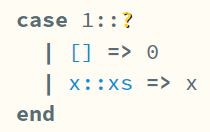
\includegraphics[width=0.25\textwidth]{Media/Figures/unboxing_bug}
\caption{Pattern Matching Bug}
\label{fig:PatternMatchingBug}
\end{figure}

\chapter{Extended Pattern Matching Instantiation}
\label{sec:extendedmatching}
This appendix contains notes on instantiating holes in a match expression according also to the structure of the patterns in a match expression.

To implement this, the scrutinee needs to be matched against a pattern \textit{and} instantiated at the same time. Crucially, instead of just giving up during indeterminate matches, the indeterminate part can be instantiated until it matches.

However, this is not always enough to actually \textit{allow} destructuring using that branch in a match statement. The possibility that \textit{more specific} patterns could be present above the current branch means the resulting instantiation might still be result in an indeterminate match. For example, the following would be an indeterminate match:

\begin{figure}[H]
\texttt{case ?::? | [] => [] | x::y::[] => [] | x::xs => xs}

\caption{More Specific Matches}
\end{figure}

To account for this, we can take ideas from pattern matrix techniques for producing exhaustivity warnings, \cite{PatternMatchingWarnings}. That is, we could generate a set of patterns which explicitly do not match any of the previous branches, then intersect those patterns with the current branch, and instantiate according to this intersection.
\chapter{Supplementary Results and Corpus Data}
\label{sec:results}
The averages for each search method over their successful programs for each implementation are given in \cref{fig:SearchPerformance}. Note that each method succeeds on \textit{differing} sets of programs.

\begin{figure}
  \centering
  \begin{tabular}{lc|cccc}
  & Averages & \multicolumn{4}{c}{\textbf{Implementations}}\\
   & unit & \texttt{DFS} & \texttt{BDFS} & \texttt{IDFS} & \texttt{BFS}\\
   \hline
   \textbf{Time} & ms &  7.6 & 73 & 140 & 120\\
   \textbf{Major Heap} & mB & 3.7 & 32 & 5.9 & 25\\
   \textbf{Minor Heap} & mB & 66 & 680 & 1900 & 1300
  \end{tabular}
  
\caption{Benchmarks: Search Implementations}
\label{fig:SearchPerformance}
\end{figure}


Cast are between slices `from' a type `to' a type. Their average sizes given in \cref{fig:CastSlicingEffectiveness}.

\begin{figure}[h]
  \centering
  \begin{tabular}{lc|cc|cc}
  \multicolumn{2}{c}{\textbf{Averages}} & \multicolumn{4}{c}{\textbf{Subdivisions}}\\
  & & \multicolumn{2}{c|}{\textbf{Ok}} & \multicolumn{2}{c}{\textbf{Errors}}\\ 
   & unit & from & to & from & to\\
   \hline
   \textbf{Cast Slice} & size &  5.5 & 1.2 & 5.9 & 1.5 \\
   Std. dev. &  				 &  8.1 & 3.7 & 7.1 & 2.0\\
   \textbf{Proportion}& \%    & 1 & 0.2 & 1 & 0.2\\
   Std. dev. &  				 &  1 & 0.5 & 1 & 0.4\\
   \multicolumn{6}{c}{\textit{(Unannotated)}}\\
   \textbf{Type Slice} & size &  4.8 & 6.3 & 6.9 & 4.4  \\
   Std. dev. 			&    &  11 & 13 & 9.1 & 9.3\\
   \textbf{Proportion}& \% 	 & 1 & 2 & 2 & 1\\
   Std. dev. &  				 &  1 & 1 & 1 & 1\\
   \multicolumn{6}{c}{\textit{(Annotated)}}
  \end{tabular}
  \caption{Effectiveness: Cast Slices}
\label{fig:CastSlicingEffectiveness}
\end{figure}

Trace length and instantiation size data in \cref{fig:WitnessSize}.
\begin{figure}[h]\centering
\begin{tabular}{l|cccc}
& DFS & BDFS & BFS & IDFS\\
\hline
\textbf{Witness Size} Avg. & 1.1& 1.9&1.4&  2\\
Std. dev. & 1.2& 2.3&1.4&  2.3\\
\textbf{Trace size} Avg. & 33& 32& 11& 17\\
Std. dev. & 35& 33&2.4& 5
\end{tabular}
\caption{Witness \& Trace Sizes}
\label{fig:WitnessSize}
\end{figure}

Some examples of programs in the translated corpus are given in \cref{fig:}. All three were examples where BDFS did not terminate, and are accompanied with their failure classification.

\begin{figure}
\centering
\begin{subfigure}{1\textwidth}
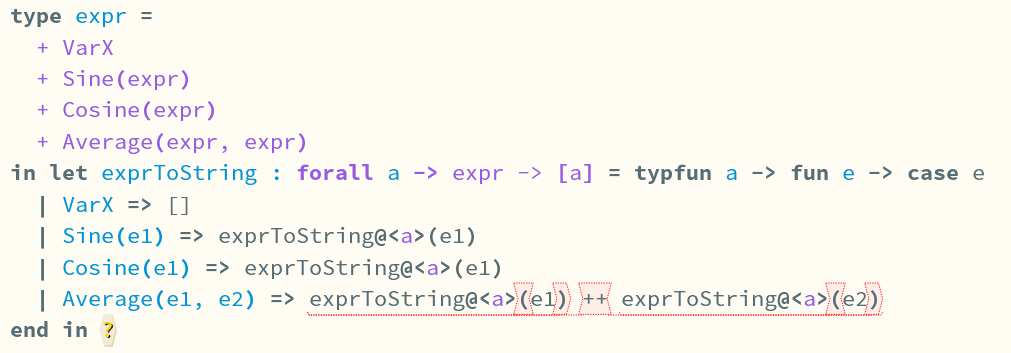
\includegraphics[width=1\textwidth]{Media/Figures/witness_exists}

Depth-first bias caused the procedure to try mostly permutations of \code{Sine(...)} and \code{Cosine(...)}. The error was on the \code{Average(...)} branch, not found within the time limit.
\caption{Witness Exists: prog2270.typed.hazel}
\end{subfigure}

\begin{subfigure}{1\textwidth}
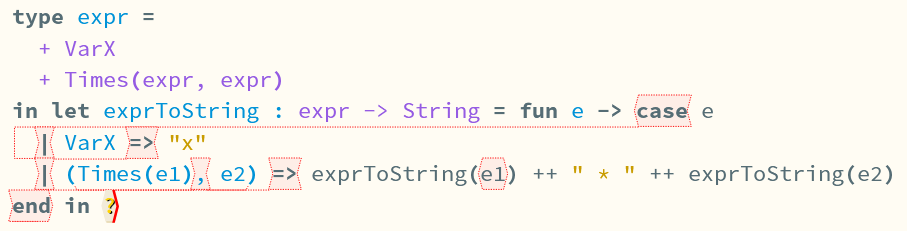
\includegraphics[width=0.8\textwidth]{Media/Figures/dead_code_pattern_instantiation}

A tuple pattern is used when an \code{expr} is expected. Instantiation only tries value of type \code{expr}. Further, another error exists inside this inaccessible branch.
\caption{Dead Code -- Wildcard: prog0080.typed.hazel}
\end{subfigure}

\begin{subfigure}{0.7\textwidth}
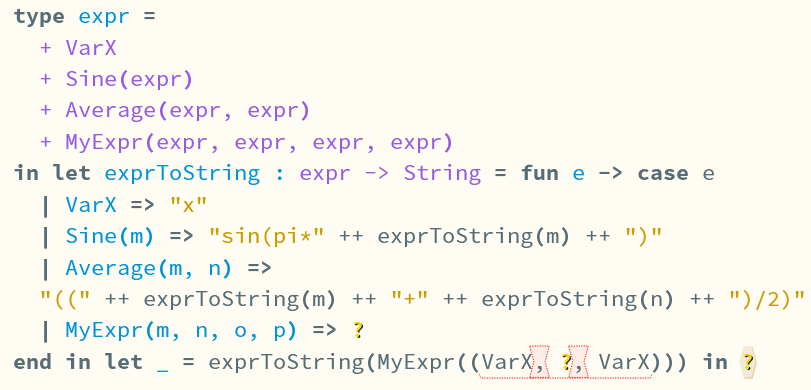
\includegraphics[width=1\textwidth]{Media/Figures/dead_code_wildcard}
Product arity inconsistency is present in inaccessible code bound to the wildcard pattern.
\caption{Dead Code -- Pattern Cast Failure: prog0339.typed.hazel}
\end{subfigure}
\caption{(Paraphrased) Failure Examples}
\label{fig:FailureExamples}
\end{figure}
\chapter{Unimplemented Usability Improvements \& Extensions}\label{sec:UIImprovements}
 Below are proposed improvements, which the architecture of both Hazel and the new features can easily support:

\begin{itemize}
\item Display type slices only \textit{upon request} using the Hazel context inspector, showing the \textit{analysing} and \textit{synthesising} types of the selected expression, see \cref{fig:ContextInspector}.
\item Allow users to deconstruct type slices to query specific parts, e.g. select the just the sub-slice explaining the \textit{return type} of a function or just the function arrow part. This could be done by selecting the type parts in the context inspector.
This interaction would help users really understand how code comes together to define it's types.
\item Visualise graphs of cast dependencies, showing the \textit{execution} context leading to a cast error, summarising more concisely than full evaluation traces.
\item Provide a UI for the search procedure's execution traces and instantiations, integrated with Hazel's trace visualiser. This could include trace compression for better readability (e.g., skipping irrelevant function calls).
\item Implement key bindings to cycle through indeterminate evaluation paths more quickly.
\end{itemize}
\chapter{On Representing Non-Determinism}
\label{sec:NonDeterminismAppendix}

\subsubsection{High Level Representation}
Other high level representations, besides monads, include:

\paragraph{Logic Programming DSL:} Languages like Prolog \cite{Prolog} and Curry \cite{CurryLang} express non-determinism by directly implementing \textit{choice} via non-deterministic evaluation. Prolog searches via backtracking, while Curry abstracts the search procedure.

There are ways to embed this within OCaml. Inspired by Curry, Kiselyov \cite{NondetDSL} created a tagless final style \cite{TaglessFinalDSL} domain specific language within OCaml. This approach fully abstracts the search procedure from the non-deterministic algorithm constructs.
\paragraph{Delimited Continuations:} Delimited continuations \cite{DelimitedControl, ShiftReset} are a control flow construct that captures a portion of the program's execution context (up to a certain delimiter) as a first-class value, which can be resumed later (in OCaml, a function). This enables writing non-deterministic code by duplicating the continuations and running them on each possibility in a choice.

\paragraph{Effect Handlers:} Effect handlers allow the description of effects and factors out the handling of those effects. Non-determinism can be represented by an effect consisting of the choice and fail operators \cite{EffectsExamples, HandlersInAction}, while handlers can flexibly define the search procedure and accounting logic, e.g. storing solutions in a list. As with delimited continuations, to try multiple solutions, the {continuations} must be cloned.


\subsubsection{Reasoning Against}
\paragraph{Direct implementation:} This would not allow for easily abstracting the search order and would obfuscate the workings of the indeterminate evaluation and instantiation algorithms. Some sort of high level representation is also massively beneficial for readability and understanding.
\paragraph{Effect handlers:} Multiple continuation effect handlers were not supported by Javascript of OCaml (JSOO).\footnote{An important dependency of Hazel.} 
\paragraph{Continuations:} Directly writing continuations is difficult and generally more unfamiliar to OCaml developers as opposed to monadic representations.
\paragraph{Optimised DSL}: Introducing a formal DSL including optimisations, such as the proposed Tagless-Final DSL \cite{TaglessFinalDSL, NondetDSL}, is very complex. However, this would allow more flexibility in writing non-deterministic evaluation, with some optimisations made automatically by the DSL.
\chapter{Merges \& Commits}
\label{sec:Merges}
Over the all branches, \textbf{275} commits, excluding merges, were made. Below is a list of merges performed from the Hazel main branch during development and hours taken resolving conflicts with my work. Major merges are in bold, those in red introduced bugs.

\scalebox{0.8}{\begin{tabular}{llcl}
Date & Hash & Time Spent & Description\\
08/04/25 & \tiny{a8efff7cbfdc87eaab3e57d8895562aed1f83a49} & 0m & Formatting fixes\\
08/04/25 &  \tiny{d3da061988cb0d4174a36282d9588d20d11d8ebd} & 15m & Updated Dependencies\\
08/04/25 & \tiny{33d80b9ae3fa7ade69bbefee1dcc10aaaebc11d1} & 20m & {\color{red}Probes} \& Live Projectors\\
\textbf{08/04/25} & \tiny{96adcc111a650ed2d709a965adcac14e7197ccc5} & \textbf{45m }& \textbf{Syntax Factory}\\
\textbf{08/04/25} & \tiny{2d1ab30445ecce5ce3d0f79b2b714031fd762af0} & \textbf{50m} & \textbf{Id tagging a type parameter}\\
\textbf{08/04/25} & \tiny{451e6f76b56874ec3ffa02002cf6a4013193d9d9}& \textbf{2h 15m} & \textbf{\color{red}Pattern coverage rework}\\
08/04/25& \tiny{117f689dda9794515b5c464d246a792e67416551} & 0m & Context inspector fixes\\
08/04/25& \tiny{672f7ed7814a42b93f3e4efa4a390534c25d35ad} & 0m & Double parenthesisation fixes\\
08/04/25& \tiny{971763990ead191077249c72740b3ad6a657dfda} & 0m & Code coverage settings\\
08/04/25& \tiny{7404b6cfdc3c4b683aa6723532eb62ca7085e33f} & 0m & Bring back function names\\
08/04/25& \tiny{5f18db680913ce8be1d795d20bd54bf2f5e89f01} & 10m & Unboxing fixes\\
08/04/25& \tiny{f197b65e0fb00fbc7c86a15005cd6a7ed376ac46} & 0m & Code coverage support\\
08/04/25& \tiny{fbf415ea3347971672e50665ae4616d98409f087} & 0m & Cast \& TypFun bugfix\\
08/04/25& \tiny{661eae7621e509d762715eeecd56888078faf9b8} & 10m & {\color{red}Make join symmetric}\\
08/04/25& \tiny{f288788ae026a18bc3cd361da6e12ee716cc8723} & 0m & Editor statics fixes\\
08/04/25& \tiny{b671df993ea19171c21cd248e6857ad932baf9f3} & 0m & Structure editor polishing\\
07/04/25& \tiny{d7a2e2a242a474c0e50abec8659004a7ee2ab034} & \textbf{7h} & \textbf{\color{red}Labelled Tuples}\\
06/04/25 & \tiny{18185d16f23d79be47e7282aae7d0b1f77c4ed88} & 10m & Evaluator clean-up\\
06/02/25 & \tiny{f082201f1cf606068bb037a0da1c896f585e4974} & 30m & Fix generalised closures\\
31/01/25 & \tiny{c6f23de39b5e64e352e4d7cbab5082cc50f3b658} & 10m & Add builtins \& bugfixes\\
17/12/24 & \tiny{0dd744b1c28ca1c11dfb6368051633dcc56b8353} & 0m & Add tests\\
16/12/24 & \tiny{a145ac508b5a50b132f463b2ad670d6eaa3d3b84} & 0m & Stepper UI fixes\\
\textbf{11/12/24} & \tiny{8b189bd667ac0f1a91a18781bb5db183c58ba29f} & \textbf{5h} &\textbf{ MVU UI overhaul}\\
\end{tabular}}

\backmatter
\chapter{Project Proposal}
\label{sec:ProjectProposal}
\section{Description}
This project will add some features to the Hazel language \cite{Hazel}. Hazel is a functional research language that makes use of gradual types to support unusual features such as: holes (code placeholders) to give type meaning to incomplete programs. Importantly for this project, all Hazel programs, even ill-typed or incomplete programs, are evaluable. This allows dynamic reasoning about ill-typed programs via evaluation traces with the potential to improve the user's understanding of \textit{why ill-typed programs go wrong}. See example below:\par
\begin{minted}[escapeinside=||]{reason}
let rec sum : Int -> Int = fun n ->
  if n == 0 then
    |\error{\texttt{true}}|    // Type error statically caught and correctly localised
  else
    n + sum(n - 1)
in sum(2)
\end{minted}
But evaluation is still possible; see below a (compressed) trace to a stuck value exhibiting a cast error:
\[\code{sum(2)} \mapsto^{*} \code{2 + sum(1)} \mapsto^{*} \code{2 + (1 + } \casterror{Bool}{Int}{ true}\code{)}\]
 
This project aims to exploit further this potential by providing some extra features to both: aid with finding values/inputs that demonstrate why type-errors were found (type-error witnesses) and linking the evaluation traces back to source code. But is not expected to directly measure the usefulness of such evaluation traces themselves in debugging, nor is the design space for a Hazel debugger inspecting and interacting with traces to be explored.\par 
Searching for type-error witnesses automatically is the main feature provided by this project, inspired by Seidel et al.\  \cite{SearchProc}. The intended use of this is to automatically generate values (for example, function arguments) that cause ill-typed programs to `go wrong' (lead to a cast error). More specifically, the search procedure can be thought of as evaluating a \textit{special hole} which refines its type dynamically and non-deterministically instantiates itself to values of this type to find a value whose evaluation leads to a \textit{general} cast error -- `general' meaning excluding trivial cast errors such as generating a value that doesn't actually have the refined expected type.  \par 
Such a search procedure is undecidable and subject to path explosion, hence the success criteria (detailed below) does not expect witnesses to be provided in general, even if they do exist. Sophisticated heuristics and methods to limit path explosion to support large code samples is not a core goal.\par 

Formal semantics of this procedure and associated proofs is an extension goal, consisting of preservation proofs and witness generality proofs (formalising the notion of generality mentioned previously).\par

Secondly, \textit{cast slicing} will track source code that contributed to any cast throughout the cast elaboration and evaluation phases.  In particular, this allows a cast involved in a cast error relating to a type-error witness to point back to offending code. This is expected in some sense to be similar to blame tracking \cite{Blame}, error and dynamic program slicing \cite{ErrSlice, DynProgSlice}, although these are not directly relevant for this project.\par 

Work required for the creation of an evaluation corpus of ill-typed hazel programs, requiring manual work or creation of automated translation and/or fuzzing tools, is timetabled.

\section{Starting Point}
Only background research and exploration has been conducted. This consists of reading the Hazel research papers \cite{Hazel} and various other related research topics including: gradual types, bidirectional types, symbolic evaluation, OCaml error localisation and visualisation techniques.\par 
More research, into the Hazel codebase in particular, and concrete planning is required and is timetabled accordingly.

\section{Success Criteria}
Core goals are the minimum expected goals that must be completed to consider this project a success. This corresponds to a working tool for a large portion of Hazel.\par 
Extension goals will be timetabled in, but are relatively more difficult and not required for the project to be considered a success.\par 

First, I give some definitions of terms:
\begin{itemize}
\item \textbf{Core Calculus} -- The formal semantics core of Hazel as referred to by the Hazel research papers \cite{HazelLivePaper}.
\item \textbf{Basic Hazel} -- A Hazel subset consisting of the core calculus, product and sum types, type aliases, bindings, (parametric) lists, bools, int, floats, strings, and their corresponding standard operations.
\item \textbf{Full Hazel} -- Hazel, including \textbf{Basic Hazel} plus pattern matching, explicit impredicative system-F style polymorphism and explicitly recursive types.
\item \textbf{Core Corpus} -- A corpus of ill-typed Hazel programs that are similar in complexity and size to student programs being taught a functional language, \textit{e.g. (incorrect) solutions to the ticks in FoCS}. This will include examples in \textbf{Basic} or \textbf{Full Hazel} as required.
\item \textbf{Extended Corpus} -- A corpus of ill-typed Hazel programs that are larger in size, more akin to real-world code.
\item \textbf{Evaluation Criteria} -- Conditions for the search procedure to meet upon evaluation:
\begin{enumerate}
\item Must have reasonable coverage --  success in finding an \textit{existing} witness which is correct and general.
\item Must find witnesses in an amount of time suitable for interactive debugging -- in-line with build-times for a debug build of existing languages.
\end{enumerate}
\end{itemize}
\subsection{Core Goals}
\begin{itemize}
\item Success criteria for Cast Slicing -- Cast slicing must be \textit{correct} (slices must include all code involved in the cast) and work for \textit{all casts}, including casts involved in cast errors. Informal reasoning in evidence of satisfying these conditions is all that will be required. 
\item Success criteria for the Search Procedure -- The procedure must work for \textbf{Basic Hazel}, meeting the \textbf{Evaluation Criteria} over the \textbf{Core Corpus}. Analysis of some classes of programs for which witnesses could not be generated is also expected.
\end{itemize}
\subsection{Extension Goals}
\begin{itemize}
\item Search Procedure Extensions -- Support for \textbf{Full Hazel} under the same criteria as above.
\item Search Procedure Performance Extensions -- Meeting of the \textbf{Evaluation Criteria} over an \textbf{Extended Corpus}
\item Formal Semantics -- The specification of a formal evaluation semantics for the search procedure over the \textbf{Core Calculus}. Additionally, a preservation and witness generality proof should be provided.
\end{itemize}

\section{Work Plan}
\subsection*{21st Oct \textit{(Proposal Deadline)} -- 3rd Nov}
Background research \& research into the Hazel semantics, cast elaboration, type system, and codebase. Produce implementation plan for cast slicing and the search procedure for the \textbf{Core Calculus}. This includes an interaction design plan, expected to be very minimal.\par
\textit{Milestone 1: Plan Confirmed with Supervisors}

\subsection*{4th Nov -- 17th Nov}
Complete implementation of Cast Slicing for the \textbf{Core Calculus}. Write detailed reasoning for correctness, including plan for \textbf{Basic Hazel}. Add unit testing.\par 
\textit{Milestone 2: Cast slicing is complete for the \textbf{Core Calculus}.}

\subsection*{18th Nov -- 1st Dec \textit{(End of Full Michaelmas Term)}}
Complete implementation of the search procedure for the \textbf{Core Calculus}. \par 
\textit{Milestone 3: Search Procedure is complete for the \textbf{Core Calculus}.}

\subsection*{2nd Dec -- 20th Dec}
Extension of both cast slicing and the search procedure to \textbf{Basic Hazel}.\par 
\textit{Milestone 4: Cast slicing \& search procedure are complete for \textbf{Basic Hazel}}

\subsection*{21st Dec -- 24th Jan \textit{(Full Lent Term starting 16th Jan)}}
Basic UI interaction for the project. Drafts of Implementation chapter. Slack time. Expecting holiday, exam revision, and module exam revision. Should time be available, the \textbf{Formal Semantics} extension will be attempted.\par
\textit{Milestone 5: Implementation chapter draft complete.}

\subsection*{25th Jan -- 7th Feb \textit{(Progress Report Deadline)}}
Writing of Progress Report. Planning of evaluation, primarily including decisions and design of tools to be used to collect/create the \textbf{Core Corpus} and planning the specific statistical tests to conduct on the corpus. Collected corpus and translation method will be one of:
\begin{enumerate}
\item Manual translation of a small ill-typed OCaml program corpus into ill-typed Hazel.
\item Manual insertion of type-errors into a well-typed Hazel corpus.
\item Collection of a well-typed Hazel corpus.\\ 
Tools: A Hazel type fuzzer to make the corpus ill-typed.
\item Collection of a well-typed OCaml corpus.
\\Tools: OCaml -> Hazel translator/annotator which works with well-typed OCaml. A Hazel type fuzzer.
\item Collection of an ill-typed OCaml corpus. 
\\Tools: OCaml -> Hazel translator which works with ill-typed OCaml. \textit{This would NOT be expected to be an implicitly typed Hazel front-end which maintains desireable properties like parametricity.} 
\end{enumerate}
\textit{Milestone 6: Evaluation plan and corpus creation method confirmed with supervisors.}\\
\textit{Milestone 7: Underlying corpus (critical resource) collected.}

\subsection*{8th Feb -- 28th Feb}
Implementation of the required tools for evaluation as planned. Some existing code or tools may be re-used, such as the OCaml type-checker.\par
\textit{Milestone 8: \textbf{Core Corpus} has been collected.}

\subsection*{1st Mar -- 15th Mar \textit{(End of Full Lent Term)}}
Conducting of evaluation tests and write-up of evaluation draft including results.\par
\textit{Milestone 9: Evaluation results documented.}\\
\textit{Milestone 10: Evaluation draft complete.}

\subsection*{16th Mar -- 30th Mar}
Drafts of remaining dissertation chapters. If possible, collection and evaluation of \textbf{Extended Corpus} using the same tools as the \textbf{Core Corpus}.\par

\textit{Milestone 11: Full dissertation draft complete and sent to supervisors for feedback.}

\subsection*{31st Mar -- 13th Apr}
Act upon dissertation feedback. Exam revision.\par
\textit{Milestone 12: Second dissertation draft complete and send to supervisors for feedback.}

\subsection*{14th Apr -- 23rd Apr \textit{(Start of Full Easter Term)}}
Act upon feedback. Final dissertation complete. Exam revision.\par

\textit{Milestone 13: Dissertation submitted.}

\subsection*{24th Apr -- 16th May \textit{(Final Deadline)}}
Exam revision.\par
\textit{Milestone 14: Source code submitted.}

\section{Resource Declaration}
\begin{itemize}
\item Underlying Corpus of either: Well-typed OCaml programs, Ill-typed OCaml programs, Hazel programs. For use in evaluation. The required tools or manual translation to convert these into the ill-typed Hazel \textbf{Core Corpus} are detailed and allocated time in the timetable.

\item Hazel source code. Openly available with MIT licence on GitHub \cite{HazelCode}.

\item My personal laptop will be used for development, using GitHub for version control and backup of both code and dissertation. I accept full responsibility for this machine and I have made contingency plans to protect myself against hardware and/or software failure. A backup pc is available in case of such failure.

\end{itemize}
%TC:endignore

\end{document}